\PassOptionsToPackage{full}{textcomp}
% include symmetric to place margins left and right instead of right only
% nohyper, nobib?
\documentclass[nobib,a4paper,twoside,notoc,justified,marginals=justified]{tufte-book}
% \documentclass{caesar_book}
\usepackage[utf8]{inputenc}

% \usepackage{hyperref}
\hypersetup{colorlinks}

% \usepackage{setspace}
% \newcommand{\newthought}[1]{\textsc{#1}}

%%
% For nicely typeset tabular material
\usepackage{booktabs, tabularx, tabulary}

% fix too many alphabets error
\usepackage{amsmath, amssymb}
\newcommand\hmmax{0}
\newcommand\bmmax{0}

\AtBeginDocument{\setlength{\parindent}{0em}}

% fix margins?
% \usepackage{marginfix}

\usepackage{enumitem, bm, xcolor, braket, dsfont, graphicx, cancel}
\usepackage[multidot]{grffile}
% \usepackage[colorlinks, linkcolor = red, citecolor = black, filecolor = black, urlcolor = blue]{hyperref} 
% \usepackage{nameref}
% \hypersetup{colorlinks}
\usepackage{algorithmic}
\usepackage{todonotes}

% Quotes
\usepackage{epigraph}
\setlength\epigraphwidth{10cm}
\setlength\epigraphrule{0pt}

%% style
% \usepackage{mathptmx}
% \usepackage{setspace}
% \linespread{1.0}

% \iflarger
%\AtBeginDocument{%
%	\fontsize{12}{14}\selectfont
%}%
% \else\fi


% integrate amsthm and txmath
\usepackage{savesym}
\usepackage{amsthm}
\savesymbol{openbox}
\usepackage{newtxtext,newtxmath}
\restoresymbol{TX}{openbox}

% theorems
\newtheorem*{theorem}{Theorem}
\newtheorem*{thm}{Theorem}

% shorthand
\renewcommand{\t}[1]{\text{#1}}
\renewcommand{\d}{{\rm d}}
\renewcommand{\b}[1]{{\bf #1}}
\newcommand{\B}[1]{\mathbf{#1}}
\newcommand{\D}[1]{{#1}^\dagger}
\newcommand{\fD}[1]{{#1}^{ \phantom{\dagger}}}
\renewcommand{\P}[1]{{#1}^\prime}
\newcommand{\fP}[1]{{#1}^{\phantom{\prime}}}
\newcommand{\im}{{\rm i}}
\newcommand{\halb}{\frac{1}{2}}
\DeclareMathOperator{\Tr}{Tr}
\newcommand{\kb}{k_{\rm B}}
\newcommand{\sigmaA}{\sigma^\mathrm{A}}
\newcommand{\sigmaAOS}{\sigma^\mathrm{A}_\mathrm{OS}}
\newcommand{\sigmaAMD}{\sigma^\mathrm{A}_\mathrm{MD}}
\newcommand{\tcut}{t_{\rm c}}
\newcommand{\teff}{t^{\rm eff}_0}

% transpose
\usepackage{relsize}
\newcommand{\tp}[1]{{#1}^{\mathrm t}}
% \!\: = 1mu distance; \!\; = 2mu (\, = 3mu)
\newcommand{\itp}[1]{{#1}^{\!\:\scalebox{0.55}[1.0]{\( - \)}1 \mathrm t}}

% comments:
% dblue: https://coolors.co/1f77b4
\definecolor{dblue}{RGB}{31,119,180}
\definecolor{dblue_light}{HTML}{5AAAE3}
\definecolor{purple_light}{HTML}{A61EB3}
\definecolor{yellow1}{HTML}{E7EB90}
\definecolor{yellow2}{HTML}{FADF63}
\definecolor{yellow3}{HTML}{E6AF2E}
\definecolor{red_light}{HTML}{FE404A}
\definecolor{cite}{HTML}{2BB31E}
\definecolor{djordje}{RGB}{192,225,215}
\definecolor{matthias1}{HTML}{EE9484}
\definecolor{matthias2}{HTML}{DC3A1E}

\newcommand{\MOVE} [1] 
{\todo[inline,backgroundcolor=red_light, bordercolor=white]{{\bf MOVE:} #1}}
\newcommand{\REM} [1] 
{\todo[inline,backgroundcolor=dblue_light, bordercolor=white]{{\bf REM:} #1}}
\newcommand{\CITE} [1] 
{\todo[inline,backgroundcolor=cite, bordercolor=white]{{\bf CITE:} #1}}
% \newcommand{\FK}[1]{\textcolor{blue}{{\bf #1 }}}
\newcommand{\TODO} [1] 
{\todo[inline,backgroundcolor=red, bordercolor=white]{{\bf TODO:} #1}}
\newcommand{\ADD} [1] 
{\todo[inline,backgroundcolor=red, bordercolor=white]{{\bf ADD} #1}}
\newcommand{\FK} [1] 
{\todo[inline,backgroundcolor=yellow2, bordercolor=white]{{\bf Florian:} #1}}
\newcommand{\idea} [1] 
{\todo[inline,backgroundcolor=red, bordercolor=white]{{\bf idea:} #1}}
\newcommand{\inlinecomment}[1]{\textcolor{red}{{\bf #1 }}}
\newcommand{\prelim}[1]{\textcolor{red}{{\bf prelim:} {\it #1 }}}
\newcommand{\CC} [1] 
{\todo[inline,backgroundcolor=yellow3, bordercolor=white]{{\bf CC:} #1}}
\newcommand{\CHECK}{\todo{check}}
\newcommand{\mscomment} [1] 
{\todo[inline,backgroundcolor=matthias1, bordercolor=white]{{\bf Matthias comment:} #1}}
\newcommand{\mscorrect} [1] 
{\todo[inline,backgroundcolor=matthias2, bordercolor=white]{{\bf Matthias correction:} #1}}
% Tufte

% TOC
% https://tex.stackexchange.com/questions/121790/how-to-generate-a-full-width-table-of-contents-tufte-book
\usepackage{lipsum,mdframed}
\definecolor{secnum}{RGB}{13,151,225}
\definecolor{ptcbackground}{RGB}{212,237,252}
\definecolor{ptctitle}{RGB}{0,177,235}

\setcounter{secnumdepth}{3}

\usepackage[toc]{appendix}
% \usepackage{titletoc}
% \usepackage{etoolbox}
\setcounter{tocdepth}{1}
%\pretocmd{\tableofcontents}{\begin{mdframed}\let\cleardoublepage\relax}{}{}
%  \apptocmd{\tableofcontents}{\end{mdframed}}{}{}

% The fancyvrb package lets us customize the formatting of verbatim
% environments.  We use a slightly smaller font.
\usepackage{fancyvrb}
\fvset{fontsize=\normalsize}

%%
% Prints argument within hanging parentheses (i.e., parentheses that take
% up no horizontal space).  Useful in tabular environments.
\newcommand{\hangp}[1]{\makebox[0pt][r]{(}#1\makebox[0pt][l]{)}}

%%
% Prints an asterisk that takes up no horizontal space.
% Useful in tabular environments.
\newcommand{\hangstar}{\makebox[0pt][l]{*}}

%%
% Prints a trailing space in a smart way.
\usepackage{xspace}

% Prints the month name (e.g., January) and the year (e.g., 2008)
\newcommand{\monthyear}{%
  \ifcase\month\or January\or February\or March\or April\or May\or June\or
  July\or August\or September\or October\or November\or
  December\fi\space\number\year
}

% http://tex.stackexchange.com/a/140164/1913
% \ifxetex
% xetex fix https://tex.stackexchange.com/a/200725/91226
%\ifx\ifxetex\ifluatex\else % if lua- or xelatex   \newcommand{\textls}[2][5]{%
%    \begingroup\addfontfeatures{LetterSpace=#1}#2\endgroup
%  }
%  \renewcommand{\allcapsspacing}[1]{\textls[15]{#1}}
%  \renewcommand{\smallcapsspacing}[1]{\textls[10]{#1}}
%  \renewcommand{\allcaps}[1]{\textls[15]{\MakeTextUppercase{#1}}}
%  \renewcommand{\smallcaps}[1]{\smallcapsspacing{\scshape\MakeTextLowercase{#1}}}
%  \renewcommand{\textsc}[1]{\smallcapsspacing{\textsmallcaps{#1}}}
%\fi


% Prints an epigraph and speaker in sans serif, all-caps type.
\newcommand{\openepigraph}[2]{%
  %\sffamily\fontsize{14}{16}\selectfont
  \begin{fullwidth}
  \sffamily\large
  \begin{doublespace}
  \noindent\allcaps{#1}\\% epigraph
  \noindent\allcaps{#2}% author
  \end{doublespace}
  \end{fullwidth}
}

% Inserts a blank page
\newcommand{\blankpage}{\newpage\hbox{}\thispagestyle{empty}\newpage}

\usepackage{units}

% Typesets the font size, leading, and measure in the form of 10/12x26 pc.
\newcommand{\measure}[3]{#1/#2$\times$\unit[#3]{pc}}

% Macros for typesetting the documentation
\newcommand{\hlred}[1]{\textcolor{Maroon}{#1}}% prints in red
\newcommand{\hangleft}[1]{\makebox[0pt][r]{#1}}
\newcommand{\hairsp}{\hspace{1pt}}% hair space
\newcommand{\hquad}{\hskip0.5em\relax}% half quad space
\newcommand{\na}{\quad--}% used in tables for N/A cells

% Generates the index
\usepackage{makeidx}
\makeindex


\begin{document}

% Front matter
\frontmatter
\addtocontents{toc}{\protect\setcounter{tocdepth}{0}}
  
%  % r.1 blank page
%  \blankpage
%  
%% r.3 full title page
%\maketitle

% r.5 contents
\tableofcontents

% \listoffigures

% \listoftables

% r.7 dedication
%\cleardoublepage
%~\vfill
%\begin{doublespace}
%  \noindent\fontsize{12}{12}\selectfont\itshape
%  \nohyphenation
%  \hfill To my teachers.
%\end{doublespace}
%\vfill
%\vfill


% r.9 introduction
\cleardoublepage

% \chapter{Introduction}
% \epigraph{\singlespacing \it ``Die Zeit des unbedenklichen Wirtschaftens mit den Energiequellen und Stofflagern, die uns die Natur zur Verfügung gestellt hat, wird wahrscheinlich schon für unsere Kinder nur noch die Bedeutung einer vergangenen Wirtschaftsepoche haben.''}{W. Schottky, 1929~\cite{Schottky1929}}
% [ ] Why thermal conductivity?
% [ ] Why novel thermal insulators?
% [ ] Why computational materials science?
\newthought{One of the major challenges} humankind faces in the 21th century is the responsible and sustainable handling of the earth's natural resources.  Yet, most energy today is lost as waste heat during the transformation of raw energy sources to usable power. To date, there is no fuel based heat engine that exceeds an efficiency of 50\,\% and often it is even worse~\cite{eia}. 
Since gas- and aircraft-turbines are essentially Carnot engines, their efficiency and core power are directly related to the combustion temperature~\cite{Clarke2012,Perepezko2009}. This has been utilized during the past 30 years by developing 
ceramics with high thermal resistivity that are nowadays applied as \emph{thermal barrier coatings} on turbine airfoils in heat engines~\cite{Clarke2003}. A thermal barrier coating serves as a thin, extremely heat insulating layer and thus allows to operate a turbine at higher temperatures, thereby increasing its efficiency.

A complementary strategy is to recycle waste heat where it occurs. One way to do so is to use the
\emph{thermoelectric effect} to  generate electric power from temperature gradients~\cite{Snyder2008}. The main obstacle preventing mass operation though is the limited conversion rate (figure of merit) $zT$ of even the most advanced thermoelectric materials known to date. To make matters worse, these materials often contain heavy metals and are toxic, and their manufacturing process is difficult and expensive~\cite{Nolas2001}. Recent advancements in the field, such as the discovery of a high thermoelectric figure of merit in the lead-free material Tin Selenide~\cite{Zhao2014}, offer hope that novel materials with significant figure of merit can be found that are non-toxic, easy and cheap to produce, and consist of abundant elements.

\newthought{A key physical property} of both thermal barrier coatings (TBCs) and thermoelectrics is their thermal conductivity $\kappa$. In the case of thermoelectrics, the figure of merit is inversely proportional to $\kappa$~\cite{Nolas2001}:
\begin{align}
zT = \frac{S^2 \sigma_{\rm el}}{\kappa} T~,
\label{eq:zT}
\end{align} 
where $T$ dentoes the temperature, $S$ the Seebeck coefficient, and $\sigma_{\rm el}$ is the electrical conductivity.
A prerequisite to finding better thermoelectrics or TBCs therefore is to find materials which are thermally insulating. These are typically non-metals, since the free electrons in metals are good heat carriers, and most of the known thermoelectrics are thermally insulating inorganic semiconductors~\cite[p.\,15]{Nolas2001}.

% [ ] say sth. about microstructuring?

Despite the technological needs, systematic knowledge of thermal conductivities in inorganic compounds is scarce. A renowned database like Springer Materials only lists thermal conductivities for about 200~of these compounds~\cite{SpringerMaterials}, which is partially due to the fact that accurate measurements of thermal conductivity are tricky to perform[\REM{citation!}]. As a consequence, thermal conductivity is not systematically understood beyond semi-empirical and phenomenological trends in a very limited number of simple material classes~\cite{morelli2006}.

\newthought{The aim of this work} is to open a new pathway for overcoming the problem of limited data by devising a route to systematically scan material space for thermal insulators and calculate their thermal conductivities from first principles. This route is twofold: After reviewing the relevant theoretical tools necessary to simulate heat transport in thermal insulators, we describe how to assess a key physical property shared by most thermal insulators,~.i.\,e.,~\emph{anharmonicity}, without the need for explicit model building beyond the harmonic approximation.

\section*{Organization of the Thesis}
\TODO{Derive all the formulas, discuss anharmonicity, present thermal conductivity}

%%
% Start the main matter (normal chapters)
\mainmatter
\addtocontents{toc}{\protect\setcounter{tocdepth}{1}}  % later -> 1

% \part{Theoretical Foundation}

\chapter{The Many Body Problem}
\epigraph{\singlespacing \it ``The underlying physical laws necessary
for the mathematical theory of a large part of physics and the whole of chemistry
are [...] completely known, and the difficulty is only that the exact application
of these laws leads to equations much too complicated to be soluble. It therefore becomes desirable that approximate practical methods of applying quantum
mechanics should be developed, which can lead to an explanation of the main
features of complex atomic systems without too much computation.''}{P.A.M. Dirac, 1929~\cite{Dirac.1929}}

\newthought{In this chapter}, we summarize the theoretical background of {\it ab initio} simulations starting from the non-relativistic, time-independent Schrödinger equation for a general many-body system.

\section{The Many Body Hamiltonian}

The full (non-relativistic) many body Hamiltonian in the absence of external electromagnetic fields for an otherwise arbitrary system reads
\begin{align}
    \hat{H}
        = \hat{{T}}^{\mathrm{e}}
        + \hat{{V}}^{\mathrm{e}-\mathrm{e}}
        + \hat{{V}}^{\mathrm{e}-\mathrm{Nuc}}
        + \hat{{V}}^{\mathrm{Nuc}-\mathrm{Nuc}}
        + \hat{{T}}^{\mathrm{Nuc}}~,
    \label{eq:Hamiltonian}
\end{align}
where
\begin{align}
    \hat T^{\rm e} 
        =\sum_{i} \frac{\hat{\mathbf{p}}_{i}^{2}}{2 m_{\rm e}}
    \label{eq:Te}
\end{align}
is the kinetic energy operator for electrons of mass $m_{\rm e}$ with momentum operators $\hat{\bf p}_i$, and 
\begin{align}
    \hat V^{\rm e-e}
        = \sum_{i < j} \frac{e^{2}}{\left|\hat{\b r}_{i}-\hat{\bf r}_{j}\right|}~,
    \label{eq:Ve}
\end{align}
is the Coulombic electron-electron repulsion operator with the electronic position operators $\hat{\bf r}_i$ and the elementary charge $e$. 
The Coulomb attraction between the negatively charged electrons and the positively charged nuclei reads
\begin{align}
    \hat V^{\rm e-Nuc}
        = -\sum_{i, J} \frac{Z_J e^{2}}{\left|\hat{\b r}_{i}-\hat{\bf R}_{J}\right|}~,
    \label{eq:Venuc}
\end{align}
where $Z_J$ denotes the charge number of nucleus $J$, and $\hat{\bf R}_J$ is the nuclear position operator. 
Accordingly, we define the nuclear-nuclear repulsion as
\begin{align}
    \hat V^{\rm Nuc-Nuc}
        = \sum_{I < J} \frac{Z_{I} Z_{J} e^{2}}{\left|\hat{\b R}_{I}-\hat{\bf R}_{J}\right|}~,
    \label{eq:Vnuc}
\end{align}
and the kinetic energy operator for nuclei with momentum operators $\hat{\bf P}_I$ and masses $M_I$ reads
\begin{align}
    \hat T^{\rm Nuc} 
        =\sum_{I} \frac{\hat{\mathbf{P}}_{I}^{2}}{2 M_{I}}~.
    \label{eq:Tnuc}
\end{align}
This Hamiltonian governs the dynamical evolution of a many-particle system represented by a state $\ket{\Psi}$ via the time dependent Schr\"odinger equation,
\begin{align}
	\hat H \ket{\Psi} = \im \hbar \frac{\partial}{\partial t} \ket{\Psi}~,
	\label{eq:TdSE}
\end{align}
from which all material properties (neglecting relativistic and effects and electromagnetic fields) follow.

\section{The Born-Oppenheimer Approximation}
We go over to a unitless Hamiltonian by scaling Eq.\,\eqref{eq:Hamiltonian} with the Hartree energy $E_{\rm h} = m_{\rm e} e^4 / \hbar^2 \approx 27.2\,{\rm eV}$, where $\hbar$ denotes the Planck constant. Distances are expressed in terms of the Bohr radius $a_0 = \hbar^2 / m e^2$ such that~$\hat{\bf r} \equiv {\bf r} = a_0 \tilde{\bf r}$, and the momentum operators are replaced by the respective differential operators, $\hat{\bf p}=-\im \hbar \partial / \partial {\bf r}$~\cite{Czycholl}. We find
\begin{align}
\begin{split}
    \tilde H 
        \equiv& ~\hat{H} / E_{\rm h} \\
        =& 
        - \frac{1}{2} \sum_i \frac{\partial^2}{\partial \tilde{\bf r}_i^2}
        + \sum_{i < j} \frac{1}{\left|\tilde{\b r}_{i}-\tilde{\bf r}_{j}\right|}
        - \sum_{i, J} -\frac{Z_J}{\left|\tilde{\b r}_{i}-\tilde{\bf R}_{J}\right|}
        + \sum_{I < J} \frac{Z_{I} Z_{J}}{
            \left|\tilde{\b R}_{I}-\tilde{\bf R}_{J}\right|} 
        \\
        &- \underset{\tilde{T}^{\rm Nuc}}{\underbrace{\frac{1}{2} \sum_I \frac{m_{\rm e}}{M_I} \frac{\partial^2}{\partial \tilde{\bf R}_I^2}}}~,
    \label{eq:Hscaled}
\end{split}
\end{align}
which depends on the charge numbers $\{Z_I\}$ and the mass ratios $\{ m_{\rm e} / M_I \}$. From this viewpoint, we see that the relative order of magnitude of the nuclear kinetic energy $\hat{T}^{\rm Nuc}$ is \mbox{$m_{\rm e} / M_I \approx 10^{-4} - 10^{-5}$}. 
We therefore expand the total energy in powers of the mass ratio $m/M$ using the electronic contributions as reference,
%This means that the nuclear kinetic energy can be treated as a perturbation term with respect to the electronic and electron-nuclear contributions,
%\mscomment{this is not perturbation theory (so far)}
%\FK{rephrase: ... total energy can be expanded in powers of the mass ratio $m/M$ using the el/el-nuc contributions as reference}
\begin{align}
    \hat{H}   &= \hat{H}^0 + \hat{T}^{\rm Nuc} + {\hat{V}}^{\mathrm{Nuc}-\mathrm{Nuc}}~, \text{ where} 
    \label{eq:H=H0+T}
    \\
    \hat{H}^0 &=
          {\hat{T}}^{\mathrm{e}}
        + {\hat{V}}^{\mathrm{e}-\mathrm{e}}
        + {\hat{V}}^{\mathrm{e}-\mathrm{Nuc}}~.
    \label{eq:H0}
\end{align}
%
%\mscomment{move nuc-nuc to 1.9 bc it is computed w.r.t. to el. wavefunctions}
%\FK{check}
In this notation, the time-independent many-body Schr\"odinger equation reads
\begin{align}
    \hat{H} \psi ({\bf r}, {\bf R}) = E \psi ({\bf r}, {\bf R})~,
    \label{eq:Schroedinger1}
\end{align}
with ground-state eigenvalues $E$ and many-body wave functions \mbox{$\psi ({\bf r}, {\bf R})$}, where {${\bf r} = ({\bf r} \ldots {\bf r}_{N_{\rm e}})$} denotes all electronic coordinates, and ${\bf R} = ({\bf R}_1 \ldots {\bf R}_{N_{\rm Nuc}})$ the nuclear coordinates, respectively. According to Eq.\,\eqref{eq:H=H0+T}, we expand the wave functions $\psi ({\bf r}, {\bf R})$ in a complete set of orthonormal basis functions $\phi_l$,
\begin{align}
\psi ({\bf r}, {\bf R}) = \sum_l \chi_l ({\bf R}) \phi_l ({\bf r}; {\bf R})~,
\label{eq:psi_expansion_phi}
\end{align}
where the $\phi_l$ are the solutions to the Hamiltonian $\hat{H}^0$,
\begin{align}
    \hat{H}^0 \phi_l ({\bf r}; {\bf R})
        = E^0_l ({\bf R}) \phi_l ({\bf r}; {\bf R})~.
    \label{eq:Hsolution1}
\end{align}
The functions $\phi_l$ and the eigenvalue $E_l^0({\bf R})$ depend \emph{parametrically} on $\bf R$, which means that they are obtained for a nuclear configuration $\bf R$ regarded as fixed.
The nuclear functions $\chi_l$ are determined by using the expanded wavefunction $\psi$ given by Eq.\,\eqref{eq:psi_expansion_phi} in the full Schr\"odinger equation~\eqref{eq:Schroedinger1},
\begin{align}
    (\hat{H} - E) \psi ({\bf r}, {\bf R})
        & = \sum_l (\hat{T}^{\rm Nuc} + {{V}}^{\mathrm{Nuc}-\mathrm{Nuc}} ({\bf R}) + \hat{H}^0 - E) \chi_l ({\bf R}) \phi_l ({\bf r}, {\bf R}) \nonumber \\
        &= \sum_l (\hat{T}^{\rm Nuc} + {{V}}^{\mathrm{Nuc}-\mathrm{Nuc}} ({\bf R}) + E^0_l({\bf R}) - E) \chi_l ({\bf R}) \phi_l ({\bf r}, {\bf R}) = 0~,
\end{align}
%
where $V^{\mathrm{Nuc}-\mathrm{Nuc}} ({\bf R})$ is the potential energy contribution from the nuclear configuration $\bf R$,
and integrating with $\int \d^3 r ~ \phi^\ast_m ({\bf r}, {\bf R})$ using their orthonormality, so that
\begin{align}
    \left( \hat{T}^{\rm Nuc} + {{V}}^{\mathrm{Nuc}-\mathrm{Nuc}} ({\bf R}) + E^0_m({\bf R}) \right) \chi_m ({\bf R})
        + \sum_l \hat{C}_{ml} ({\bf R}) \chi_l ({\bf R})
        = E \chi_m ({\bf R})~.
    \label{eq:chi1}
\end{align}
The operator $\hat{C}_{ml}$, given by
\begin{align}
    \hat{C}_{ml} ({\bf R})
        = - \sum_I \frac{\hbar^2}{2 M_I} \int \d^3 r ~ 
        &\left[ \phi^\ast_m ({\bf r}, {\bf R}) \frac{\partial^2}{\partial {\bf R}_I^2}
            \phi_l ({\bf r}, {\bf R}) \right. \nonumber \\
        &\left.
            + 2 \phi^\ast_m ({\bf r}, {\bf R}) \left(
                \frac{\partial}{\partial {\bf R}_I} \phi_l ({\bf r}, {\bf R}) \right)
            \frac{\partial}{\partial {\bf R}_I}
        \right]~,
    \label{eq:Aml}
\end{align}
describes coupling between different electronic states $(l, m)$. This term is of the order $(m/M)^{1/4} \approx 10^{-1} - 10^{-2}$ smaller than the nuclear energy~\cite{BornOppenheimer}. Neglecting the coupling terms $C_{ml}$ is known as the \emph{Born-Oppenheimer (BO) approximation}.\footnote[][0em]{Born and Oppenheimer neglected $C_{ml}$ in their original work~\cite{BornOppenheimer} and later called this the \emph{adiabatic approximation}~\cite{BornHuang}. However, only the terms $C_{m \neq l}$ describe transitions between different electronic states induced by nuclear coupling, and keeping the terms $C_{m=l}$ gives the exact potential when the electronic states are sufficiently separated,~e.\,g.,~in presence of an electronic gap~\cite{Born1951kopplung}. Therefore the term ``adiabatic approximation'' is nowadays used when only the terms $C_{m=l}$ are kept~\cite{Marx2009}. The full BO approximation is correct to fourth order in the expansion of the full Hamiltonian in the mass parameter $\sqrt[4]{m/M}$~\cite{BornHuang}. Corrections to the forces arising from the $C_{m=l}$ term can however be expected to be much smaller~\cite{Ziman1955}.
} Within this approximation, the dynamical evolution of electrons and nuclei is completely separated and the electrons can be pictured as moving \emph{adiabatically} with the nuclei. The nuclear Schr\"odinger equation reduces to
\begin{align}
    \left( \hat{T}^{\rm Nuc} + V^{\mathrm{Nuc}-\mathrm{Nuc}} ({\bf R}) + E^0_l({\bf R}) \right) \chi_l ({\bf R})
        = E \chi_l ({\bf R})~.
    \label{eq:chi2}
\end{align}
Solving this equation is performed in two steps:
\begin{enumerate}
    \item For a given configuration $\bf R$, the electronic Schr\"odinger equation \eqref{eq:Hsolution1} is solved, yielding the energies $E^0_l({\bf R})$ which thereby parametrically depend on $\bf R$.
    \item For each electronic quantum number $l$, Eq.\,\eqref{eq:chi2} is solved, where the nuclear repulsion $V^{\mathrm{Nuc}-\mathrm{Nuc}} ({\bf R})$ together with the electronic energy $E^0_l({\bf R})$ define the effective \emph{potential-energy surface} for the nuclei.
\end{enumerate}

\newthought{Since we will be dealing with insulators and semiconductors} with bandgaps providing a sufficient energetic separation between the electronic ground state $l=0$ and the first exited state $l=1$,\footnote{Thermal energy at room temperature is \mbox{$\sim 25\,{\rm meV} \ll $~typical bandgap}.} we will concentrate on the electronic ground state energy $E^0_0$ for the given configuration ${\bf R}$ in the following. We denote this energy as the \emph{Born-Oppenheimer potential energy},
\begin{align}
	E^{\rm BO} ({\bf R}) \equiv E^0_0 ({\bf R}) + V^{\mathrm{Nuc}-\mathrm{Nuc}} ({\bf R})~.
	\label{eq:E^BO_0}
\end{align}
% or simply as \emph{the potential}, $\mathcal V (\b R) $.
%\mscomment{is this still valid in strongly anharmonic compounds? are these approximations related?}
%\FK{good question. Check BornHuang, Stanke2015}
% A: yes, this should be independent of anharmonicity

\newpage
\section{Density Functional Theory}
\epigraph{\singlespacing \it ``It is my sense that at the present time DFT is the method of choice for systems consisting of many (\,$\gtrsim 5$) atoms and for smaller systems, when moderate accuracies are sufficient.''}{W.~Kohn, 1993}

In the previous chapter, it was tacitly assumed that the electronic Schr\"odinger equation \eqref{eq:Hsolution1} yielding the effective potential for the nuclei can be solved. Finding an exact solution to this equation is, however, infeasible for more than a few electrons. We will now introduce \emph{density functional theory} (DFT) as a framework for making approximations that enable to find a first-principles potential-energy surface $E^{\rm BO} ({\bf R})$ for atomic systems with order of magnitudes more electrons.

To set the stage, we rewrite the electronic Hamiltonian given in Eq.\,\eqref{eq:H0} as
\begin{align}
	\hat H = \hat T + \hat W + \hat V^{\rm ext}~,
	\label{eq:H.dft.1}
\end{align}
where $\hat T \equiv \hat T^{\rm e}$ denotes the electronic kinetic energy operator, $\hat W \equiv \hat V^{\rm e-e}$ is the electronic Coulomb repulsion, and $\hat V^{\rm ext} \equiv \hat V^{\rm e-Nuc}$ is the \emph{external} potential determined by the nuclear configuration $\bf R$. 
%For the time being, the bare nuclear-nuclear repulsion $\hat V^{\rm Nuc-Nuc}$ is neglected as it merely contributes an additive constant to the electronic Hamiltonian at fixed configuration $\bf R$. We will restore this term again when looking at gradients of the total energy.

\newthought{We look for solutions} to Eq.\,\eqref{eq:H.dft.1} of the form
\begin{align}
	\hat H \Ket{\Psi} = E_\Psi \Ket{\Psi}~,
	\label{eq:SE.dft.1}
\end{align}
where $\hat H$ is the electronic Hamiltonian given by Eq.\,\eqref{eq:H.dft.1}, $\Ket{\Psi}$ denotes a many-body eigenstate in index-free bra--ket notation\sidenote{
	Here and in the following we employ the usual convention that many-body wavefunctions are obtained from the state $\Ket{\Psi}$ via
	\begin{align*}
		\braket{{\bf r} | \Psi} 
			&= \Psi ({\bf r}) \\
		\Leftrightarrow
		\braket{{\bf r}_1, \ldots, {\bf r}_N | \Psi} 
			&= \Psi({\bf r}_1, \ldots, {\bf r}_N)~.
	\end{align*}
	Likewise we define the scalar product as
	$$
	\braket{\Psi | \Phi} = \int \d^{3N} r ~ \Psi^\ast ({\bf r}) \ \Phi({\bf r})~.
	$$
	All functions are assumed to be sufficiently well-behaved such that the usual manipulations are mathematically well defined.
},
and $E_\Psi$ is the corresponding total energy of the electrons.
The state $\Ket{\Psi}$ maps to an electron density $n_\Psi ({\bf x})$ at a given point in space, ${\bf x} \in \mathds R^3$, via the density operator
\begin{align}
	\hat n ({\bf x}) \equiv \sum_i \hat n_i ({\bf x}) = \sum_i \delta ({\bf x} - \hat{\bf r}_i)~,
	\label{eq:densop}
\end{align}
such that
\begin{align}
	n_\Psi({\bf x}) 
	\equiv \Braket{\Psi | \hat n({\bf x}) | \Psi} 
	= N \int \d^3 r_2 \cdots \d^3 r_{N} ~ 
	\left\lvert 
	\Psi ({\bf x}, {\bf r}_2, \ldots, {\bf r}_N) 
	\right\rvert^2~,
\end{align}
where it was used that the arguments of $\lvert \Psi ({\bf r}_1, \ldots, {\bf r}_N) \rvert^2$ can be arbitrarily permuted. %\footnote{Please note that ${\bf x}$ denotes a point in real space, whereas ${\bf r} = ({\bf r}_1, \ldots, {\bf r}_N)$ denotes the positions of electrons as before.}
%\begin{align}
%	\braket{\Psi | n_i({\bf r}) | \Psi} 
%		= \int \d^3 r_1 \cdots \d^3 r_{i-1} \d^3 r_{i+1} \cdots \d^3 r_{N} ~ 
%			\left\lvert 
%				\Psi ({\bf r}_1, \ldots, {\bf r}_{i-1}, {\bf x}, {\bf r}_{i+1}, \ldots, {\bf r}_N) 
%			\right\rvert^2
%\end{align}
The density operator $\hat n ({\bf x})$ can be used to express the one-particle operator $\hat{V}^{\rm ext}$ as an operator valued functional of a potential function $v^{\rm ext} ({\bf x})$ by writing
\begin{align}
	\hat V^{\rm ext}
		= \sum_i v^{\rm ext} (\hat{\bf r}_i)
		= \int \d^3 x ~ v^{\rm ext} ({\bf x}) \, \hat n ({\bf x})~,
		\label{eq:Vext}
\end{align}
where $v^{\rm ext} ({\bf x})$ is the Coulomb potential stemming from the nuclear arrangement $\bf R$,
\begin{align}
	v^{\rm ext} ({\bf x})
		= -\sum_{J} \frac{Z_J e^{2}}{\left|\b x - {\bf R}_{J}\right|}~.
	\label{eq:dft.v^ext}
\end{align}
It follows that the expectation value of $\hat V^{\rm ext}$ is a functional of the density,
\begin{align}
	\braket{\Psi | \hat V^{\rm ext} | \Psi}
		= V^{\rm ext} [n_\Psi]
		= \int \d^3 x ~ v^{\rm ext} ({\bf x}) \, n_\Psi ({\bf x})~.
		\label{eq:dft.Vext.expectation}
\end{align}
Since the density $n_\Psi$ is obtained from the solution $\Ket{\Psi}$ of Eq.\,\eqref{eq:SE.dft.1} and the term $\hat V^{\rm ext}$ in the Hamiltonian given by Eq.\,\eqref{eq:H.dft.1} is solely determined by the external potential funktion $v^{\rm ext} ({\bf x})$ via Eq.\,\eqref{eq:Vext}, it follows that $n_\Psi ({\bf r})$ is a functional of $v^{\rm ext} ({\bf x})$. In other words, there is a map $M$ between the set of external potentials $\mathbb V = \set{v^{\rm ext}}$ to the set of eigensolutions $\mathbb P = \set{\Psi}$ and their corresponding densities $\mathbb N = \set{n_\Psi}$:
\begin{align}
	M: \mathbb V \rightarrow \mathbb N~.
	\label{eq:dft.map.1}
\end{align}

\subsection{Hohenberg-Kohn Theorem}
\label{sec:HK}
Hohenberg and Kohn were able to show that, for non-degenerate\footnote{The requirement of non-degenerate ground states can be loosened by replacing the Hohenberg-Kohn functional with the Lieb functional~\cite{Levy.1979,Lieb.1983,Englisch.1984a,Englisch.1984b}, cf.~\cite[Chp.\,4.2]{Dreizler2012}.
} ground states $\Psi \equiv \Psi_0$, there exists the \emph{inverse map} from ground-state densities $\mathbb N_0$ to potential functions $\mathbb V$, and that this map is bijective~\cite{Hohenberg.1964}:
\begin{align}
	M^{-1}: \mathbb N_0 \rightarrow \mathbb V~. 
\end{align}
The beauty of this theorem is that it establishes a one-to-one correspondence between the \emph{ground-state density} $n_0 ({\bf x})$ and the external potential function $v^{\rm ext} ({\bf x})$ which, in turn, describes the full many-body problem via the Schr\"odinger equation. It follows that the ground-state wavefunctions $\Psi_0$ are functionals of $n_0$, as well as the expectation value of any ground-state observable. Since we are only concerned with electronic ground-state densities in the following, we denote it simply by $n ({\bf x}) \equiv n_0 ({\bf x})$.

\newthought{Hohenberg and Kohn further define} the \emph{universal functional} 
\begin{align}
	F[n] \equiv \Braket{\Psi [n] | \hat T + \hat W | \Psi [n]}~,
	\label{eq:dft.Fn}
\end{align}
i.\,e.,~the contributions to the Hamiltonian which do not depend on the external potential. The ground-state total energy for a given potential function $v^{\rm ext}$ is
\begin{align}
	E [n] 
		= \Braket{\Psi [n] | \hat H | \Psi [n]}
		\equiv F[n] + V^{\rm ext}[n]~,
		%+ \int \d^3 x ~ v ({\bf x}) n ({\bf x})~.
	\label{eq:dft.En}
\end{align}
where $V^{\rm ext}[n]$ is given by Eq.\,\eqref{eq:dft.Vext.expectation}.
By virtue of the Raleigh-Ritz variational principle, this functional is minimized for the correct ground-state density $n$ only, and any other density $\rho$ that differs from $n$ non-trivially yields a larger energy:
\begin{align}
	E[n] < E [\rho] \quad \text{for} \quad n \neq \rho~.
\end{align}
This also means that the true ground-state density for a given potential $v^{\rm ext}$ can be found by minimizing the total energy function, Eq.\,\eqref{eq:dft.En},
\begin{align}
	n = \arg \min_{\rho} E[\rho]~,
	\label{eq:dft.n}
\end{align}
under the constraint of fixed particle number imposed by the Lagrange multiplier $\mu$,
%\begin{align}
%	N [n] = \int \d^3 x ~ n({\bf x}) = N~.
%	\label{eq:dft.N}
%\end{align}
%By using Eq.\,\eqref{eq:dft.N}, the total energy can be written as a functional of the external potential $v$ and the particle Number $N$ under the requirement of stationarity,
%\begin{align}
%	\begin{split}
%		E        &= E[v, N] \\
%		\delta E &= 0~,
%	\end{split}
%	\label{eq:dft.stationarity}
%\end{align}
%or, by imposing the conservation of particle number explicitly via the Lagrange multiplicator $\mu$,
\begin{align}
	\frac{\delta}{\delta \rho ({\bf x})}
		\left.\left[ 
			E[\rho] + \mu \left(
				\int \d^3 x' ~ \rho ({\bf x}') - N \right)
		\right]\right\vert_{\rho = n}
		=0~.
		\label{eq:dft.stationarity}
\end{align}

\newpage

\section{The Born-Oppenheimer Surface}
\TODO{rephrase:}
In the definition of the effective electronic Hamiltonian in Eq.\,\eqref{eq:H.dft.1}, we had neglected the electrostatic nuclear repulsion $V^{\rm Nuc-Nuc}$ defined in Eq.\,\eqref{eq:Vnuc}.
%\mscomment{we had not neglected, but put it into Tnuc}
%\FK{we actually neglected it in the named equation, but check}
The Born-Oppenheimer potential-energy surface defined in Eq.\,\eqref{eq:E^BO_0} therefore consists of both terms,~i.\,e.,
\begin{align}
	E^{\rm BO} ({\bf R}) 
		= E[n] + \sum_{I < J} \frac{Z_{I} Z_{J} e^{2}}{\left|{\bf R}_{I}-{\bf R}_{J}\right|}~.
	\label{eq:E^BO}
\end{align}

\subsection{Hellmann-Feynman Theorem}
\label{sec:HellmannFeynman}
The forces on individual atomic positions ${\bf R}_I$ are given in terms of derivatives of the Born-Oppenheimer energy, $E^{\rm BO} ({\bf R})$,
\begin{align}
	\frac{\d}{\d {\bf R}_I} E^{\rm BO} ({\bf R})
		\stackrel{\eqref{eq:E^BO}}{=}
			\frac{\d}{\d {\bf R}_I } \left[
				E[n] + \sum_{J < K} \frac{Z_{J} Z_{K} e^{2}}{\left|{\b R}_{J}-{\bf R}_{K}\right|}
			\right]
			~.
	\label{eq:hellmannfeynman.1}
\end{align}
The electronic part is given by
\begin{align}
		\frac{\d}{\d {\bf R}_I} E[n]
			= 
				\underset{I}{\underbrace{\frac{\partial}{\partial {\bf R}_I} E[n]}}
			+ \underset{II}{\underbrace{
					\int \d^{3} x ~ \frac{\delta E[n]}{\delta n(\boldsymbol{x})} \frac{\partial n(\boldsymbol{x})}{\partial {\bf R}_{I}}
				}}~,
		\label{eq:hellmannfeynman.2}
\end{align}
where term $II)$ can be evaluated under the assumption of stationarity expressed by Eq.\,\eqref{eq:dft.stationarity} which yields 
\mbox{$\delta E[n] / \delta n({\bf x}) = -\mu$},
and using the Leibniz rule,\footnote{Leibniz rule for parameter integrals:
	\begin{align*}
		\int \d x ~ \frac{\partial}{\partial y} f(x, y) 
			= \frac{\d}{\d y} \int \d x ~ f(x, y)~.
		%\label{eq:Leibniz.rule}
	\end{align*}
} so that
\begin{align}
	\int \d^{3} x ~ \frac{\delta E[n]}{\delta n(\boldsymbol{x})} \frac{\partial n(\boldsymbol{x})}{\partial {\bf R}_{I}}
	= -\mu \frac{\d}{\d {\bf R}_I} \int \d^{3} x ~ n ({\bf x})
	= 0~.
	\label{eq:hellmannfeynman.3}
\end{align}
Term $I)$ only depends explicitly on ${\bf R}_I$ via the electron-nucleus contribution to $V^{\rm ext}$,~i.\,e., in terms of the Coulomb kernel $v^{\rm ext} (\b x)$,
\begin{align}
	\frac{\d}{\d {\bf R}_I} E[n]
		= \frac{\d}{\d {\bf R}_I} \braket{\Psi_0 | \hat V ^{\rm ext} | \Psi_0} 
		= \int \d^3 x ~ n({\bf x}) \frac{Z_I e^2 ({\bf R}_I - {\bf x})}{\left\lvert {\bf R}_I - {\bf x} \right\rvert^3}~.
\end{align}
In total, we have
\begin{align}
	\frac{\d}{\d {\bf R}_I} E^{\rm BO} ({\bf R})
	= \int \d^3 x ~ n({\bf x}) \frac{Z_I e^2 ({\bf R}_I - {\bf x})}{\left\lvert {\bf R}_I - {\bf x} \right\rvert^3}
	- \sum_{I \neq J} \frac{Z_I Z_J e^2 ({\b R}_{I}-{\bf R}_{J})}{
		\left\lvert {\bf R}_{I}-{\bf R}_{J} \right\rvert^3}~,
	\label{eq:hellmannfeynman.force}
\end{align}
which is solely determined by the ground-state electron density $n ({\bf x})$ and the nuclear configuration $\bf R$. This result is known as the \emph{Hellmann-Feynman theorem}~\cite{Hellmann2015,Feynman.1939}, which can also be formulated in more general terms for any parametric dependence of the Hamiltonian on some external quantitiy $\lambda$:
\begin{theorem}[Hellmann-Feynman]
\begin{align}
	\frac{\d E_{\lambda}}{\d \lambda}
		= \frac{\d}{\d \lambda}\left\langle\Psi_{\lambda} \left|\hat{H}_{\lambda}\right| \Psi_{\lambda} \right\rangle
		= \left\langle\Psi_{\lambda} \left| \frac{\d \hat{H}_{\lambda}}{\d \lambda} \right| \Psi_{\lambda} \right\rangle~.
\end{align}
\end{theorem}

\newthought{While the Hellmann-Feynman theorem is formally correct}, in practice there often arise correction terms when non-complete basis sets are used that also depend on the parameter $\lambda$, or an approximation to the true ground-state density is used~\cite{Bendt.1983,Scheffler.1984,Chan.1993,Ventra.2000}. In atomic-cerntered basissets, the most important correction terms are the so-called \emph{Pulay forces}~\cite{Pulay.1969}.

\newpage

\section{Kohn-Sham Scheme}
\newthought{By introducing density functional theory}, we have not solved the many-body problem. However, we have shifted the intricacies of this problem to a \emph{universal} functional $F[n]$ which depends on the electron density $n({\bf x})$. Since the density is a scalar function of three coordinates, $n: \mathds R^3 \rightarrow \mathds R$, this entails a massive reduction of complexity compared to working with wavefunctions, which are complex functions of $3N$ variables, $\Psi: \mathds R^{3N} \rightarrow \mathds C$.

In order to proceed, we follow the original argument by Kohn and Sham~\cite{Kohn.1965} and investigate the universal functional $F[n]$ in more detail. 
Kohn and Sham write the universal function $F [n]$ as
%
\begin{align}
	F[n] 
		%= \Braket{\Psi [n] | \hat T + \hat W | \Psi [n]}
		\equiv T_{\rm s}[n] + W[n]~,
	\label{eq:dft.Fn.2}
\end{align}
%
%\mscomment{$W[n]$ is not $\Braket{\Psi | W | \Psi}$, should be $T_s [n]$, the kinetic energy of \emph{non-interacting} electrons}
%\FK{check in handson slides}
%
where $T_{\rm s}[n]$ denotes the kinetic energy of \emph{non-interacting} electrons with density $n$. $W[n]$ denotes the electron-electron interaction term as before, with two contributions
\begin{align}
	\begin{split}
	W[n] 
		&= E^{\rm es} [n] + E^{\rm xc} [n] \\
		&= \frac{1}{2} \int \mathrm{d}^{3} x ~ 
			v^{\mathrm{es}}[n](\boldsymbol{x}) \, n(\boldsymbol{x})+E^{\mathrm{xc}}[n]~,
	\end{split}
	\label{eq:dft.KS.W}
\end{align}
where $E^{\rm es} [n]$ is the electrostatic (Hartree) energy stemming from the charge distribution $n ({\bf x})$ in the Coulomb potential
\begin{align}
	v^{\mathrm{es}}[n](\boldsymbol{x})
		= \int \mathrm{d}^{3} x^{\prime} \frac{n\left(\boldsymbol{x}^{\prime}\right)}{\left|\boldsymbol{x}-\boldsymbol{x}^{\prime}\right|}~,
	\label{eq:dft.KS.ves}
\end{align}
which is a functional of the density itself. $E^{\rm xc} [n]$ denotes all exchange and correlation effects not captured by $T_{\rm s} [n]$ or $E^{\rm es} [n]$, and is therefore termed the \emph{exchange-correlation energy}. 
%
In this notation, the total energy functional for the electron system in an external potential reads
\begin{align}
	E[n]
		= T_{\rm s}[n] +  E^{\rm es}[n] + V^{\rm ext}[n] + E^{\rm xc} [n]~.
%		= \underset{\text{known}}{\underbrace{T_{\rm s}[n] +  E^{\rmdefault es}[n] + V^{\rm ext}[n]}} 
%		  + \underset{\text{unknown}}{\underbrace{E^{\rm xc} [n]}}~.
	\label{eq:dft.Ks.En}
\end{align}
%
Again, the problem is only shifted, this time to the unknown functional $E^{\rm xc} [n]$ which we will discuss later.

Let us now define the density $n({\bf x})$ in terms of an \emph{auxiliary} orthonormal set of complex functions $\{ \psi_l ({\bf x}) \}$, such that
\begin{align}
	n({\bf x}) = \sum_l f_l \left\lvert \psi_l ({\bf x}) \right\rvert^2~,
	\label{eq:dft.KS.n(psi)}
\end{align}
where the $f_l$ denote the occupation of each orbital,~i.\,e.,~a Fermi-like function that represents a thermal ensemble or the 0\,K ground state.\footnote{The occupations are $f_l \in [0, 1]$ when the spin is treated explicitly, otherwise the spin degeneracy can be accounted for by allowing $f_l \in [0, 2]$.} We use Eq.\,\eqref{eq:dft.KS.n(psi)} in Eq.\,\eqref{eq:dft.Ks.En} and vary with respect to $\psi^\ast_l ({\bf x})$ under the constraint of keeping the functions $\set{\psi_l}$ normalized via the Lagrange multiplier $\lambda_l$,
\begin{align}
	\frac{\delta}{\delta \psi^\ast_l ({\bf x})}
		\left[
			T_{\rm s}[n] +  E^{\rm es}[n] + V^{\rm ext}[n] + E^{\rm xc} [n]
			- \lambda_l \left(
				\int \d^3 x ~ \left\lvert \psi_l ({\bf x}) \right\rvert^2 - 1
			\right)
		\right]
		= 0~.
	\label{eq:dft.Ks.variation.1}
\end{align}
By Eq.\,\eqref{eq:dft.KS.n(psi)} we have
\begin{align}
	\frac{\delta n({\bf x})}{\delta \psi^\ast_l ({\bf x}')}
		&= f_l \psi_l ({\bf x}) \delta ({\bf x} - {\bf x}')~,
	\label{eq:dft.KS.dn}
\end{align}
and therefore by chain rule 
$\delta / \delta \psi^\ast = (\delta n / \delta \psi^\ast) \delta / \delta n$, so that
%\begin{align}
%	\frac{\delta n({\bf x})}{\delta \psi^\ast_l ({\bf x}')}
%		&= f_l \psi_l ({\bf x}) \delta ({\bf x} - {\bf x}')~,
%		\label{eq:dft.KS.dn} \\
%	\frac{\delta T[n]}{\delta \psi^\ast_l ({\bf x})}
%		&= -\frac{1}{2} f_l \nabla^2 \psi_l ({\bf x})
%		\label{eq:dft.KS.dT} \\
%	\frac{\delta E^{\rm es}[n]}{\delta \psi^\ast_l ({\bf x})}
%		&= v^{\rm es} [n] ({\bf x})
%		\label{eq:dft.KS.dEes} \\
%	\frac{\delta E^{\rm xc}[n]}{\delta \psi^\ast_l ({\bf x})}
%		&= v^{\rm xc} [n] ({\bf x})
%		\label{eq:dft.KS.dExc} \\
%	\frac{\delta v^{\rm ext}[n]}{\delta \psi^\ast_l ({\bf x})}
%		&= v^{\rm ext} ({\bf x})
%		\label{eq:dft.KS.dEext} \\
%\end{align}
\begin{align}
	\left(
		-\frac{1}{2} \nabla^2 
		+ v^{\rm es} [n] ({\bf x})
		+ v^{\rm ext}  ({\bf x})
		+ v^{\rm xc} [n] ({\bf x})
	\right) \psi_l ({\bf x})
	= \frac{\lambda_l}{f_l} \psi_l ({\bf x})~.
	\label{eq:dft.KS.1}
\end{align}
Here, $-\frac{1}{2} \nabla^2$ is the kinetic operator, $v^{\rm es}$ and $v^{\rm ext}$ are the electrostatic and external potentials defined earlier, and
\begin{align}
	v^{\rm xc} [n] ({\bf x})
		= \frac{\delta E^{\rm xc}[n]}{\delta n ({\bf x})}
	\label{eq:dft.vxc}
\end{align}
is the \emph{exchange-correlation potential} formally defined as the functional derivative of $E^{\rm xc} [n]$ with respect to the density. By summarizing the three potentials entering Eq.\,\eqref{eq:dft.KS.1} as one \emph{effective} potential,
\begin{align}
	v^{\rm eff} [n] ({\bf x})
	\equiv
		v^{\rm es} [n] ({\bf x})
		+ v^{\rm ext}  ({\bf x})
		+ v^{\rm xc} [n] ({\bf x})~,
	\label{eq:dft.KS.veff}
\end{align}
 and denoting $\epsilon_l \equiv \lambda_l / f_l$, we can write
\begin{align}
	\left(
		-\frac{1}{2} \nabla^2 
		+ v^{\rm eff} [n] ({\bf x})
	\right) \psi_l ({\bf x})
	= \epsilon_l \psi_l ({\bf x})~.
\label{eq:dft.KS.2}
\end{align}
This is a set of one-particle Schr\"odinger-like equations for the orbitals $\psi_l$ with eigenvalues $\epsilon_l$ in an effective potential $v^{\rm eff}[n]$ called \emph{Kohn-Sham equations}.

%The \emph{Kohn-Sham theorem} ensures that, for any external potential $v^{\rm ext}$, there exists a \emph{unique} effective potential $v^{\rm eff}[n]$ which yields \emph{non-interacting} single-particle orbitals $\psi_l$ that reproduce the ground-state density $n$ of the \emph{interacting} many-particle system~\cite[p.\,51]{Kohn.1965}.
%\mscorrect{v-representability: most densities are not!}
%\FK{check: \cite{Dreizler2012}}

\newthought{The effective potential itself is a functional of the density} $n$ given in terms of the orbitals by Eq.\,\eqref{eq:dft.KS.n(psi)}, the Kohn-Sham equations therefore need to be solved \emph{self-consistently}: One starts from an initial guess for the density $n^0$ to set up the effective potential, and solves for $(\psi_l, \epsilon_l)$. From the solution, an updated density $n^1$ is computed via Eq.\,\eqref{eq:dft.KS.n(psi)}. The procedure is repeated until the density residual $\delta n^i = \lVert n^i - n^{i-1} \rVert$ is smaller than the desired precision. 
% % see https://www.isi.edu/sites/default/files/users/serboixo/lecture10.pdf
% Equation\,\eqref{eq:dft.KS.2} is therefore called \emph{Kohn-Sham equation}.


\newthought{When the solution $\set{\psi_l, \epsilon_l}$ is known}, Eq.\,\eqref{eq:dft.KS.2} can be used to express the kinetic energy in terms of the density $n$ and eigenvalues $\epsilon_l$ by summing and integrating with $\sum_l \int \d^3 x~\psi^\ast_l ({\bf x})$ and using the orthonormality of the orbitals $\psi_l$, so that
\begin{align}
	T[n] 
		\equiv - \frac{1}{2}\sum_l \int \d^3 x ~ \psi^\ast_l ({\bf x}) \nabla^2 \psi({\bf x})
		\stackrel{\eqref{eq:dft.KS.2}}{=} 
			\sum_l \epsilon_l 
			- \int \d^3 x ~ v^{\rm eff}[n] ({\bf x}) n({\bf x})~,
	\label{eq:dft.KS.Tn}
\end{align}
thereby eliminating the Kohn-Sham orbitals $\psi_l$ from the expression.
The total energy in terms of the Kohn-Sham eigenvalues $\set{\epsilon_l}$ and density $n ({\bf x})$  %= \sum_l \lvert \psi_l ({\bf x}) \rvert^2$ 
is then given as\marginnote{Remember that $$E[n] = T_{\rm s}[n] +  E^{\rm es}[n] + E^{\rm xc} [n] + V^{\rm ext}[n]~,$$ and $$	v^{\rm eff} [n] ({\bf x}) = v^{\rm es} [n] ({\bf x}) + v^{\rm xc} [n] ({\bf x}) + v^{\rm ext}  ({\bf x})~.$$}
\begin{align}
	E[n]
%		&\stackrel{\phantom{\eqref{eq:dft.KS.Tn}}}{=} 
%			T[n] 
%			+ \frac{1}{2} \int \d^3 x ~ v^{\rm es} [n] ({\bf x}) n ({\bf x})
%			+ E^{\rm xc}[n]
%			+ \int \d^3 x ~ v^{\rm ext} ({\bf x}) n ({\bf x})
%			\nonumber \\
		&\stackrel{\eqref{eq:dft.KS.Tn}}{=}
			\sum_l \epsilon_l 
			- \frac{1}{2} \int \d^3 x ~ v^{\rm es} [n] ({\bf x}) n ({\bf x})
			+ E^{\rm xc}[n]
			- \int \d^3 x ~ v^{\rm xc}[n] ({\bf x}) n ({\bf x})~.
	\label{eq:dft.KS.En}
\end{align}

\newthought{The densities that can be obtained by solving the Kohn-Sham equations as outlined above} are restricted to those that can be written as a sum of single-particle functions as defined in Eq.\,\eqref{eq:dft.KS.n(psi)}, so-called \emph{non-interacting $v$-representable} densities. In general, an arbitrary ground-state density $n ({\bf r})$ of an interacting electron system \emph{cannot be guaranteed} to be non-interacting $v$-representable. This questions is linked to the differentiability of the kinetic energy functional $T_{\rm s} [n]$ with respect to variations in the density, $\delta n$, which is generally not guaranteed for arbitrary $\delta n$. Possible extensions to solve this issue have been suggested in literature, in particular by Levy and Lieb~\cite{Levy.1979,Lieb.1983,Englisch.1984a,Englisch.1984b}, as discussed in \cite[Chp.\,4.2]{Dreizler2012}. However, this problem is of minor importance in numerical simulations, because on discrete spatial grids, any physically admissible density $n$ can be shown to be representable by Eq.\,\eqref{eq:dft.KS.n(psi)}~\cite{Chayes.1985}. 


\section{Approximations to the exchange-correlation energy}
\label{sec:dft.approximations}
We are finally in position to introduce approximations to the exchange-correlation energy functional $E^{\rm xc}[n]$ from which the corresponding potential can be obtained by the functional derivative with respect to the density.\marginnote{Remember $$v^{\rm xc} [n] ({\bf x}) = \frac{\delta E^{\rm xc}[n]}{\delta n ({\bf x})}~.$$
} Indeed, the very success of the Kohn-Sham DFT scheme can most likely be traced back to the fact that simple approximations to $E^{\rm xc}[n]$ lead to reasonable results for a large class of systems. 

\subsection{Local-Density Approximation (LDA)}

Let us now define an exchange-correlation energy density $e^{\rm xc} \left[ n \right] ({\bf x})$ via
\begin{align}
	E^{\rm xc}[n] 
		= \int \d^3 x ~ e^{\rm xc} \left[ n \right] ({\bf x})~,
\label{eq:dft.xc.1}
\end{align}
where the density is a functional of the density by itself.
%
The most straighforward way to approximate $e^{\rm xc}[n] ({\bf x})$ is to replace the \emph{functional} $e^{\rm xc} [n] ({\bf x})$ by a \emph{function} of the local density,\footnote{Some authors prefer to write 
  \mbox{$e^{\rm xc}(n) = n \tilde e^{\rm xc} (n)$}, such that
	\begin{align*}
		E^{\rm xc} [n] 
		  = \int \d^3 x ~ n({\bf x}) \tilde e^{\rm xc} (n ({\bf x}))~.
	\end{align*}
	For example, Hohenberg and Kohn used the energy density $e^{\rm xc} (n)$~\cite{Hohenberg.1964}, whereas Kohn and Sham used ``energy per electron'', $\tilde e^{\rm xc} (n)$~\cite{Kohn.1965}.
	}
%
\begin{align}
	e^{\rm xc} [n] ({\bf x})
		\approx e^{\rm xc}_{\rm LDA} \bm ( n({\bf x}) \bm )~.
	\label{eq:dft.exc.lda.1}
\end{align}
This approximation is called the \emph{local density approximation} (LDA), and the resulting exchange-correlation energy reads
%
\begin{align}
	E^{\rm xc}_{\rm LDA}[n] 
		= \int \d^3 x ~ e^{\rm xc}_{\rm LDA} \left(n ({\bf x}) \right)~.
	\label{eq:dft.LDA.1}
\end{align}
The energy density $e^{\rm xc}_{\rm LDA} \left(n ({\bf x}) \right)$ is usually taken to be the exchange-correlation energy density of a homogeneous electron gas obtained from many-body theory~\cite{Ceperley.1980}.\footnote{Depending on the application, it can be beneficial to parametrize LDA on other reference system~\cite{Nagai.2020}.} The LDA is (by construction) exact in the limit of vanishing density gradient, $\lvert \nabla n ({\bf x}) \rvert / n({\bf x}) \rightarrow 0$, but yields surprisingly good results under circumstances where the density is non-homogeneous as well~\cite[p.\,183]{Dreizler2012}.

\subsection{Generalized Gradient Approximation (GGA)}
\newthought{In the spirit of the original work} by Hohenberg and Kohn, and Kohn and Sham, improvements on the LDA can be constructed by going beyond the local density and taking into account gradients of the density as well,
\begin{align}
	e^{\rm xc} [n] ({\bf x})
		\approx e^{\rm xc}_{\rm GGA} \bm ( n({\bf x}), \nabla n({\bf x}) \bm )~.
	\label{eq:dft.exc.gga.1}
\end{align}
Again, the full functional $e^{\rm xc}[n]$ is replaced by a function of the density and its gradient. This approximation is called \emph{generalized gradient approximation} (GGA), and the resulting energy is usually written in the form
\begin{align}
		E^{\rm xc}_{\rm GGA}[n] 
		= \int \d^3 x ~ e^{\rm x}_{\rm hom} \bm( n ({\bf x}) \bm) \,
			F^{\rm xc} \bm( n ({\bf x}), \lvert \nabla n ({\bf x})\rvert \bm)~,
		\label{eq:dft.GGA.1}
\end{align}
where $e^{\rm x}_{\rm hom}(n)$ is the exchange energy density of a homogeneous electron gas, and $F^{\rm xc}(n, \nabla n)$ is an \emph{enhancement factor}~\cite{Perdew.1992}.

\newthought{The generalized gradient approximation is often a good compromise} between accuracy and numerical cost when studying nuclear dynamics of solids, and we will use this approximation throughout the work. However, when studying electronic properties including excitations, one often needs to use more sophisticated approximation schemes, or go beyond DFT altogether~\cite{Cohen.2008,Cohen.2012}.

\vfill

\section{Periodic Systems}
\label{sec:theory.periodic.1}
\REM{Duplicate of the phonon part, maybe just introduce BvK boundary conditions -- or don't mention at all?}
So far, we did not specify the external potential $v^{\rm ext} ({\bf x})$ entering the Kohn-Sham equation \eqref{eq:dft.KS.1} beyond stating that it describes the arrangement of nuclei. For (finite) molecules and clusters, this is already sufficient and a self-consistent solution to Eq.\,\eqref{eq:dft.KS.1} can be attempted from here. For (practically infinite) bulk systems and crystals on the other hand, further assumptions need to be made.

Let us assume that the configuration of the nuclei is in a perfect periodic arrangement described by the 
%\emph{unit cell}
%\begin{align}
%	\text{unit cell}
%		= \set{{\bf x} = f^i {\bf a}_i : f^i \in \mathds R^{[0, 1)}}~,
%	\label{eq:dft.Bloch.unitcell}
%\end{align}
%where 
\emph{Bravais vectors}
\begin{align}
	{\bf R}_{\bf n} 
		= \sum_{i=1}^{3} n^i {\bf a}_i~,
	\label{eq:Rn}
\end{align}
where $\set{{\bf a}_i}$ are \emph{lattice vectors} that span the \emph{unit cell},
\begin{align}
	\mathds V_{\rm uc}
		= \set{{\bf x} = f^i {\bf a}_i : f^i \in \mathds R^{[-0.5, 0.5)}}~,
	\label{eq:dft.Bloch.unitcell}
\end{align}
and the full crystal is spanned by the unit cell translated by all possible translations $\bf R_n$ given by Eq.\,\eqref{eq:Rn} with integer numbers $n_i \in \mathds Z$ .
%smaller than some large but finite value $N_i$ for each basis vector ${\bf a}_i$, $\set{n^i : n^i \in \mathds{N}^{[0, N_i)}}$. 
The periodicity of the crystal is characterized by the condition that any translation by $\bf R_n$ maps the crystal back onto itself such that
\begin{align}
	v^{\rm ext} ({\bf x} + {\bf R_n}) 
		= v^{\rm ext} ({\bf x})~.
	\label{eq:dft.Bloch.1}
\end{align}
By definition of the effective potential entering the Kohn-Sham equations \eqref{eq:dft.KS.2}, $v^{\rm eff} [n] ({\bf x})$ shares this periodicity. We can therefore formulate a \emph{Bloch theorem}\footnote{Cf.~Sec.\,\ref{sec:BlochTheorem} for an informal proof.}
for the Kohn-Sham orbitals $\psi_l ({\bf x})$,~i.\,e.,~solutions to Eq.\,\eqref{eq:dft.KS.2} can be separated into independent equations labelled by a quantum number $\bf k$ with solutions
\begin{align}
	\psi_{{\bf k} l} ({\bf x}) 
		= {\rm e}^{\im {\bf k} \cdot {\bf x}} u_{{\bf k} l} ({\bf x})
	\label{eq:dft.Bloch.2}
\end{align}
where $u_{{\bf k} l}$ are periodic functions satisfying
\begin{align}
	u_{{\bf k} l} ({\bf x} + {\bf R_n})
		= u_{{\bf k} l} ({\bf x})~,
	\label{eq:dft.Bloch.3}
\end{align}
and $\bf k$ is restricted to the first Brillouin zone of the reciprocal lattice.

% \subsection{Born-von Karman Boundary Conditions}
To ensure normalizability of the functions $\psi_{{\bf k}l}$, one additionally imposes the \emph{Born-von Karman boundary conditions}
\begin{align}
	\psi_{{\bf k}l} ({\bf x} + N_i {\bf a}_i) 
		= \psi_{{\bf k}l} ({\bf x})
	\label{eq:dft.Bloch.4}
\end{align}
where $N_i$ denotes the number of repetitions along direction ${\bf a}_i$. The domain $V$ of all functions and functionals appearing the Kohn-Sham equations thereby becomes a parallelepiped of size 
$V = N_1 N_2 N_3 \, {\bf a}_1 \cdot ({\bf a}_2 \times {\bf a}_3)$ with periodically connected edges. The ideal, infinite crystal is obtained in the limit $N_i \rightarrow \infty$.
Using the periodic boundary condition expressed by Eq.\,\eqref{eq:dft.Bloch.4} in the Bloch functions given by Eq.\,\eqref{eq:dft.Bloch.2}, and the periodicity of the functions $u_{{\bf k} l}$, one finds that
\begin{align}
%	{\rm e}^{\im {\bf k} \cdot ({\bf x} + N_i {\bf a}_i)} u_{{\bf k} l} ({\bf x})
%		&= {\rm e}^{\im {\bf k} \cdot {\bf x}} u_{{\bf k} l} ({\bf x}) \nonumber \\
%	\implies
%		{\rm e}^{\im {\bf k} \cdot  N_i {\bf a}_i} 
%			&= 1 \nonumber \\
%	\implies
		{\bf k} \cdot {\bf a}_i
			&= \frac{2 \pi}{N_i} m_i~,\quad\text{with } m_i \in \mathds N^{[0, N_i)}~.
	\label{eq:dft.Bloch.5}
\end{align}
In total there are $N = N_1 N_2 N_3$ unique values of $\bf k$ labelled by ${\bf m} = (m_1, m_2, m_3)$ that can be expressed in terms of the \emph{reciprocal lattice vectors}~\cite{Sands2002}
\begin{align}
	{\bf b}^i 
		= 2 \pi \varepsilon^{ijk} \frac{{\bf a}_j \times {\bf a}_k}{{\bf a}_1 \cdot ({\bf a}_2 \times {\bf a}_3)} ~,
	\label{eq:dft.Bloch.bi}
\end{align}
where $\varepsilon^{ijk}$ denotes the Levi-Civita symbol enforcing the correct ordering of $ijk$. The complete set of $\bf k$-values sampled in a simulation box of the given size,~i.\,e.,~the \emph{Born-von Karman cell}, is
\begin{align}
	{\bf k}_{\bf m} 
		= \sum_{i=1}^3 \frac{m_i}{N_i} {\bf b}^i~.
	\label{eq:dft.Bloch.k_m}
\end{align}
The space spanned by the $\set{{\bf b}_i}$,~i.\,e.,~the space containing all unique values of $\b k$, is the unit cell of the reciprocal lattice. Alternatively, one chooses those equivalent $\bf k_m$ which are closest to the $\bf 0$,~i.\,e.,~the Brillouin zone.

\section{Conclusion}
The concept of density functional theory in the Kohn-Sham scheme (KS-DFT) has been presented starting from the general, many-body Hamiltonian given in Eq.\,\eqref{eq:Hamiltonian}. Besides the Born-Oppenheimer (BO) approximation which decouples electron and nuclear dynamics, KS-DFT offers a formally exact way of computing the non-relativistic total energy of the electronic ground state from first principles by solving the Kohn-Sham equations, a set of Schr\"odinger-like single-particle equations, for an auxiliary set of functions,~i.\,e.,~the Kohn-Sham orbitals. In order to solve the Kohn-Sham equations one needs to approximate the exchange-correlation energy, $E^{\rm xc} [n]$. In Sec.\,\ref{sec:dft.approximations} we have introduced the most common approaches to approximate $E^{\rm xc} [n]$:~The local-density approximation (LDA), as well as the generalized-gradient approximation (GGA). In this framework, the BO potential-energy surface defined in Eq.\,\eqref{eq:E^BO_0} is given by the total energy obtained by \mbox{(semi-)}local KS-DFT.
In the next chapter, we discuss how the BO potential-energy surface determines the dynamical properties of the nuclear system.


% \chapter{Nuclear and Lattice Dynamics}
% In the previous chapter, we have seen how the many-body problem can be decoupled into an electronic problem given by Eq.\,\eqref{eq:Hsolution1}, which can be solved in the framework of DFT, and a nuclear problem given by Eq.\,\eqref{eq:chi2} that describes the dynamical properties of the nuclei. This was achieved by means of the Born-Oppenheimer approximation where electron-nucleus interactions beyond a parametric dependence on each other is neglected~\cite{BornOppenheimer}.

We will now introduce two approximations to progress in the description of the nuclear dynamics. First, the \emph{harmonic approximation} in which the nuclear Schr\"odinger equation is solved for an approximated potential. Second, we treat the nuclei as particles, but on the full, non-truncated Born-Oppenheimer potential. This will lead to the formulation of \emph{ab initio molecular dynamics} (aiMD). As no electron will appear anymore, $N \equiv N_{\rm Nuc}$ will henceforth denote the number of nuclei in the system of interest, and we denote the Born-Oppenheimer potential simply as \emph{the} potential, $\mathcal V ({\bf R})$.

We begin by recalling the Schr\"odinger equation for the nuclear wavefunctions $\chi_s ({\bf R})$ initially defined in Eq.\,\eqref{eq:chi2},
\begin{align}
  \left( T^{\rm Nuc} + \mathcal V ({\bf R}) - E \right) \chi ({\bf R})
  = 0~,
  \label{eq:BOSE}
\end{align}
where
\begin{align}
  T^{\rm Nuc}
    = \sum_I \frac{- \hbar^2}{2 M_I} \frac{\partial^2}{\partial {\bf R}_I^2}~,
  \label{eq:Tnuc2}
\end{align}
is the nuclear kinetic-energy operator as before.

\subsection{Harmonic Approximation}
The Born-Oppenheimer potential $\mathcal V ({\bf R})$ appearing in Eq.\,\eqref{eq:BOSE} is an ordinary function of the\,\footnote{Remember $N \equiv N_{\rm Nuc}$.} $3 N$ coordinates ${\bf R} = ({\bf R}_1, \ldots, {\bf R}_{N})$ and therefore can be expanded as a Taylor series in displacements ${\bf U} \equiv \Delta {\bf R}$ about a given configuration ${\bf R}^0$,~i.\,e.,
\begin{align}
\begin{split}
  \mathcal V ({\bf R} = {\bf R}^0 + {\bf U})
    = \mathcal V ({\bf R}^0)
    &+ \sum_{I, \alpha} 
      \left. \frac{\partial \mathcal V({\bf R})}{\partial R^\alpha_I} 
      \right\vert_{{\bf R}^0}
    \,U^\alpha_I
    \\
    &
    + \frac{1}{2}
    \sum_{\substack{I, J \\ \alpha, \beta}}
    \left.\frac{\partial^{2} \mathcal{V}(\mathbf{R})}{\partial R_{I}^{\alpha} \partial R_{J}^{\beta}}\right|_{\mathbf{R}^{0}}
    \, U_I^\alpha U_J^\beta
    \\
    &+\frac{1}{3!}\cdots ~,
\end{split}
\end{align}
where the expansion coefficients are called \emph{force constants}. In particular, we have
\begin{align}
  % \Phi_{\alpha, \beta}^{I, J}
  \Phi_{I \alpha, J \beta}
  \equiv \left.\frac{\partial^{2} \mathcal{V}(\mathbf{R})}{\partial R_{I}^{\alpha} \partial R_{J}^{\beta}}\right|_{\mathbf{R}^{0}}~,
  \label{eq:FC2}
\end{align}
i.\,e.,~the \emph{harmonic force constants}. The harmonic approximation is typically used to assess dynamical properties of a system in some confined phase-space region close a (local) minimum of the potential-energy surface. It is therefore customary to start the investigation from the ground state of the system,~i.\,e.,~a local minimum configuration ${\bf R}^0$ characterized by
\begin{align}
	\left. \frac{\partial V({\bf R})}{\partial R^\alpha_I} 
	\right\vert_{{\bf R}^0} 
		&~=~ 0 \quad\text{for all}\quad (I, \alpha),~\text{and} \\
	\sum_{\substack{I, J \\ \alpha, \beta}}
	% \Phi_{\alpha, \beta}^{I, J}
	\Phi_{I \alpha, J \beta}
	\, U_I^\alpha U_J^\beta
		&~>~ 0 \quad\text{for all possible}\quad \set{{\bf U}_I}~.
	\label{eq:ha.positive}
\end{align}
The condition in Eq.\,\eqref{eq:ha.positive} is fulfilled if the harmonic force constants $\Phi_{\alpha, \beta}^{I, J}$ are positive-definite.

We progress by defining \emph{mass-reduced coordinates} for the displacements
\begin{align}
	{\bf u}_I 
		&\equiv \sqrt{M_I} {\bf U}_I~, 
		\label{eq:uI} \\
	{\bf p}_I 
		&\equiv -\im \hbar \frac{\partial}{\partial {\bf u}_I}~,
		\label{eq:pI} \\
	% D_{\alpha, \beta}^{I, J}
	D_{I \alpha, J \beta}
		&\equiv \frac{1}{\sqrt{M_I M_J}} 
		%\Phi_{\alpha, \beta}^{I, J}
		\Phi_{I \alpha, J \beta}~,
		\label{eq:D}
\end{align}
where Eq.\,\eqref{eq:D} defines the \emph{dynamical matrix} $\rm D$.
Using these coordinates, the Hamiltonian assumes the form
\begin{align}
	\begin{split}
		\mathcal{H}({\bf p}, {\bf u})
			&= T^{\rm Nuc} ({\bf p}) + \mathcal{V}^{(2)} ({\bf u})\\
			&= \halb \sum_I {\bf p}_I^2 + 
				\halb \sum_{\substack{I, J \\ \alpha, \beta}}
					D_{I \alpha, J \beta}
					\, u_I^\alpha u_J^\beta~.
	\end{split}
	\label{eq:ha.H1}
\end{align}
As required earlier, the dynamical matrix $\rm D$ is a positive definite matrix. Furthermore, we see from Eq.\,\eqref{eq:FC2} that
\begin{align}
	D_{I \alpha, J \beta} = D_{J \beta, I \alpha}~,
	\label{eq:D.symmetric}
\end{align}
i.\,e.,~$\rm D$ is a symmetric matrix in the $3N$ coordinates $(I, \alpha)$. The eigenvalues of $\rm D$ will therefore be real and positive, and the eigenvectors will be real and orthogonal. We denote the eigenvalues as $\omega_s^2$ and the normalized eigenvectors as ${\bf e}_s$, where $s$ is the \emph{mode} label. $\omega_s$ will have the unit of a frequency and  will be called \emph{eigenfrequency} in the following. The dynamical matrix elements can be rewritten in therms of the eigenvectors and eigenvalues as
\begin{subequations}
\begin{align}
	\sum_{J \beta}
		D_{I \alpha, J \beta} \, e_{s, J \beta} 
			&= \omega^2_s \, e_{s, I \alpha}~,~\text{or} 
			\label{eq:sum_D_IJ} \\
		D_{I \alpha, J \beta}
			&= \sum_s \omega^2_s \, e_{s, I \alpha} e_{s, J \beta}~.
			\label{eq:D_IJs}
\end{align}
\end{subequations}
Since the eigenvectors fulfill
\begin{align}
	\sum_{I \alpha} e_{s, I \alpha} e_{s', I \alpha} = \delta_{s s'}
	\quad \text{and} \quad
	\sum_{s} e_{s, I \alpha} e_{s, J \beta} = \delta_{IJ} \delta_{\alpha \beta}~,
\end{align}
we can rewrite the Hamiltonian in Eq.\,\eqref{eq:ha.H1} by using the dynamical matrix elements as defined in Eq.\,\eqref{eq:D_IJs}, so that
\begin{align}
	\mathcal{H}( {\bf p},  {\bf u})
		&= \halb \sum_s p_s^2 + 
		\halb \sum_{s} \omega_s^2	\, u_s^2~.
\label{eq:ha.H2}
\end{align}
Here, we implicitly defined the \emph{normal coordinates} $u_s$ and their conjugate momenta $p_s$,~i.\,e.,
\begin{align}
	u_s
		&= \sum_{I \alpha} e_{s, I \alpha} \, u_{I \alpha}~,
		\label{eq:u_s} \\
	p_s
		&= -\im \hbar \frac{\partial}{\partial u_s}~.
		\label{eq:p_s}
\end{align}
The Hamiltonian expressed in terms of the normal coordinates, Eq.\,\eqref{eq:ha.H2}, contains no cross-terms between different modes $s$ and $s'$. Rewritten in terms of this Hamiltonian, the wave equation \eqref{eq:BOSE} reads
\begin{align}
	\left\{
		\halb \sum_s p_s^2 + \halb \sum_{s} \omega_s^2	\, u_s^2 - E~.
	\right\} \chi ({\bf u})
	= 0
	\label{eq:ha.SE.2}
\end{align}
Since the Hamiltonian is a sum of terms, each depending on one coordinate only, the total nuclear wavefuntion $\chi$ can be separated into a product of wavefunctions for each mode,
\begin{align}
	\chi({\bf u}) = \prod_{s} \chi_s (u_s)~.
	\label{eq:ha.chi}
\end{align}
We end up with a set of $3N$ uncoupled equations, one for each mode $s$:
\begin{align}
	\left\{	\halb \left( p_s^2 + \omega_s u_s^2 \right)	- E_s	\right\} \chi_s (u_s)
		= 0~,
	\label{eq:ha.SE.single}
\end{align}
where the total energy of the nuclei is the sum of each mode contribution $E = \sum_s E_s$. Equation \eqref{eq:ha.SE.single} is the familiar equation for a harmonic oscillator of frequency $\omega_s$~\cite{Dirac1981}. Permissible solutions are labeled by the integer $n_s \in \mathds N_0$ and the eigenvalue $E_s$ depends on $n_s$ via
\begin{align}
	E_s(n_s) = \hbar \omega_s \left( n_s + \halb \right)~.
	\label{eq:E_s}
\end{align}
The state of the entire system is therefore specified by the $3N$ quantum numbers ${\bf n} = (n_1, \ldots, n_{3N})$, and the total energy of the system is
\begin{align}
	E ({\bf n}) = \sum_s \hbar \omega_s \left( n_s + \halb \right)~.
\end{align}
The thermodynamic properties of such a system of harmonic oscillators follow from this spectrum in straighforward fashion~\cite{BornHuang}.

This derivation is generally valid for a system of $N$ particles described by a potential-energy surface of which a (local) minimum ${\bf R}^0$, and the matrix of second derivatives at this configuration, $\Phi^{IJ}$, is known.

\subsubsection{Periodic Systems}
As already mentioned in Sec.~\ref{sec:theory.periodic.1}, the crystalline state is characterized by a periodic long-range order described the Bravais vectors ${\bf L} = L^i {\bf a}_i$, where $\set{{\bf a}_i}$ is the crystal basis and $L^i \in \mathds Z$.
We define this symmetry as follows:
Let ${\bf R}^0 = \set{{\bf R}_I^0}$ be the configuration of atoms in the local minimum of interest, and let ${\bf R}^{0 \prime} = \set{{\bf R}^{0 \prime}_{I}}$ denote the configuration obtained by moving all atoms by a Bravais vector ${\bf L}$,
\begin{align}
	{\bf R}^{0 \prime}_{I} = {\bf R}^0_{I} + {\bf L}~.
	\label{eq:RI'}
\end{align}
As a prerequisite for $\mathcal V ({\bf R})$ to be translationally invariant, we require that ${\bf R}^{0 \prime} = \set{{\bf R}^{0 \prime}_{I}}$ is a minimum configuration of the potential as well, \emph{and} there is a bijective permutation map $P_{\bf L}$ between the atomic positions ${\bf R}^{0 \prime}_{I}$ and ${\bf R}^{0}_{I'}$ which fulfills
\begin{align}
	P_{\bf L} : I \to I' \quad\text{such that}\quad
	{\bf R}^{0 \prime}_{I}
		= {\bf R}^{0}_{I'}~,
	\label{eq:translation.permutation}
\end{align}
i.\,e.,~the configurations ${\bf R}^{0 \prime}_{I}$ and ${\bf R}^{0}_{I}$ are indistinguishable.\,\footnote{This requirement is obviously not fulfilled for molecules, where rigidly shifting all atoms can by no means induce a permutation map between atoms.} 
The final requirement for translational invariance of the potential is that the potential energy for \emph{any} configuration differing by a Bravais vector is unchanged:
\begin{align}
%	{\bf R}^{0 \prime}
%	= \set{{\bf R}_{I'}^0 }
%	&= {\bf R}^0 = \set{{\bf R}_{I}^0 }~,
%	\quad\text{and}
%	\label{eq:inv.R0} \\
	\mathcal{V} \left( {\bf R}' = \set{{\bf R}_{I} + {\bf L}} \right)
	&= \mathcal{V}({\bf R} = \set{{\bf R}_{I}} ) 
	\quad\text{for all}\quad {\bf L} = L^i {\bf a}_i~.
	\label{eq:inv.V}
\end{align}
This effectively corresponds to a permutation of the displacements of the atoms, $U_I \to U_{I'}$ according to $P_{\bf L}$. Figure\,\ref{fig:translation.permutation} shows a one-dimensional depiction of the relation between discrete translation by Bravais vectors and the permutation map.
\begin{figure}[h]
	\centering
	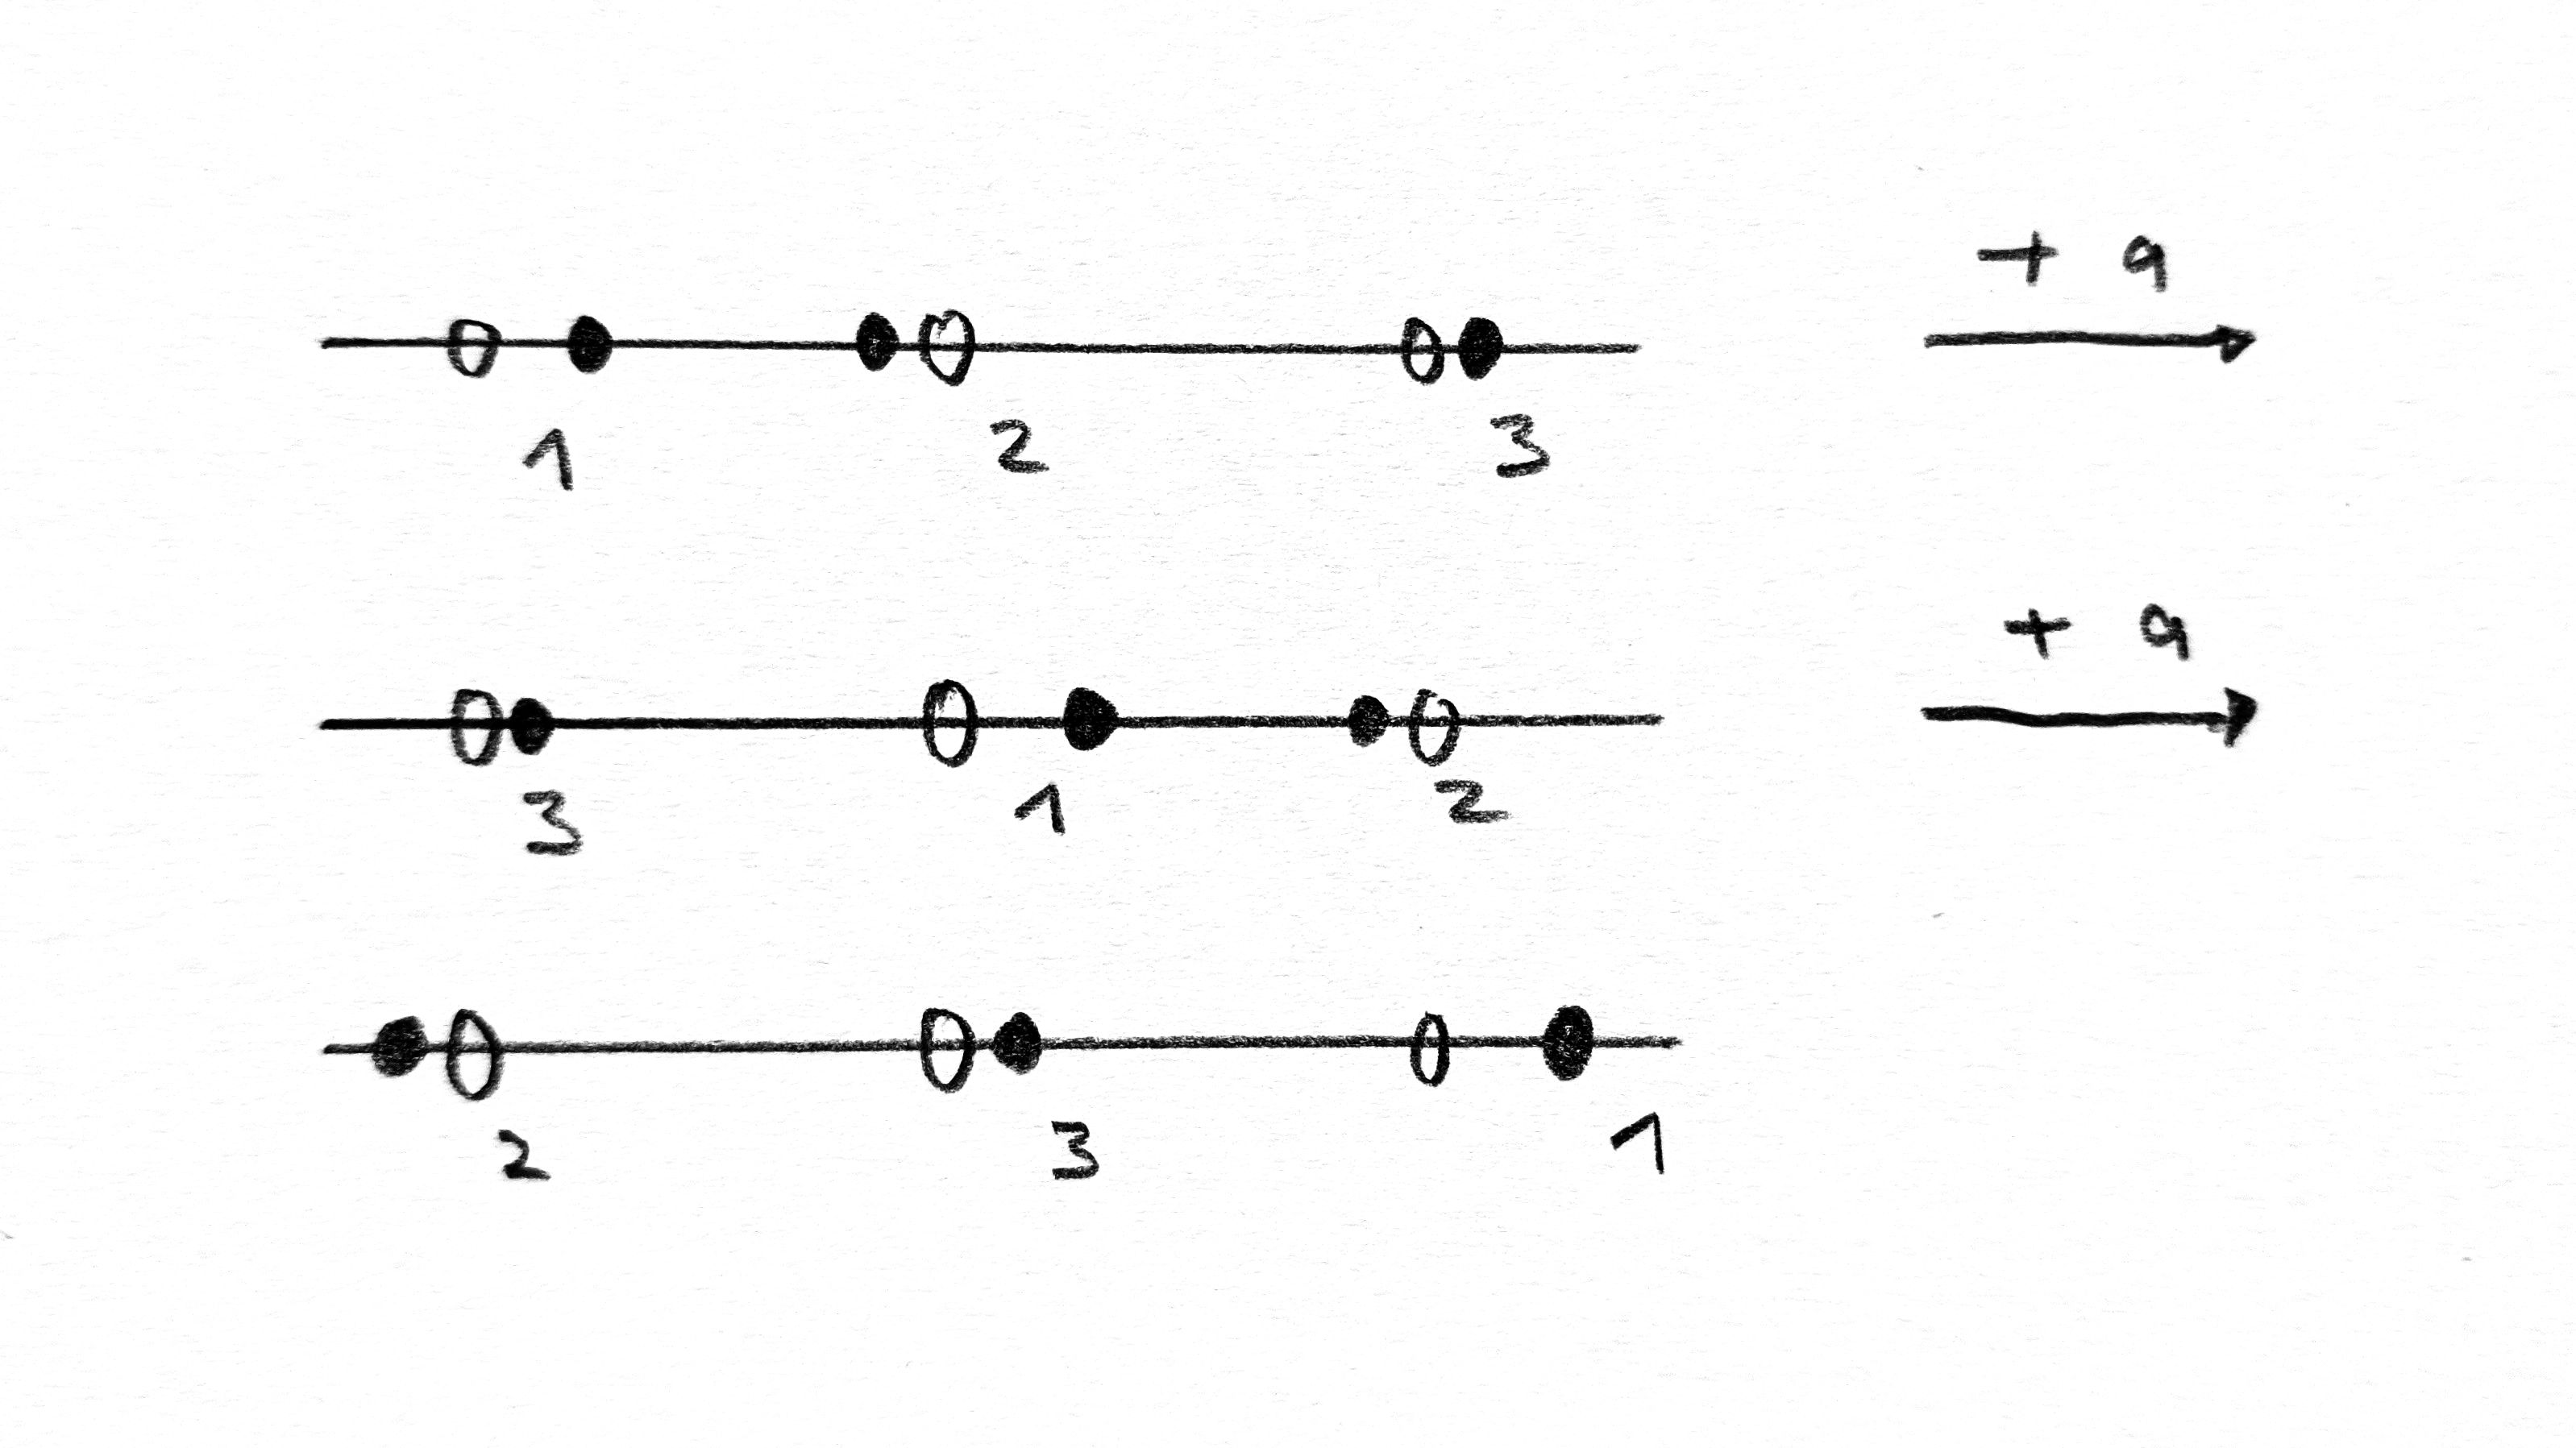
\includegraphics[width=.68\textwidth]{./sketches/permutation1.jpg}
	\caption{A linear chain with three atoms (bullets) displaced from their equilibrium position (open circels). With periodic boundary conditions, the consecutive translation by a lattice vector $a$ induces a permutation of the atoms,~i.\,e.,~$(1, 2 , 3) \to (3, 1, 2) \to (2, 3, 1)$.}
	\label{fig:translation.permutation}
\end{figure}

We can draw two important conclusions from Eq.\,\eqref{eq:translation.permutation} and \eqref{eq:inv.V}. First, the existence of the map $P_{\bf L}$ enables us to write every atomic coordinate ${\bf R}_I$ as
\begin{align}
	{\bf R}_I \equiv {\bf R}_{i {\bf L}} 
		= {\bf R}^0_i + {\bf U}_{i {\bf L}} + {\bf L}~,
	\label{eq:R_iL}
\end{align}
where ${\bf R}^0_i$ labels the position of an equivalent reference atom in the unit cell, ${\bf U}_{i {\bf L}}$ is the displacement of the atom from its equilibrium position, and $\bf L$ is a Bravais vector as before.
We can therefore split the index $I$ into a tuple $I = (i, {\bf L})$,~i.\,e.,~unit cell and lattice point labels.

Second, the harmonic force constants $\Phi_{I \alpha, J \beta}$ can be written as $\Phi_{i {\bf L} \alpha, j {\bf K} \beta}$~, where $\bf L$ and $\b K$ are the Bravais vectors belonging to $I$ and $J$, respectively. From the translational invariance of the potential, Eq.\,\eqref{eq:inv.V}, we see that the force constants have to fulfill
\begin{align}
	\Phi_{i {\bf L} + \b M \alpha, j {\bf K} + \b M \beta} 
		= \Phi_{i {\bf L} \alpha, j {\bf K} \beta}~,
	\label{eq:fc.sym.1}
\end{align}
where $\b M$ again denotes an arbitrary Bravais vector. Using this translational invariance, we can Fourier transform the dynamical matrix defined in Eq.\,\eqref{eq:D},
\begin{align}
	{\rm D}_{i \alpha, j \beta} (\b q) 
		= \sum_{\b L} {\rm e}^{- \im \b q \cdot \b L} {\rm D}_{i \b 0 \alpha, j \b L \beta}
	\label{eq:D(q)}
\end{align}
where we restrict the values of $\b q$ to reside in the first Brillouin zone, thereby transforming the $3N \times 3N$ matrix ${\rm D}_{IJ}$ to one $3n \times 3n$ matrix ${\rm D}_{ij} (\bf q)$ for each~$\b q$, where $n$ is the number of atoms in the primitive unit cell.

\subsubsection{Cyclic Boundary Conditions and Supercell Approximation}
In the previous section, we did not specify the system beyond requiring periodic boundary conditions, and implicitly assumed an infinite crystal in the limit $N \to \infty$ without boundaries. In practice we introduce Born-von Karman cyclic boundary conditions~\cite{born2013atomtheorie}, as already done in Sec.\,\ref{sec:theory.periodic.1} for the description of electronic states, but reintroduce them here in a slightly more general fashion.

We define the boundary conditions for the nuclear problem such that
\begin{align}
	\b R_I + S^i \b A_i = \b R_I \quad\text{for}\quad S^i \in \mathds{Z}~,
	\label{eq:sc.1}
\end{align}
where each ${\bf A}_i$ is a linear combination of the primitive basis vectors $\set{{\bf a}_i}$,
\begin{align}
{\bf A}_i = {\rm M}_{ij}^{\rm sc} {\bf a}_j\quad\text{with } {\rm M}_{ij}^{\rm sc} \in \mathds Z~,
\end{align}
and $\rm M^{\rm sc}$ is a non-singular matrix with integer elements. The space spanned by the $\set{{\bf A}_i}$ is parallelepiped of volume $V_{\rm sc} = N_{\rm sc} \, {\bf a}_1 \cdot ({\bf a}_2 \times {\bf a}_3)$, where $N_{\rm sc} = \det {\rm M}^{\rm sc}$ is the number of unit cells that fit into the enlarged cell, and $V_{\rm uc} = {\bf a}_1 \cdot ({\bf a}_2 \times {\bf a}_3)$ is the unit cell volume. This cell is therefore called \emph{supercell} and we define it such that its midpoint is located at the origin,~i.\,e.,~
\begin{align}
	\mathds V_{\rm sc}
		&= \set{{\bf X} = X^i {\bf A}_i : X^i \in {[-0.5, 0.5)_{\mathds R}}}~.
	\label{eq:supercell}
\end{align}
We therefore denote the matrix ${\rm M}^{\rm sc}$ as the \emph{supercell matrix}.
The vectors \mbox{$\b S = S^i \b A_i$} are the equivalent of the Bravais vectors $\b L$ in a superlattice described by $\set{ \b A_i }$ instead of $\set{ \b a_i}$.
The ideal, infinite crystal is obtained in the limit $N_{\rm sc} \rightarrow \infty$.
From Eq.\,\eqref{eq:sc.1} we see that the force constants become periodic functions in the superlattice,
\begin{align}
	\Phi_{i {\bf L} \alpha, j {\bf K} + \b S \beta} 
		= \Phi_{i {\bf L} \alpha, j {\bf K} \beta} \quad\text{for all}\quad \b S = S^i \b A_i~,
	\label{eq:fc.sym.2}
\end{align}
so that the dynamical matrix in Eq.\,\eqref{eq:D(q)} can be written as a sum over lattice points that are contained in the supercell only,
%\begin{align}
%	{\rm D}_{i \alpha, j \beta} (\b q) 
%		&= \sum_{\b L \in \mathds V_{\rm sc}} 
%			\left( 
%				{\rm e}^{- \im \b q \cdot \b L} {\rm D}_{i \b 0 \alpha, j \b L \beta}
%			+ \sum_{\b S \neq \b 0} {\rm e}^{- \im \b q \cdot (\b L + \b S)} {\rm D}_{i \b 0 \alpha, j \b L \beta}
%			\right)~.
%	\label{eq:D^S(q).1}
%\end{align}
\begin{align}
	{\rm D}_{i \alpha, j \beta} (\b q_{\bf m}) 	
		&= %\frac{N}{N_{\rm sc}} 
	\sum_{\b L \in \mathds V_{\rm sc}} {\rm e}^{- \im \b q_{\bf m} \cdot \b L} {\rm D}_{i \b 0 \alpha, j \b L \beta}~.
	\label{eq:D^S(q).2}
\end{align}
for $\b q_{\b m}$ that fulfill
\begin{align}
	{\bf q_{\b m}} \cdot {\bf A}_i	= 2 \pi m_i \quad\text{with}\quad m_i \in \mathds Z~.
	\label{eq:q.commensurate}
\end{align}
%the summands in the second sum of Eq.\,\eqref{eq:D^S(q).1} interfere constructively and yield a factor $\sum_{\b S}' = N / N_{\rm sc} - 1$. For all other $\b q$, the entire summand becomes negligible in the limit $N \to \infty$ when normalized to the supercell volume.
The $\b q_{\b m}$ that fulfill Eq.\,\eqref{eq:q.commensurate} are called \emph{commensurate} $\b q$-points, as they represent wave numbers that fit into the supercell.
In total there are $N_{\rm sc}$ non-equivalent values of $\bf q_{\b m}$ labelled by ${\bf m} = (m_1, m_2, m_3)$ that can be expressed in terms of the lattice vectors of the reciprocal supercell,
\begin{align}
{\bf B}^i 
= 2 \pi \varepsilon^{ijk} \frac{{\bf A}_j \times {\bf A}_k}{{\bf A}_1 \cdot ({\bf A}_2 \times {\bf A}_3)} ~,
%\label{eq:dft.Bloch.bi}
\end{align}
where $\varepsilon^{ijk}$ denotes the Levi-Civita symbol enforcing the correct ordering of $ijk$. The complete set of $\bf q$-values is
\begin{align}
{\bf q}_{\bf m} 
= \sum_{i=1}^3 m_i {\bf B}^i~,
\label{eq:q_m}
\end{align}
with $m_i \in \mathds Z$ such that $\b q_{\bf m}$ is an element of the first Brillouin zone of the direct lattice.
%For the set of commensurate $\b q$-points, the dynamical matrix is therefore given by
%\begin{align}
%{\rm D}_{i \alpha, j \beta} (\b q_{\bf m}) 	
%	&= %\frac{N}{N_{\rm sc}} 
%	\sum_{\b L \in \mathds V_{\rm sc}} {\rm e}^{- \im \b q_{\bf m} \cdot \b L} {\rm D}_{i \b 0 \alpha, j \b L \beta}~.
%	\label{eq:D^S(q).2}
%\end{align}


\subsubsection{Interpolation to non-commensurate q-points}
The definition of the dynamical matrix in Eq.\,\eqref{eq:D^S(q).2} was formulated for commensurate $\b q$-points $\set{\b q_{\b m}}$,~i.\,e.,~those given in terms of Eq.\,\eqref{eq:q_m}. Evaluating this expression at a non-commensurate value of $\b q$ will, in general, yield a non-hermitian matrix which cannot be used to extract physically sound information about the system. To obtain an \emph{approximated} dynamical matrix at any other, non-commensurate value of $\b q$ within the Brillouin zone, we define an \emph{extended supercell}, 
\begin{align}
	\mathds V_{\rm sc}^{\rm ext}
		&= \set{{\bf X} = X^i {\bf A}_i : X^i \in {[-0.5, 0.5 \boldsymbol{]}_{\mathds R}}}~,
	\label{eq:supercell.extended}
\end{align}
which also contains the lattice points at the positive boundary of the supercell as depicted by open circles in Fig.\,\ref{fig:sketch_supercells}.
\begin{figure}[t]
	\centering
	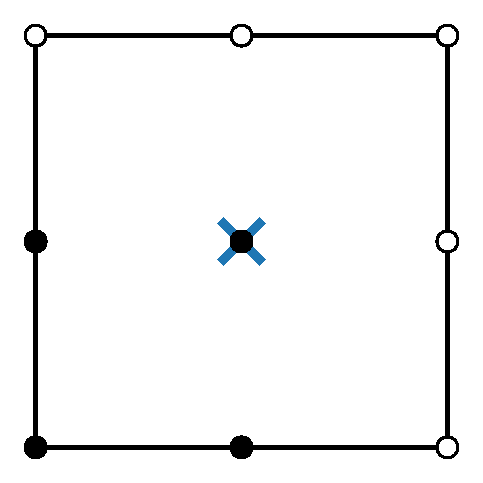
\includegraphics[width=.32\textwidth]{./sketches/2_sc.pdf}
	\hfill
	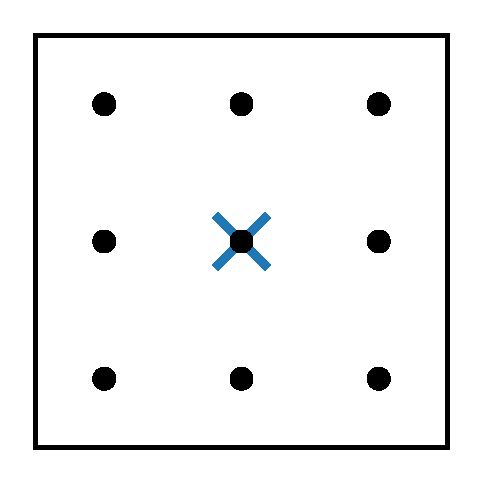
\includegraphics[width=.32\textwidth]{./sketches/3_sc.pdf}
	\hfill
	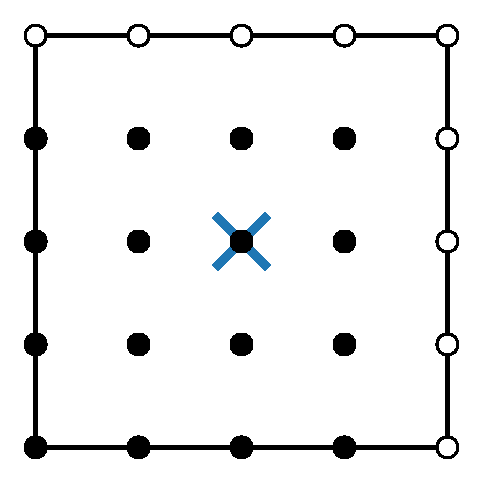
\includegraphics[width=.32\textwidth]{./sketches/4_sc.pdf}
	\caption{Depiction of square supercells with lattice points in the range $[-0.5 A, 0.5 A)$ (bullets $\bullet$), and extended lattice points at the supercell boundary (empty bullets $\circ$), where $A$ is the edge length of the supercell. Blue arrows denote the unit cell vectors, black arrows denote the supercell vectors.}
	\label{fig:sketch_supercells}
\end{figure}
These lattice points are included in the Fourier series with an appropriate weight $w_{\b L}$ that accounts for double counting of lattice points that are separated by a linear combination of supercell lattice vectors~\cite{Parlinski1997}. Furthermore, we use a minimal image convention (MIC) between the atoms $(i, \b 0)$ and $(j, \b L)$,~i.\,e.,~for each pair we use an equivalent lattice point $\b L'$ within the extended supercell which depends on $(i, j, \b L)$ such that
\begin{align}
	- \b R_{i \b 0 } + \b R_{j \b 0} + \b L' \in V_{\rm sc}^{\rm ext}~.
	\label{eq:L'}
\end{align}
In total we define
\begin{align}
	{\rm D}_{i \alpha, j \beta} (\b q) 	
		&= %\frac{N}{N_{\rm sc}} 
		\sum_{\b L \in \mathds V_{\rm sc}^{\rm ext}} 
			w_{\b L}
		{\rm e}^{- \im \b q \cdot \b L'} {\rm D}_{i \b 0 \alpha, j \b L \beta}~.
	\label{eq:D_Parlinski}
\end{align}
We note that the dynamical matrix elements defined by Eq.\,\eqref{eq:D_Parlinski} differ from the ones found in Ref.~\cite{Parlinski1997} by a phase factor ${\rm e}^{\im \b q \cdot (\b R_i^0 - \b R_j^0)}$, which is typical when the discussion is performed from a lattice-wave ansatz to solve the equations of motion~\cite[p. 298]{BornHuang}.

For each $\b q$, ${\rm D} (\b q)$ is a hermitian $3n \times 3n$ matrix in the indices $(i \alpha, j \beta)$ and will therefore yield $3n$ real eigenvalues and $3n$ complex, orthogonal eigenvectors, which denote in accordance with Eq.\,\eqref{eq:sum_D_IJ}
\begin{align}
\sum_{j \beta} {\rm D}_{i \alpha, j \beta} (\b q) e_{j \beta} (\b q , b)
= \omega^2 \, (\b q, b) e_{i \alpha} (\b q , b)~,
\label{eq:D_ij(q)w}
\end{align}
where the \emph{band index} $b$ is used to discern the $3n$ \emph{branches} at each $\b q$. Using the combined index $s = (\b q, b)$, the notation becomes similar to the non-periodic case with $3N_{\rm sc} N_{\rm uc}$ degrees of freedom, only that the eigenvectors $\b e_{s = (\b q, n)}$ can be complex valued instead of strictly real.
\REM{This is Born conventions. Togo and Parlinski use extra phase factor ${\rm e}^{\im \b q \cdot (\b R_i^0 - \b R_j^0)}$ that alters the eigenvectors but not the frequencies.}

\subsubsection{Ledermann's Theorem}

%As we will be interested in the eigenvalues and eigenvectors of the dynamical matrices $\rm D ({\b q})$, the prefactor $N/N_{\rm sc}$ can be neglected in the following.

\REM{for $\b q = \b q_{\b m}$ D is exact up to boundary effects (?!), nevertheless one can interpolate -> Fourier interpolation}
\REM{Alternative: Use effective cutoff of $\Phi$}
\REM{Effective cutoff -> effect on spectrum, Maradudin, Ledermann}

% Equation~\eqref{eq:D^S(q).2} will in general not be hermitian in $(i \alpha, j \beta)$

\subsubsection{Finite Differences}
The force constants can be obtained from first-order derivatives of the potential-energy surface,~i.\,e.,~the forces, by rewriting the second derivative in terms of a finite difference expression,
\begin{align}
	\Phi_{I \alpha, J \beta}
		= \left.\frac{\partial^{2} \mathcal{V}(\mathbf{R})}{\partial R_{I}^{\alpha} \partial R_{J}^{\beta}}\right|_{\mathbf{R}^{0}}
		= - \frac{\partial}{\partial R_I^\alpha} F_{J, \beta}
		= - \lim_{\epsilon \to 0}
			\frac{F_{J, \beta} (\set{\b R': R^{\prime \beta}_I = R^{\beta}_I + \epsilon )}}{\epsilon}
		~.
\label{eq:FC2_finite}
\end{align}
In practice, atom $J$ is displaced by a small but finite displacement $\epsilon$ in the direction $\beta$, and the force on all other atoms is recorded. By performing the displacement in all $3N$ degrees of freedom, the $3N \times 3N$ forces can be arranges in a matrix $F_{[3N \times 3N]}$, and the displacements can be arranged in a matrix $U_{[3N \times 3N]} = \epsilon \mathds 1_{[3N \times 3N]}$. The $3N \times 3N$ force-constants matrix $\Phi$ is obtained by the trivial matrix inversion
\begin{align}
F &= - H U = - \epsilon \Phi \mathds 1\\
\implies
\Phi &= - \frac{1}{\epsilon} F \mathds 1~.
\end{align}
%\begin{align}
%	F &= - H U \\
%	\implies
%	H &= - U^{+} F \\
%	F &= \begin{pmatrix} \b F_1, & \cdots, & \b F_{3N} \end{pmatrix}
%\end{align}
If $M > 3N$ displacements are used,~e.\,g.,~because positive and negative displacements $\pm \epsilon$ are used, the force constants can be obtained by solving an overdetermined linear equation of the kind
\begin{align}
	F_{[3N \times M]} &= - \Phi_{[3N \times 3N]} U_{[3N \times M]} \\
	\implies
	\Phi &= - U^{+} F~,
%	F &= \begin{pmatrix} \b F_1, & \cdots, & \b F_{3N} \end{pmatrix}
\end{align}
where $U^{+}$ denotes the Moore-Penrose pseudo inverse of the displacement matrix $U$~\CITE{pseudoinverse}.
\CITE{Parlinski, Togo}

In practice, the number of required force calculations can be reduced by considering the spacegroup symmetry of the crystal. This can be achieved in two ways: First, the symmetry can be used to identify the set of inequivalent displacements from which all other forces can be reconstructed. Second, the symmetry can be used to reduce the forceconstant matrix to an irreducible basis.

\REM{Symmetry: 2 ways: i) construct full $F$ from a reduced set of displacements, ii) reduce $H$ to reduces/irreducible representation like original Parlinski article.}

\subsection{Harmonic Sampling}

\subsection{Molecular Dynamics}
The classical limit of the nuclear Schr\"odinger equation~\eqref{eq:BOSE} is usually performed by writing the nuclear wavefunction $\chi_s ({\bf R}, t)$ in terms of a real amplitude $A_s({\bf R}, t)$ and a \emph{classical action function} $S_s({\bf R}, t)$~\cite{Dirac1981,Landau2013,Marx2009}
\begin{align}
	\chi_s({\bf R}, t) = A_s({\bf R}, t) \, {\rm e}^{\frac{\im}{\hbar} S_s({\bf R}, t)}~.
	\label{eq:class.1}
\end{align}
The Schr\"odinger equation then yields a set of differential equations for $A_s$ and $S_s$ that, in the limit $\hbar \to 0$, go over to a \emph{Hamilton-Jacobi} equation for $S_s$,~i.\,e.,~
\begin{align}
  \frac{\partial S_s}{\partial t} + \mathcal H \left({\bf R}, {\bf P}\right)
  = 0~,
  \label{eq:HamiltonJacobi}
\end{align}
where ${\bf P} = ({\bf P}_1, \ldots) \equiv ({\bf \nabla}_1 S_s, \ldots)$ denotes the conjugate momenta and $\mathcal H$ is the \emph{classical} Hamilton function corresponding the to the operator in Eq.\,\eqref{eq:BOSE}, from which the equations of motion for the nuclei can be obtained:
\begin{align}
  \dot{{\bf P}}_I 
    = -\frac{\partial \mathcal H}{\partial {\bf R}_I}
    \quad\implies\quad M_I \ddot{\bf R}_I
    = -\frac{\partial \mathcal V}{\partial {\bf R}_I}~.
    % \equiv - {\bf F}_I~.
\end{align}
The negative gradient of the Born-Oppenheimer potential, 
$-\partial \mathcal V / \partial {\bf R}_I$ is the force ${\bf F}_I$ acting on atom $I$ which can be obtained via the Hellmann-Feynmann theorem,~cf.~Sec.\,\ref{sec:HellmannFeynman}.

An alternative viewpoint that is more instructive can be taken by invoking the \emph{Ehrenfest theorem}~\cite{Ehrenfest1927,Basdevant2007}. The statement is that
\begin{align}
  \frac{\d}{\d t} \left\langle {\bf P}_I \right\rangle_{\chi_s}
    = \left\langle
      - \frac{\partial \mathcal{V}}{\partial {\bf R}_I}
    \right\rangle_{\chi_s}~,
  \label{eq:ehrenfest.de1}
\end{align}
where $\langle \cdot \rangle_{\chi_s}$ denotes an expectation value taken with respect to the state $\chi_s$. This expression differs only slightly from the classical counterpart, which would read
\begin{align}
\frac{\d}{\d t} \left\langle {\bf P}_I \right\rangle
= \left.
- \frac{\partial \mathcal{V}}{\partial {\bf R}_I}
\right\vert_{{\bf R} = \langle {\bf R} \rangle}~.
\label{eq:ehrenfest.de2}
\end{align}
The difference comes from the fact that, in general,
\begin{align}
  \delta f  \equiv 
  f \bm ( \langle x \rangle \bm{)} 
  - 
  \bm{\langle} f (x) \bm{\rangle}
  \neq 0
  ~,
  \label{eq:ehrenfest.delta1}
\end{align}
where $x = {\bf R}_I$ denotes the space coordinate for notional simplicity, $f$ is some function of the observable $x$, and $\delta f$ measures the difference between the classical and the quantum expectation value. Ehrenfest's argument is that this difference becomes negligible when the state is sufficiently peaked around some value $x_0$. Expanding $f$ around the expectation value of $x$, $x_0 \equiv \langle x \rangle$, we have
\begin{align}
  f(x) = f \bm ( \langle x \rangle \bm{)}  
    + (x - \langle x \rangle) \, f' \bm ( \langle x \rangle \bm{)}
    + \frac{1}{2} (x - \langle x \rangle)^2 \, f'' \bm ( \langle x \rangle \bm{)}
    + \cdots~.
  \label{eq:ehrenfest.f2}
\end{align}
It follows that the $f'$ term vanishes when the expectation value is taken, and
\begin{align}
\langle f(x) \rangle 
  = f \bm ( \langle x \rangle \bm{)}  
    + \frac{1}{2} \Delta x^2 f'' \bm ( \langle x \rangle \bm{)}
    + \cdots~,
\label{eq:ehrenfest.f3}
\end{align}
where $\Delta x^2 = \bm{\langle} (x - \langle x \rangle)^2 \bm{\rangle}$ measures the variance of the underlying distribution,~i.\,e.~the width of the wavepacket. The relative error between the classical and quantum expectation value is readily computed to be
\begin{align}
  \left\lvert \frac{\delta f}{f \bm ( \langle x \rangle \bm{)}} \right\rvert
  = \frac{1}{2} \Delta x^2 \left\lvert \frac{f'' \bm ( \langle x \rangle \bm{)}}{f \bm ( \langle x \rangle \bm{)}} \right\rvert
+ \mathcal{O}(\Delta x^3)~.
  \label{eq:ehrenfest.delta2}
\end{align}
This estimation holds in general for any observable $f$.
By crudely estimating the dimension of the wavepacket in terms of the thermal de Broglie-wavelength, we find
\begin{align}
  \Delta x^2 
    \sim \left( \frac{h}{P} \right)^2
    \sim \frac{h^2}{MT}~,
  \label{eq:ehrenfest:dimension}
\end{align}
which gives support to the intuitive assumption that we can expect the classical limit to work better the heavier the atoms and the higher the temperature.
Let us now set $f(x) \hat = -\partial \mathcal V / \partial {\bf R}_I$, then another important conclusion can be drawn from Eq.\,\eqref{eq:ehrenfest.delta2}: For a harmonic potential $\mathcal V ({\bf R}) = \mathcal V^{(2)} ({\bf R})$, where derivatives higher than second order vanish, the classical and quantum mechanical expectation values \emph{always coincide}. The quantum mechanical expectation value of position will therefore evolve in the same time-periodic fashion as a classical particle in a harmonic well.

\REM{this approach can only be validated by computing observables and compare the results. One can safely say that this approach has been used successfully in a plethora of studies, while additional care must be taken at low temperature and/or systems with light atoms, especially hydrogen-bonded systems~\CITE{MD-Review?,MarklandCeriotti,Litman,pHexperiment}.}

\subsubsection{Thermodynamic Ensembles and Thermostats}
\subsubsection{Finite Temperature Equations of State and Lattice Expansion}
\subsubsection{Mode Projection}
\subsubsection{Approximative Anharmonic Methods}

\subsection{Heat Transport}
\subsubsection{Fluctuation Dissipation Theorem}
\subsubsection{Green and Kubo}
\subsubsection{Ab initio Virial Heat Flux}
\subsubsection{Ab initio Green Kubo}
% %
% \chapter{Heat Transport}
% \label{chp:heat_transport}
\epigraph{\singlespacing \it ``It seems there is no problem in modern physics for which there are on record as many false starts, and as many theories which overlook some essential feature, as in the problem of the thermal conductivity of [electrically] non-conducting crystals.''}{R.~Peierls, 1960~\cite{Peierls1960}}

As this quote by Rudolf Peierls exemplifies, developing a microscopic theory for heat transport in dielectric crystals was a long-standing problem for solid-state physics in the 20th century. Early attempts to explain this phenomenon sparked by experiments conducted by Eucken comprise those by Einstein, Debye, and Born and von Karman in the early 1910s~\cite{Eucken.1911,Einstein.1911,Debye.1912,Cahill.1988}. However, they failed to explain the experimental findings (Einstein), or could only provide qualitative understanding (Debye). One key insight by Debye missing in the earlier attempt by Einstein is the notion of a \emph{phonon gas},~i.\,e.,~that the collective excitations of the nuclear degrees of freedom show qualitatively similar behavior as molecules in a gas. It was in 1929 that Peierls himself contributed a model for heat transport in solids that was able to explain key experimental findings such as the $1/T$ dependence of a material's thermal conductivity at elevated temperatures, which he could achieve by computing three-phonon scattering due to anharmonic terms in the potential-energy surface~\cite{Peierls.1929}. It took another 80 years until this approach led to the development of a fully \emph{ab initio} computational approach by Broido and coworkers in 2007~\cite{Broido.2007}, using the method of Boltzmann transport equation pioneered by Peierls and further developed in the meantime~\cite{Omini.1996,Omini.1997,Broido.2005}. By the time of writing this work, Boltzmann transport theory is the established way to compute thermal transport properties of dielectric crystals from first principles, and many new, more refined approaches have been developed in recent years~\cite{Feng.2016,Xia.2018,Ravichandran.2018,Simoncelli.2019}.

\newthought{However, Boltzmann transport theory always relies on the phonon gas model} and treats phonon-phonon interactions as perturbative effects due to low-order anharmonic corrections to the potential-energy surface. When dealing with strongly anharmonic materials, this perturbative treatment becomes more and more cumbersome, and sometimes even unjustified, as we will discuss in more detail later. In this chapter, we therefore review heat transport in solids in the framework of Green-Kubo theory without treating the nuclear dynamics as a phonon gas~ \cite{Green.1952,Kubo1957a,Kubo1957b,Helfand.1960,Hardy.1963}.

\section{Introduction}
\label{sec:thermal_conductivity}
Conductive heat transport is the phenomenon of vibrational energy traversing a material when a temperature gradient is applied. As first described by Joseph Fourier in the early 19th century, the heat flux $\b J$ resulting from a stationary temperature gradient $\nabla T$ is directly proportional to this gradient~\cite{Fourier1878}. The proportionality constant is second-rank tensor denoted by $\kappa$ and called the \emph{thermal conductivity}. The defining equation,
\begin{align}
  \b J = - \kappa \nabla T~,
  \label{eq:Fourier}
\end{align}
is called \emph{Fourier's law}. The sign convention is such that the heat flows from ``hot to cold'' in accordance with the second law of thermodynamics. The regime where Eq.\,\eqref{eq:Fourier} is valid is called the \emph{diffusive} regime, as it holds when the temperature gradient is small on microscopic scale, and the sample size is big enough so that boundary effects are negligible~\cite{Kapitza1941a,Antidormi2020}.

It is evident from Eq.\,\eqref{eq:Fourier} that the thermal conductivity $\kappa$ is an explicitly non-equilibrium quantity. As such, it can be related to equilibrium fluctuations by means of the \emph{fluctuation-dissipation theorem}~\cite{Einstein1905a,Nyquist.1928,Callen.1951,Kubo1957a}, resulting in the famous Green-Kubo formula~\cite{Green.1952,Kubo1957b},
\begin{align}
  \kappa^{\alpha \beta} = \frac{V}{k_{\rm B} T^2} \int_{0}^{\infty} \d t ~
    \braket{J^\alpha (t) J^\beta(0)}_{\rm eq}~.
  \label{eq:GreenKubo_0}
\end{align}
This formula relates the temporal fluctuations of the macroscopic heat flux $\b J (t)$ as given by an equilibrium ensemble average of the autocorrelation function, $\braket{J^\alpha (t) J^\beta(0)}_{\rm eq}$, to the associated transport coefficient $\kappa^{\alpha \beta}$, where $\alpha$ and $\beta$ denote the respective Cartesian components. It is however \emph{a priori} unclear how a microscopic description of the appearing quantities can be obtained. To tackle this question in full, we 
%\mscomment{``we'': you or someone else?}
%\FK{``closely following Baroni and coworkers in Ref.\,\cite{Baroni2020a}''. Clarify how many dots I connected}
first show how the Kubo formula emerges in the framework of linear response theory, closely following Baroni and coworkers in Ref.\,\cite{Baroni2020a}. We then present how a microscopic description of heat in terms of a thermal energy density and an associated, locally conserved current follows, before reviewing the necessary steps to define an \emph{ab initio} heat flux~\cite{Carbogno.2016}.



\section{Linear response theory}
The aim of linear response theory is to compute the expectation value of a phase-space observable $B (\Gamma)$ in a system characterized by the many-body Hamiltonian $\mathcal H^0 (\Gamma)$ in presence of an external perturbation $\mathcal H' (\Gamma, t)$ driving the system out of equilibrium, where $\Gamma = \set{\b R, \b P}$ is a shorthand for a point in phase space.\footnote{The notation used in this chapter was introduced in Sec.\,\ref{sec:statistical-mechanics}.}
The full Hamiltonian is written as
\begin{align}
  \mathcal H (\Gamma, t)
   = \mathcal H^0 (\Gamma) + \mathcal H' (\Gamma, t)~,
  \label{eq:lr.H}
\end{align}
where the perturbation $\mathcal H' (\Gamma, t)$ is usually given as
%
\begin{align}
  \mathcal H' (\Gamma, t)= A (\Gamma) F(t)~,
  \label{eq:lr.H_AF}
\end{align}
%
with $A(\Gamma)$ representing an operator coupling to the system, and $F(t)$ is an explicitly time-dependent force function.

The task is to compute the expectation value of $B$ as defined in Eq.\,\eqref{eq:phase.space.average},
%
\begin{align}
  \braket{B (t)}
    = \int \d \Gamma ~ B (\Gamma) f(\Gamma, t)~,
  \label{eq:lr.B.1}
\end{align}
%
in the presence of the perturbation $\mathcal H'$, where $f (\Gamma)$ is the canonical distribution function characterizing the statistical ensemble at inverse temperature $\beta$.

\newthought{In the limit of linear response},~i.\,e.,~in the limit of a small \emph{external} perturbation $\mathcal H'$,\footnote{This is not to be confused with a perturbation expansion of $\mathcal H^0$, which is treated exactly here.} the expected response of the phase space observable $B$ to the system Hamiltonian defined in Eq.\,\eqref{eq:lr.H} is given as
%
\begin{align}
\braket{B (t)}
%    &= \int \d \Gamma ~  B (\Gamma) \Delta f (\Gamma, t) \\
%    &= - \beta \int_{-\infty}^t 
%      \int \d \Gamma ~  
%       B (\Gamma) \, {\rm e}^{-\im \mathcal L^0 (t - t')} \dot{A}(\Gamma)
%       f^0(\Gamma) F(t') ~ \d t' \\
    = - \beta \int_{-\infty}^t 
      \braket{B(\Gamma_t) \dot{A} (\Gamma_{t'})}_{0} F(t') ~ \d t'~,
  \label{eq:lr.dB}
\end{align}
%
where $\braket{\cdot}_{0}$ denotes a phase-space average with respect to the unperturbed canonical distribution function
%
\begin{align}
  f^0 (\Gamma) 
    = \frac{1}{\mathcal{Z}^0} {\rm e}^{- \beta \mathcal H^0 (\Gamma)}~,
  \label{eq:lr.f0}
\end{align}
where the partition sum $\mathcal{Z}_0$ normalizes the phase-space integral \mbox{$\int \d \Gamma f^0 (\Gamma)$}.
The notation implies that for each phase-space point $\Gamma$ in the ensemble, $B (\Gamma)$ and $\dot{A} (\Gamma)$, the total time derivative of $A (\Gamma)$, are evaluated at phase-space points separated in time by $t-t'$~\cite[p.\,498]{Tuckerman}.
%it was used that $a(t) = {\rm e}^{\im \mathcal L^0 t} a(0) = a(0) {\rm e}^{-\im \mathcal L^0 t}$, and  as before. 
%It is evident from this equation that the time propagation of the observables $\dot {A}$ and $B$ 
The time propagation of phase-space points is generated by $\mathcal H^0$ and therefore given by Hamilton's equations of motion with conserved energy as defined in Eq.\,\eqref{eq:stat.eom}. The phase-space average $\braket{\cdot}_{0}$ on the other hand corresponds to a canonical ensemble average with respect to the distribution function $f^0$ defined in Eq.\,\eqref{eq:lr.f0}. A derivation of Eq.\,\eqref{eq:lr.dB} is given in Chp.\,\ref{app:linear_response} in the appendix.



\subsection{Locally conserved densities and currents}
Macroscopic properties of matter are often \emph{extensive},~i.\,e.,~they scale with the system size, and can be described by a locally conserved \emph{density}~\cite{Baroni2020a}. Taking the general property $A$ represented by the phase-space observable $A(\Gamma_t)$ evaluated at a time $t$ as an example, we define
\begin{align}
  A (\Gamma_t) = \int_V a (\b r, \Gamma_t) \, \d^3 r~,
  \label{eq:lr.A}
\end{align}
where $a(\b r, \Gamma_t)$ is a suitably chosen \emph{local density} associated with the observable $A$. The notation $\Gamma_t$ was introduced in Sec.\,\ref{sec:phase_space} to highlight that $A$ is implicitly time-dependent because the phase-space configuration $\Gamma$ evolves in time.
%When no ambiguity arises, we can therefore just write $a (\b r, t)$.\footnote{
%	Notation for phase-space functions $f (\Gamma)$:
%	\begin{align*}
%	f(t) &\equiv f(\Gamma (t)) \\
%	\frac{\partial f}{\partial t} &= \frac{\d f (\Gamma (t))}{\d t} \equiv \dot{f}(t)
%	\end{align*}
%}
The locally conserved density fulfills a continuity equation
\begin{align}
  \partial_t \, a(\b r, \Gamma_t) = - \b \nabla \cdot \b j (\b r, \Gamma_t)~,
  \label{eq:lr.continuity.1}
\end{align}
where $\b j (\b r, \Gamma_t)$ is the associated local current. From the local current, the macroscopic flux is obtained by spatially averaging over the system volume,
\begin{align}
  \b J (\Gamma_t)
    = \frac{1}{V} \int_V \d^3 r ~ \b j (\b r, \Gamma_t)~.
  \label{eq:lr.J(t)}
\end{align}
Likewise we formulate a local version of the perturbing Hamiltonian initially defined in Eq.\,\eqref{eq:lr.H_AF},
\begin{align}
	\mathcal H' (\Gamma_t, t) = \int \d^3 r ~ a (\b r, \Gamma_t) v(\b r, t)~,
	\label{eq:lr.H'}
\end{align}
where $a(\b r, \Gamma_t)$ represents the density of interest as introduced above, and $v(\b r, t)$ is the local driving force coupling to the system via the density $a (\b r, \Gamma_t)$.

The local version of the linear-response formula given in Eq.\,\eqref{eq:lr.dB} for the expectation value of a given local flux $\bf j$ at time $t$ reads:\footnote{Take \mbox{$B \equiv \b J$} with $\braket{B} \equiv \braket{\b J} = 0$~.}
\begin{align}
%j^\alpha (\b r , t) 
%	& \equiv 
\braket{j^\alpha (\b r, t)}
	&= - \beta \int_{-\infty}^{t} \d t' \int_V \d^3 r' ~ \braket{
			j^\alpha (\b r, \Gamma_t) \dot{a} (\b r', \Gamma_{t'})
		}_0 v (\b r', t')~.
	\label{eq:lr.ja.1}
\end{align}
The time derivative of the density can be eliminated by using the continuity equation~\eqref{eq:lr.continuity.1}, $\dot a = - \partial'_\beta j^\beta$ where $\partial'_\beta = \partial/\partial r^{\prime \beta}$, and integrating by parts, so that
\begin{align}
\braket{j^\alpha (\b r , t) }
&= - \beta \int_{-\infty}^{t} \d t' \int_V \d^3 r' ~ \braket{
	j^\alpha (\b r, \Gamma_t) j^\beta (\b r', \Gamma_{t'})
}_0 \partial'_\beta v (\b r', t')~,
\label{eq:lr.ja.2}
\end{align}
where a boundary term was neglected.\footnote{Boundary terms scale proportional to the surface of the integration volume and therefore become negligible in the thermodynamic limit $V \to \infty$.}
If we now assume the external driving force $v (\b r, t)$ to be constant in time and linearly varying in space such that
\begin{align}
	\partial_\beta v (\b r, t) \equiv v_\beta~,
	\label{eq:lr.force}
\end{align}
and spatially average over Eq.\,\eqref{eq:lr.ja.2} with $\frac{1}{V} \int_V \d^3 r$, we arrive at
% \REM{check sign}: there is a double minus: i) continuity equation, ii) integration by parts. correct?
\begin{align}
	J^\alpha 
	\equiv \braket{J^\alpha}
		&= -\beta V \int_{0}^{\infty} 
		\d t
		\braket{
		J^\alpha (\Gamma_t) J^\beta (\Gamma_{0})
	}_0 
	v_\beta~,
	\label{eq:lr.J}
\end{align}
where the stationarity in time was used to shift the lower bound of the integral to $t=0$.
This resembles the well-known macroscopic transport equation~\cite{Onsager1931a}
\begin{align}
	J^\alpha =  L^{\alpha \beta} F_\beta~,
		\label{eq:lr.LF}
\end{align}
where we identify
\begin{align}
	L^{\alpha \beta}
		= \frac{V}{k_{\rm B}} \int_{0}^{\infty} 
		\d t \braket{J^\alpha (\Gamma_t) J^\beta (\Gamma_{0})}_0 ~,
	\label{eq:lr.L}
\end{align}
and
\begin{align}
	F_\beta
		= - \frac{v_\beta}{T}~.
	\label{eq:lr.F}
\end{align}
Here, $J^\alpha$ is the macroscopic generalized current associated with the extensive property $A$, $F_\beta$ is the thermodynamic force, and $L^{\alpha \beta}$ is the associated conductance tensor~\cite{Onsager1931a,Baroni2020a}.

\section{Thermal conductivity}
\label{sec:Thermal.Conductivity}
After this general exposition, let us now look at the example of the total energy of the system and its associated energy density,
\begin{align}
	E = \int_V \d^3 r ~ e(\b r)~.
	\label{eq:lr.E}
\end{align}
We are interested in the occuring flux in the presence of an inhomogeneous temperature, $T(\b r) = T + \Delta T(\b r)$, which couples linearly to the energy density  $e (\b r)$, so that\footnote{$E$ and $\mathcal H(\Gamma)$ are related by $E = \braket{\mathcal H}$. The same holds for the occurring densities $e(\b r)$ and $e (\b r, \Gamma)$.}\footnote{The situation can viewed as a \emph{stationary nonequilibrium state}. The general theory has been worked out by McLennan~\cite{Mclennan.1959,Mclennan.1960}. See also the discussion by Zwanzig in Ref.~\cite{Zwanzig.1965}.}
\begin{align}
	\mathcal H (\Gamma) = \frac{1}{T} \int \d^3 r ~ T (\b r) e(\b r, \Gamma) 
		\equiv \mathcal H^0 (\Gamma) + \mathcal H' (\Gamma)~,
\end{align}
with
\begin{align}
	\mathcal H' (\Gamma) = \frac{1}{T} \int \d^3 r ~ \Delta T (\b r) e(\b r, \Gamma)~.
	\label{eq:lr.Hp.temp}
\end{align}
As earlier in Eq.\,\eqref{eq:lr.force}, we assume $\Delta T(\b r)$ to vary linearly in space, so that the thermodynamic force is given by
\begin{align}
	v_\beta = \frac{1}{T} \partial_\beta T (\b r) 
		\stackrel{\eqref{eq:lr.F}}{\implies}
	F_\beta = - \frac{1}{T^2} (\b \nabla T)_\beta ~.
	\label{eq:lr.F.temp}
\end{align}
Using the general transport equation defined in Eq.\,\ref{eq:lr.LF} with the conductance given by Eq.\,\eqref{eq:lr.L} and $F$ as defined above, we obtain
\begin{align}
	J^\alpha 
		&= - \kappa^{\alpha \beta} (\b \nabla T)_\beta~,
	\label{eq:lr.J.2}
\end{align}
where $\kappa^{\alpha \beta}$ denotes the \emph{thermal conductivity tensor} defined as
\begin{align}
	\kappa^{\alpha \beta}
		&=
		\frac{V}{k_{\rm B} T^2} \int_{0}^{\infty} 
		\d t \braket{J^\alpha (\Gamma_t) J^\beta (\Gamma_{0})}_0 ~,
	\label{eq:GreenKubo}
\end{align}
that is, the Green-Kubo formula for the thermal conductivity $\kappa$.

\section{Heat flux definition}
In order to evaluate the thermal conductivity by means of the Green-Kubo formula, Eq.\,\eqref{eq:GreenKubo}, the  heat flux observable $\b J (t)$ needs to be defined.\footnote{From now on, all time dependence is to be understood as the implicit time dependence of phase-space observables on the time evolution of a phase-space point, $f(t) = f(\Gamma_t)$.} We do so by starting from the continuity equation again,
\begin{align}
	\dot{e} (\b r) = - \b \nabla \cdot \b j (\b r)
	\label{eq:hf.cont}
\end{align}
and perform a Fourier transform in space defined by the pair of equations
\begin{align}
	e(\b r) 
		&= \int \d^3 q ~ e(\b q) \, {\rm e}^{\im \b q \cdot \b r} ~,
		\label{eq:hf.ft.r} \\
	\Leftrightarrow
	e(\b q) 
		&= \frac{1}{V} \int \d^3 r ~ e(\b r) \, {\rm e}^{-\im \b q \cdot \b r} ~,
	\label{eq:hf.ft.2}
\end{align}
so that the continuity equation can be rewritten for the Fourier components as
\begin{align}
	\dot{e} (\b q)
		= - \im \b q \cdot \b j (\b q)~.
	\label{eq:hf.ft.cont.q}
\end{align}
We split the total current into a longitudinal, heat-carrying component $\b j_{\parallel}$ and a transverse current $\b j_{\perp}$,
\begin{align}
	\b j = \frac{\b q}{q} j_{\parallel} + \b j_{\perp} \quad\text{where}\quad \b q \cdot \b j_{\perp} = 0~,
\end{align}
so that
\begin{align}
	\b j_{\parallel} (\b q)
		= \im \frac{\b q}{q^2} \dot{e} (\b q)~.
  \label{eq:hf.j.parallel}
\end{align}
As before, the macroscopic heat flux is given by a spatial average of the (longitudinal) current,
\begin{align}
	\b J = \frac{1}{V} \int \d^3 r ~ \b j_{\parallel} (\b r) = \b j_{\parallel} (\b q \to 0)~,
	\label{eq:hf.J.1}
\end{align}
where it was used that, by definition of the Fourier transform, the integral over the system volume equals the long wavelength limit of the current in reciprocal space. The long wavelength limit for the time derivative of the local energy density can be obtained by Taylor expanding in $\b q$
\begin{align}
	\dot{e} (\b q) 
		= \lim_{\b q \to 0} \int \d^3 r \left(\cancel{1} - \im \b q \cdot \b r + (\b q \cdot \b r)^2 + \cdots \right) \dot{e} (\b r)~,
	\label{eq:hf.e.lw}
\end{align}
where the first term in the expansion is excluded since the total energy $E$ is conserved in time.\footnote{Using the  Leibniz rule,
\begin{align*}
	\int \d^3 r \, \dot{e} (\b r) = \frac{\d}{\d t} \int \d^3 r \, e (\b r) = \frac{\d}{\d t} E = 0~.
\end{align*}
}
After multiplying $\dot e$ with $\im \b q / q^2$ according to Eq.\,\eqref{eq:hf.j.parallel} and taking the $\b q \to 0$ limit, we obtain
\begin{align}
	\b J (t) 
		= \frac{1}{V} \int \d^3 r ~ \b r \, \dot{e} (\b r, t)
		= \frac{1}{V} \frac{\d}{\d t} \int \d^3 r ~ \b r \, e (\b r, t)
	~,
	\label{eq:hf.J}
\end{align}
i.\,e.,~the heat flux is given as the first moment of the time derivative of the local energy density. Alternatively, one can view the heat flux as the time derivative of the energy barycenter by moving the time derivative outside the integral.

In force-field approaches, it is common to adopt the latter approach and split the energy density into atomic contributions $E = \sum_I E_I$ as
\begin{align}
	e (\b r, t ) = \sum_I E_I (t) \delta (\b r - \b R_I (t))~.
	\label{eq:hf.e.atomic}
\end{align}
The heat flux is then given by~\cite{Helfand.1960}
\begin{align}
	\b J (t) 
		= \frac{1}{V} \frac{\d}{\d t} \sum_I E_I(t) \b R_I(t)
		% = \frac{1}{V} \sum_I \dot{E}_I (t) \b R_I (t) + E_I (t) \dot{\b R}_I (t)~,
		= {\bf J}^{\rm pot} (t) + {\bf J}^{\rm kin} (t)~,
	\label{eq:hf.J.atomic}
\end{align}
with a \emph{potential} or \emph{virial} current
\begin{align}
	{\bf J}_{\rm pot} (t)
		= \frac{1}{V} \sum_I \dot{E}_I (t) \b R_I (t)~,
	\label{eq:J_pot}
\end{align}
and a \emph{kinetic} or \emph{convective} current
\begin{align}
	{\bf J}_{\rm kin} (t)
		= \frac{1}{V} \sum_I E_I (t) \dot{\b R}_I (t)~.
	\label{eq:J_kin}
\end{align}
While the kinetic flux becomes increasingly important and even dominant in liquids and gases with substantial convection~\cite{Cheng.2020}, it is typically neglected in non-convective solids, as it was shown several times in the literature that its contribution to thermal conductivity is orders of magnitude lower compared to the virial flux~\cite{Vogelsang.1987,Kinaci.2012}. However, also in solids it is not strictly vanishing, and discarding the kinetic flux as defined in Eq.\,\eqref{eq:J_kin} therefore is an approximation which we discuss in the following.

\subsection{Gauge invariance of heat flux definitions}
\label{sec:gauge_invariance}
As seen above, the local current is only defined up to a non-heat carrying contribution $\b j_{\perp}$. Likewise, the energy density is only defined up to terms that keep the total energy integral unchanged. The choice of a local energy partitioning as,~e.\,g.,~given by Eq.\,\eqref{eq:hf.e.atomic} is therefore not unique, and different partitioning schemes will lead to differing heat fluxes. However, the thermal conductivity obtained after integrating the respective autocorrelation functions will be the same. In particular, Ercole \emph{et al.} have shown in Ref.\,\cite{Ercole.2016} that two heat fluxes differing by the time derivative of a \emph{bounded} vector field,
\begin{align}
  \tilde{\b J} (t) = \b J (t) + \frac{\d}{\d t} \b P (t)~,
\end{align}
can differ in time, and in general also their autocorrelation functions will differ. The thermal conductivity obtained from both fluxes will however be the same, which can be viewed as a \emph{gauge invariance principle} for the heat flux. This property can be used to discard terms from the flux that do not contribute to the thermal conductivity and thereby reduce noise~\cite{Marcolongo.2020}. 
%We will show practical implications of this ``gauge invariance principle'' later in the results part.

\newthought{As an example of immediate practical importance}, we rewrite the heat flux expression presented in Eq.\,\eqref{eq:hf.J.atomic} as
\begin{align}
	\b J (t) 
%		&= \frac{1}{V} \sum_I \left[ \b R_I^0 \fD{\dot{E}}_I + \b U_I \dot{E}_I + \dot{\b U}_I E_I\right] \\
	&= \frac{1}{V} \sum_I \b R_I^0 \fD{\dot{E}}_I + { \frac{1}{V} \frac{\d}{\d t} \sum_I \b U_I E_I}~,
	\label{eq:J_gauge_1}
\end{align}
where the instantaneous positions ${\bf R} (t)$ are split into a fixed reference ${\bf R}^0$ and a displacement field ${\bf U} (t)$~\cite{Isaeva.2019}. When all the atomic displacements $\set{{\bf U}_I}$ are bounded,~i.\,e.,~in the absence of convective terms, the second term in Eq.\,\eqref{eq:J_gauge_1} fulfills the condition of being the time derivative of a bounded vector field and therefore does not contribute to the thermal conductivity by the gauge invariance principle. Using the definition of the kinetic flux in Eq.\,\eqref{eq:J_kin}, the second, non-contributing term can be written as
\begin{align}
	\frac{1}{V} \frac{\d}{\d t} \sum_I \b U_I E_I
		= {\bf J}_{\rm kin} + {\bf J}_{\rm res}
	\label{eq:J_gauge_2}
\end{align}
with a residual flux %${\bf J}^{\rm res} = \frac{1}{V} \sum_I \b U_I \dot E_I$
\begin{align}
	{\bf J}_{\rm res} (t)
		= \frac{1}{V} \sum_I \b U_I \dot E_I~.
	\label{eq:J_gauge_3}
\end{align}
This makes clear that, in the absence of convection, the contribution of ${\bf J}_{\rm kin}$ to thermal conductivity does not vanish alone, as argued in the previous section, but the \emph{joint} contribution of ${\bf J}_{\rm kin}$ and ${\bf J}_{\rm res}$ vanishes. By the reverse argument, one can argue that whenever the contribution of ${\bf J}_{\rm kin}$ to thermal conductivity can be neglected in a solid, the contribution of ${\bf J}_{\rm res}$ must vanish as well. In consequence, the heat flux in non-diffusing solids is given by
\begin{align}
	\b J^{\rm non-convective} (t) 
		&= \frac{1}{V} \sum_I \b R_I^0 \fD{\dot{E}}_I
		\approx {\bf J}_{\rm pot} (t)~,
	\label{eq:J_tot_solid}
\end{align}
where the difference between left- and right-hand side is given by ${\bf J}_{\rm res}$ which can be neglected whenever the kinetic flux can be neglected, as discussed above. The exact definition for the non-diffusive current in terms of fixed reference positions $\set{{\bf R}^0_I}$ was already used by Ladd and coworkers in Ref.\,\cite{Ladd.1986} to simplify the occuring expressions. An in-depth discussion of the subtleties arising in the definition of an exact expression for the non-convective heat flux in solids can be found in Sec.~2.3.1 and appendix A of Ref.~\cite{ErcoleThesis}.

\newthought{A final remark concerning the heat flux definition} is in order: One might argue that the expression in Eq.\,\eqref{eq:J_tot_solid} is a total time derivative of ${\bf P} = \frac{1}{V}  \sum_I {\bf R}_I^0 \fD E_I$, and therefore vanishes by the aforementioned gauge invariance principle as well. However, this is not the case in an infinite solid, since the atomic configuration $\set{{\bf R}_I}$ is not bounded. The sum over atomic positions is therefore not well defined in the first place and remains to be understood as a symbolic representation of an actual energy partitioning scheme that needs to be cast in a boundary-insensitive form for any practical application of Eq.\,\eqref{eq:J_tot_solid}.\footnote{The author thanks Stefano Baroni for an insightful discussion clarifying this point.}
%\mscomment{wasn't this already discussed in the literature?}
%\FK{Iffyness yes, as clarification why gauge invariance doesn't make everything vanish I find it helpful}

\section{Ab initio heat flux}
\label{sec:ab_initio_heat_flux}
The above formulas are readily applied when empirical force fields are used to describe the atomic interactions, as an atomic partitioning of the total energy is trivial in that case, although care must be taken in deriving the correct formulae nevertheless~\cite{Fan.2015,Boone.2019}. An \emph{ab initio} derivation of heat flux on the other hand was a long-standing problem because it was not clear how an expression like Eq.\,\eqref{eq:J_tot_solid} can be obtained when no atomic partitioning is available~\cite{Stackhouse.2010}. This problem was solved when Marcologno \emph{et al.} and Carbogno \emph{et al.} independently arrived at well-defined heat flux expressions in \mbox{\emph{ab initio}} frameworks~\cite{Marcolongo.2016,Carbogno.2016}. We adopt the latter approach in the following, but present a derivation that slightly differs from Ref.\,\cite{Carbogno.2016},~i.\,e.,~by starting from Eq.\,\eqref{eq:hf.J} instead of Eq.\,\eqref{eq:hf.J.atomic}, and using the phase-space formalism developed in this chapter.

% \paragraph{Derivation of ab initio Heat Flux}
To evaluate Eq.\,\eqref{eq:hf.J},\footnote{Recall Eq.\,\eqref{eq:hf.J}:$$\b J (t) 
	= \frac{1}{V} \int \d^3 r ~ \b r \, \dot{e} (\b r, t)~.$$} we need a definition of the time derivative of the energy density. We do so by first going back to the many-body Hamiltonian for a configuration $\Gamma = (\b R, \b P)$ given by
\begin{align}
	\mathcal H (\Gamma) = \sum_I \frac{\b P_I^2}{2 M_I} + \mathcal V(\b R) 
		~\equiv~ \int \d^3 r ~ e (\b r, \Gamma)~,
  \label{eq:hf.ai.H}
\end{align}
where $e (\b r, \Gamma)$ is an appropriately chosen energy density yielding the total energy of the given system. Accordingly, the time derivative of the entire expression reads
\begin{align}
	\dot{\mathcal H} (\Gamma)
		= \sum_I \b F_I \cdot \dot{\b R}_I 
		+ \sum_I \frac{\partial \mathcal V(\b R)}{\partial \b R_I} \cdot \dot{\b R}_I
			\label{eq:hf.ai.Hdot}
		\equiv
			\int \d^3 r ~ \dot{e} (\b r , \Gamma)~.
\end{align}
Since the energy is conserved, the time derivate of the Hamiltonian vanishes, and therefore $\dot{e} (\b r, \Gamma)$ needs to integrate to zero.
As explained in Sec.\,\ref{sec:HellmannFeynman}, the force derived from the BO potential-energy surface $\mathcal V ({\bf R})$ appearing in Eq.\,\eqref{eq:hf.ai.Hdot} has a nuclear and an electronic contribution given by the two terms in Eq.\,\eqref{eq:hellmannfeynman.force}, so that
\begin{align}
	\b F_I
		&%= - \frac{\partial V (\b R)}{\partial \b R_I}  
			= \int \d^3 r ~ \b f_I^{\rm el} (\b r) + \sum_{J \neq I} \b F_{IJ}^{\rm Nuc}~, \quad\text{with}
		\label{eq:hf.ai.F}\\
	\b f_I^{\rm el} (\b r)
		&= - n(\b r) Z_I \frac{\b R_I - \b r}{\lvert \b R_I - \b r \rvert^3}~,
		\label{eq:hf.ai.Fel}
		\quad\text{and} \\
	\b F_{IJ}^{\rm Nuc}
		&= Z_I Z_J \frac{\b R_I - \b R_J}{\lvert \b R_I - \b R_J \rvert^3}~.
		\label{eq:hf.ai.Fnuc}
\end{align}
Therefore, Eq.\,\eqref{eq:hf.ai.Hdot} can be written as the sum of three terms that sum to zero as required,
\begin{align}
	\dot{\mathcal H} (\Gamma)
		&= \underset{I)}{\underbrace{\sum_I \b F_I \cdot \dot{\b R}_I}} ~ 
			 \underset{II)}{\underbrace{-\sum_{I} \int \d^3 r ~ \b f_I^{\rm el} (\b r) \cdot \dot{\b R}_I}} ~
			 \underset{III)}{\underbrace{-\sum_{\substack{I, J \\ J \neq I}} \b F^{\rm Nuc}_{IJ} \cdot \dot{\b R}_I}}~.
\end{align}
We use these terms to define three contributions to the local density $\dot{e} (\b r)$ as
\begin{subequations}
\begin{align}
	\text{I):}&&
		\dot{e}_{\rm kin} (\b r) &= \sum_I \b F_I \cdot \dot{\b R}_I \, \delta (\b R_I - \b r)~, \\
	\text{II):}&&
		\dot{e}_{\rm el} (\b r)  &= -\sum_{I} \b f_I^{\rm el} (\b r) \cdot \dot{\b R}_I~, \\
	\text{III):}&&
		\dot{e}_{\rm Nuc} (\b r) &= -\sum_{\substack{I, J \\ J \neq I}} \b F^{\rm Nuc}_{IJ} \cdot \dot{\b R}_I \, \delta (\b R_J - \b r)~.
\end{align}
\label{eq:hf.ai.densities}
\end{subequations}
Pictorially, the kinetic contribution $\dot{e}_{\rm kin} (\b r)$ is assigned to atom $I$ in the sum, the electronic contribution $\dot{e}_{\rm el} (\b r)$ is assigned to the local electron density at $\b r$ and is therefore a local quantity per definition, and the nuclear contribution $\dot{e}_{\rm Nuc} (\b r)$ is assigned to atom $J$ in analogy to the electronic case. It is easily verified that the sum of these contributions integrate to zero. Their first moment however gives a non-vanishing heat flux by Eq.\,\eqref{eq:hf.J},~i.\,e.,
\begin{align}
	\b J (\Gamma)
		% &= \frac{1}{V} \int \d^3 r ~ \b r \, \dot{e} (\b r, \Gamma) \\
		&= \frac{1}{V} \int \d^3 r ~ \b r \left( \dot{e}_{\rm kin} (\b r) + \dot{e}_{\rm el} (\b r) + \dot{e}_{\rm Nuc} (\b r)  \right) \\
		&= \frac{1}{V} \sum_I
			\left( 
				\b R_I \b F_I \cdot \dot{\b R}_I
				- \int \d^3 r ~ \b r \, \b f_I^{\rm el} (\b r) \cdot \dot{\b R}_I
				- \sum_{J \neq I} \b R_J \b F^{\rm Nuc}_{IJ} \cdot \dot{\b R}_I
			\right)~.
\end{align}
By using Eq.\,\eqref{eq:hf.ai.F} in the first summand of the above equation, Eq.\,\eqref{eq:hf.ai.Fel} for the second, and Eq.\,\eqref{eq:hf.ai.Fnuc} for the third, we arrive at
\begin{align}
	J^\alpha (\Gamma) \nonumber
		=  \sum_{I, \alpha} \frac{Z_I}{V}
			&\left\{ 
				\sum_{J \neq I} Z_J \frac{(R_I^\alpha - R_J^\alpha) (R_I^\beta - R_J^\beta)}{\lvert \b R_I - \b R_J \rvert^3} \right. \nonumber \\
				&~\left.- \int \d^3 r ~ n(\b r) \frac{(R_I^\alpha - r^\alpha) (R_I^\beta - r^\beta)}{\lvert \b R_I - \b r \vert^3}
			\right\}
			\dot{R}^\beta_I~,
	\label{eq:hf.ai.J}
\end{align}
where the Cartesian indices of the expressions have been written out explicitly.
As shown in Ref.\,\cite{Carbogno.2016}, this expression can be written in terms of atomic contributions to the stress tensor $\sigma$ defined by
\begin{align}
  \sigma^{\alpha \beta} 
    = - \frac{\partial V ({\bf R})}{\partial \varepsilon_{\alpha \beta}}
    = \sum_I \sigma_I^{\alpha \beta}~,
  \label{eq:hf.sigma}
\end{align}
with
\begin{align}
  \sigma_I^{\alpha \beta}
    = \frac{Z_I}{V}
        \left\{ 
        \sum_{J \neq I} Z_J \frac{(R_I^\alpha - R_J^\alpha) (R_I^\beta - R_J^\beta)}{\lvert \b R_I - \b R_J \rvert^3}
        - \int \d^3 r ~ n(\b r) \frac{(R_I^\alpha - r^\alpha) (R_I^\beta - r^\beta)}{\lvert \b R_I - \b r \vert^3}
        \right\}~.
  \label{eq:hf.sigma_I}
\end{align}
%
This can be rationalized by using the same steps that led to the Hellmann-Feynman expression for the position derivative in Eq.\,\eqref{eq:hellmannfeynman.force}, and noting that
%
\begin{align}
  \frac{\partial f (\b r_1 - \b r_2)}{\partial \varepsilon_{\alpha \beta}}
    = \frac{\partial f (\b r_1 - \b r_2)}{\partial r_1^\alpha} (r_1^\beta - r_2 ^\beta)~,
  \label{eq:strain.derivative}
\end{align}
%
as discussed in detail in Ref.\,\cite{Knuth.2015}. 

The atomic stress contributions $\sigma_I$ are functionals of the electron density and atomic configuration and therefore can be computed in \emph{ab initio} frameworks, for example in the all-electron, numeric atomic orbital electronic structure code \emph{FHI-aims}~\cite{FHI-aims,Knuth.2015}.\footnote{We mention in passing that in practical implementations, additional contributions to $\sigma_I$ need to be computed to account for basis set dependent Pulay terms just like in the computation of other gradients of the total energy. See again Ref.\,\cite{Knuth.2015} for a comprehensive list of the arising terms.} 
The final result for the \emph{ab initio} heat flux used in this work is therefore
\begin{align}
	{\bf J}_{\rm ai} (t) = \sum_I \sigma_I (t) \dot{{\bf R}}_I~,
	\label{eq:J_ai}
\end{align}
where $\sigma_I (t)$ is Eq.\,\eqref{eq:hf.sigma_I} evaluated for the configuration ${\bf R} (t)$.

\newthought{To conclude, we like to point out} that by using the time derivative of the energy density, we neglect convective contributions to the flux from the very beginning. The present \emph{ab initio} heat flux is therefore valid for solids with vanishing or negligible mass diffusion, as discussed earlier.

% \CITE{[1] O. H. Nielsen and R. M. Martin, Phys. Rev. B 32, 3780 (1985).?}

\section{Heat flux in the harmonic approximation}
We now discuss heat flux in the harmonic approximation. This work was pioneered by Debye and Peierls~\cite{Debye.1914,Peierls.1929}, with a formal derivation first presented by Hardy~\cite{Hardy.1963}. It allows to deduct several important conclusions about thermal transport in solids, and the insights will later be used to boost convergence of non-perturbative \emph{ab initio} Green Kubo simulations.

\newthought{We start from the gauge-invariant heat flux expression} for solids as defined in Eq.\,\eqref{eq:J_tot_solid},~i.\,e.,
\begin{align}
	\b J (t) 
		= \frac{1}{V} \sum_I \b R_I^0 \fD{\dot{E}}_I~.
		\label{eq:J_ha_0}
\end{align}
The atomic energy contribution $E_I$ expressed in mass-scaled displacements $\set{\b u_I}$ and momenta $\set{\b p_I}$ reads
\begin{align}
	E_I = \halb p_I^2 + \halb \sum_J D_{I \alpha , J \beta} \, u_I^\alpha u_J^\beta~,
\end{align}
with the dynamical matrix $D_{IJ}$, so that\marginnote{The harmonic forces are
	\begin{align*}
	\dot{p}_{I\alpha}
	= - \frac{\partial E}{\partial u_I^\alpha} 
	= - \sum_J D_{I \alpha , J \beta} \, u_J^\beta~,
	\end{align*}
and in mass-weighted coordinates
	$$\dot{u}_I^\alpha = p_I^\alpha~.$$
}
\begin{align}
	\dot E_I 
		&= \sum_J \dot{p}_{I\alpha} p_I^\alpha 
		+ \halb \sum_J D_{I \alpha , J \beta} \, 
			\left( p_I^\alpha u_J^\beta + u_I^\alpha p_J^\beta\right) \nonumber \\ 
		&= -\halb \sum_J D_{I \alpha , J \beta} \, 
		\left( p_I^\alpha u_J^\beta - u_I^\alpha p_J^\beta\right) ~.
		\label{eq:dotE_I}
\end{align}
Using this expression for the time derivative of the atom-resolved harmonic energy  in Eq.\,\eqref{eq:J_ha_0} leads to a heat flux of the form
\begin{align}
    \b J_{\rm ha} (t) = - \frac{1}{2V} \sum_{IJ} (\b R_I^0 - \b R_J^0) D_{I \alpha, J \beta} \, p_I^\alpha (t) u_J^\beta (t)~,
   \label{eq:J_ha_r}
\end{align}
which is boundary-insensitive as required since only differences of positions enter.
We express the displacements $\set {\b u_I}$ and velocities $\set{\b p_I}$ in terms of the complex mode amplitudes $a_s (t)$ introduced in Eq.\,\eqref{eq:u_s.amplitudes.periodic} in Sec.\,\ref{sec:dynmat.periodic},
\begin{align}
    \b u_I (t) 
	    &= ~\sum_s \frac{1}{\sqrt{2 \omega_s}} \b e^\ast_{s I} \left[ \D a_{-s} (t) + \fD a_s (t)\right]~,\quad\text{and} \\
	  \b p_I (t) 
		  &= \sum_s ~\im \sqrt{\frac{\omega_s}{2}} ~ {\b e}_{s I} \left[ \D a_{-s} (t) - \fD a_s (t) \right]~,
\end{align}
where we remind of the shorthand notation $s = (b, {\bf q})$ with band index $b$ and wave vector $\bf q$ summarized in the joint mode label $s$. Using the mode amplitudes, the harmonic heat flux reads
\begin{align}
    \b J_{\rm ha} (t) 
	    %&= \halb \sum_{ss'} \b v_{ss'} \omega_{s} \D u_s (t) p_{s'} (t) \\
	    &= \frac{1}{2V} \sum_{ss'} \b v_{ss'} \omega_{s} \left( \D a_{-s} + \fD a_{s}  \right) \left( \D a_{s'} - \fD a_{-s'}  \right)~,
	  \label{eq:J.ha}
\end{align}
with the generalized group velocity
\marginnote{With the shorthand notation $s=(b, \b q)$ and $I = (i, \b L)$, we find that the diagonal term $\b v_s = \b v_{ss'}$ is indeed the group velocity:
	\begin{align*}
		\b v_{s} 
			&= \frac{\partial \omega_s}{\partial \b q}  = \frac{1}{2 \omega_s} \frac{\partial \omega_s^2}{\partial \b q} \\
			&= \frac{1}{2 \omega_s} \sum_{ij} e^\ast_{s, i \alpha} \frac{\partial D_{i \alpha, j \beta} (\b q)}{\partial \b q} e_{s, j \beta} \\
			&= \frac{1}{2 \omega_s} \sum_{I, J} \im \left( \b R^0_{I} - \b R^0_{J} \right)
			D_{I \alpha, J \beta}	e^\ast_{s, I \alpha} e_{s, J \beta}~.
	\end{align*}}
\begin{align}
	\b v_{ss'}
		&= \frac{1}{2 \sqrt{\omega_s \omega_{s'}}} \sum_{IJ} \im (\b R^0_I - \b R^0_J) D_{I \alpha, J \beta} e^\ast_{s, I \alpha} \fD e_{s', J \beta}~.
\end{align}
Using that $\b v (- \b q) = - \b v (\b q)$, %and defining the mode occupation \mbox{$n_s (t) \equiv \D a_s (t) \fD a_s (t)$}, 
the diagonal contribution ($s=s'$) to the flux reads
\begin{align}
	\b J_{\rm ha-diag} (t) 
%		= \halb \sum_{s} \fD{\b v}_{s} \fD \omega_{s} \D p_s (t) u_{s} (t)
		= \frac{1}{V} \sum_{s} \fD {\b v}_{s} \omega_{s} ~ \D a_s (t) \fD a_s (t)
		\equiv \frac{1}{V} \sum_{s} E_s (t)  {\bf v}_{s}~,
	\label{eq:J.ha.diag}
\end{align}
where the mode energy $E_s = \omega_s \D a_s \fD a_s$ was used.
This result is the familiar phonon heat flux operator (when setting $\hbar = 1$), where $\D a_s (t) \fD a_s (t) \equiv n_s(t)$ is the instantaneous mode occupation as defined in Eq.\,\eqref{eq:n_s(t)}~\cite{Peierls.1929,Hardy.1963,Isaeva.2019}.

\subsection{Thermal conductivity derived from the harmonic flux}
\label{sec:hf.kappa.ha}
{With the harmonic heat flux at hand}, we are now in position to discuss certain limits of the resulting thermal conductivity. For example, it is straightforward to show that the thermal conductivity of a purely harmonic system is infinite. 
%At the same time, useful approximations to compute the thermal conductivity from a perturbation theory perspective can be found. 
We demonstrate the reasoning for the case of the diagonal contribution to the heat flux $\b J_{\rm ha-diag}$ given by Eq.\,\eqref{eq:J.ha.diag}, which we simply denote by $J$ in the following, omitting Cartesian components for clarity when no confusion can arise.
% The additional terms stemming from the offdiagonal contribution to the heatflux have been worked out in Ref.\,\cite{Isaeva.2019}.

\newthought{As discussed in detail in Sec.\,\ref{sec:Thermal.Conductivity}}, the thermal conductivity is given by the Kubo formula
\begin{align}
	\kappa
		&=
		\frac{V}{k_{\rm B} T^2} \int_{0}^{\infty} 
		\d t \braket{J (t) J} ~,
	\label{eq:flux.ha.k}
\end{align}
where the last quantity in $\braket{\cdot}$ will be evaluated at $t=0$.
The autocorrelation function for the diagonal harmonic heat flux defined in Eq.\,\eqref{eq:J.ha.diag} reads
\begin{align}
	\braket{J(t) J} 
		&= \frac{1}{V^2} \sum_{ss'} v_{\fP s} v_{s'}
			\braket{E_s (t) E_{s'}}~,
%		&= \frac{1}{V^2} \sum_{ss'} \braket{E_s E_{s'}}  v_{s} v_{s'}
%			\frac{\braket{E_s (t) E_{s'}}}{\braket{E_s E_{s'}}}~.
	\label{eq:ha.kappa.dJ.corr}
\end{align}
where the $E_s (t)$ are chosen such that $\braket{E_s} = 0$. The thermal conductivity is obtained by integrating the autocorrelation function. We get
\begin{align}
	\kappa^{\alpha \beta}
		= V \sum_{ss'} \fD c_{ss'} v^\alpha_{\fP s} v^\beta_{s'} \fD \tau_{ss'}~,
	\label{eq:kappa_ss}
\end{align}
%with $c_{ss'} = 1/k_{\rm B}T^2 \braket{n_s} \omega_s \braket{n_{s'}} \omega_{s'}$, 
where we define the generalized lifetime
\begin{align}
	\tau_{ss'} 
		=	\int_{0}^{\infty} \d t ~ G_{ss'} (t)
	\label{eq:tau_ss}
\end{align}
with the normalized mode-energy autocorrelation function\footnote{The $-1$ comes from choosing $\braket{E_s} =0$~.}
\begin{align}
	G_{ss'} (t)
		= \frac{\braket{E_s (t) E_{s'}}}{\braket{E_s E_{s'}}}
	  = \frac{\braket{\D a_s (t) \fD{a}_s (t) \D a_{s'} \fD a_{s'}}}{\braket{n_s} \braket{n_{s'}}} - 1~,
	\label{eq:G_ss}
\end{align}
and the generalized heat capacity
\begin{align}
	c_{ss'} = \frac{1}{k_{\rm B} T^2} \braket{E_s E_{s'}}~.
	\label{c_ss}
\end{align}

\newthought{In the perfectly harmonic case}, the mode-energy autocorrelation function $G_{ss'}$ can be evaluated analytically by noting that the expectation value $\braket{\cdot}$ can be viewed as a functional integral with the distribution function $f = {\rm e}^{-\beta \sum_s \omega_s \D a_{s} \fD a_{s}}$ and can therefore be evaluated by means of a Wick theorem~\cite{Isaeva.2019}.
Keeping only the non-vanishing pairings, we have\footnote{In the context of complex field integration, the Wick theorem reads~\cite{NegeleOrland}
%
\begin{align*}
  \braket{ABCD} 
    &= \braket{AB}\braket{CD} \\
    &~ + \braket{AC}\braket{BD} \\
    &~  + \braket{AD}\braket{BC}~.
\end{align*}
%
 Pairings with a non-equal number of ``creators'' $\D a$ and ``annihilators'' $a$ vanish identically because of the symmetry of the distribution function $f$.}
\begin{align}
	\braket{\D a_s (t) \fD{a}_s (t) \D a_{s'} \fD a_{s'}}
		= \braket{n_s} \braket{n_{s'}} + \fD g_s (t) g^\ast_{s} (t) \delta_{ss'}~,
	\label{eq:ha.kappa.wick}
\end{align}
where $\braket{n_s} = \frac{k_{\rm B} T}{\omega_s}$
%\begin{align}
%	\braket{n_s} = \frac{k_{\rm B} T}{\omega_s}
%\end{align}
is the equipartition mode occupation, and the one-particle Green's function $g_s (t)$ is defined by
\begin{align}
	g_s (t) \delta_{ss'}
		\equiv \braket{\D{a}_{\fP s} (t) \fD{a}_{s'}} 
		= {\rm e}^{\im \omega_s t} \braket{n_s} \delta_{ss'}~,
\end{align}
where the time evolution of the complex amplitudes $a^{\dagger}_s (t) = {\rm e}^{\im \omega_s t} \D a_s$ was used.
It is apparent that the product $g_s(t) g^\ast_s(t)$ is not time-dependent, and the heatflux autocorrelation function defined in Eq.\,\eqref{eq:ha.kappa.dJ.corr} is therefore given by
\begin{align}
	\braket{J (t) J} = \sum_s \braket{J_s^2}~.
	\label{eq:ha.kappa.JJ}
\end{align}
Consequently, the harmonic heatflux autocorrelation function integrates to infinity and the thermal conductivity $\kappa$ diverges.

\newthought{A finite thermal conductivity} is obtained when the phonons are allowed to interact, for example by introducing impurities, electron-phonon interactions, or self interactions via anharmonic contributions to the potential-energy surface. If the perturbation is weak, it can be expressed by modified Green's functions~\cite{NegeleOrland}
\begin{align}
	g_s (t) = {\rm e}^{\im \left( \omega_s + \Sigma_s \right) t} \braket{n_s}~,
	\label{eq:ha.kappa.g.self}
\end{align}
where $\Sigma_s$ is the phonon self energy. Assuming the self energy to be purely imaginary, $\Sigma_s = \im \Gamma_s$, we have
\begin{align}
	G_{s} (t) = \frac{\fD g_s (t) g^\ast_{s} (t)}{\braket{n_s}^2} = {\rm e}^{- 2 \Gamma_s t}
	\equiv {\rm e}^{-t / \tau_s} ~,
	\label{eq:ha.kappa.gg.Sigma}
\end{align}
where he have defined the lifetime $\tau_s = 1 / 2 \Gamma_s$. The heatflux autocorrelation function now reads
\begin{align}
	\braket{J (t) J} = \sum_s \braket{J_s^2} {\rm e}^{-t / \tau_s}~,
	\label{eq:ha.kappa.JJ.pert}
\end{align}
and the thermal conductivity integrates to a finite value given by\footnote{Using \begin{align*}
		J_s 
			&= \omega_s v_s n_s~,\\
		\braket{n_s} 
			&= \frac{k_{\rm B} T}{\omega_s}~.
	\end{align*}}
\begin{align}
	\kappa_{\rm ha}^{\alpha \beta} = V k_{\rm B} \sum_{s} v^\alpha_s v^{\beta \vphantom{\dagger}}_s \fD \tau_s~,
	\label{eq:ha.kappa.bte}
\end{align}
which is the single-mode $(s=s')$ approximation to the general $\kappa$ defined in Eq.\,\eqref{eq:kappa_ss} with the classical value for the mode heat capacity $c_s = k_{\rm B}$.

The same expression can be found from a Boltzmann transport approach using the \emph{single-mode relaxation-time approximation}, and extension to quantum-mechanical distributions is straighforward~\cite{Srivastava}.

\subsection{Mode lifetimes from perturbation theory}
In low-order perturbation theory, the phonon self energy can be obtained by approximating the potential-energy surface as
%
\begin{align}
	\mathcal{V} (\b R) \approx V^{(2)} (\b R) + V^{(3)} (\b R)~,
	\label{eq:V3}
\end{align}
%
where $V^{(2)} (\b R)$ denotes the harmonic potential, and $V^{(3)} (\b R)$ is obtained by expanding the potential $\mathcal V (\b R)$ to third order. Further assuming the cubic contribution $V^{(3)} (\b R)$ to be small compared to the harmonic part, the inverse mode lifetime $\tau_s^{-1} = 2 \Gamma_s$ is given by the Fermi Golden Rule expression~\cite{Maradudin.1962,Cowley.1963}
%
\begin{align}
\begin{split}
	2 \Gamma_{s}=\frac{\pi \hbar^{2}}{4 \omega_{s}} \sum_{pq} \frac{\left|\mathcal V^{(3)}_{spq}\right|^{2}}{\omega_{p} \omega_{p}}
		&\left[ 
	  \frac{1}{2}\left(1+n_{p}+n_{l}\right) \delta\left(\omega_{s}-\omega_{p}-\omega_{q}\right) \right. \\
		&\left.~~~~ \phantom{\halb} + \left(n_{p}-n_{q}\right) \delta\left(\omega_{s}+\omega_{p}-\omega_{q}\right)\right]~,
\end{split}
\label{eq:Gamma_s}
\end{align}
%
where $\mathcal V^{(3)}_{spq}$ is the cubic potential transformed to phonon eigenstates. This equation and the single-mode expression for $\kappa$, Eq.\,\eqref{eq:ha.kappa.bte}, serve as the basis for most \emph{ab initio} studies of thermal conductivity in insulating solids in recent years~\cite{Broido.2007,Simoncelli.2019,Isaeva.2019}.\sidenote[][-3em]{The lifetime expression in Eq.\,\eqref{eq:Gamma_s} is modified when the full linearized Boltzmann transport equation is solved without performing the single-mode relaxation time approximation, where momentum-preserving phonon collisions (normal processes) are neglected~\cite{Klemens.1958,Omini.1996,Omini.1997,Broido.2005}. These are typically small for thermal insulators, however they can be of particular importance in highly conducting solids and two-dimensional systems~\cite{Lindsay.2010,Fugallo.2014,Cepellotti.2016}. \label{foot:SMRTA}} 
More recently, extensions of the perturbation-expansion approach up to fourth order have been presented~\cite{Feng.2016,Feng.2017,Ravichandran.2018,Xia.2018}. While higher-order perturbation theory can improve the description of heat transport in anharmonic solids~\cite{Xia.2020,Ravichandran.2020}, it's applicability is currently limited to simple, highly-symmetric materials because of the scaling of quartic force constants with system size, see the discussion in appendix D of Ref.~\cite{Ravichandran.2018}. The matter of third- and fourth-order scattering is further discussed in Sec.\,\ref{sec:anharmonicity.bte} below.


\subsection{Mode lifetimes from molecular dynamics simulations}
In \emph{ab intio} molecular dynamics, we have direct access to the non-perturbative dynamics of the nuclear system. Lifetimes can therefore be extracted by straightforward application of Eq.\,\eqref{eq:tau_ss} and \eqref{eq:G_ss}~\cite{Ladd.1986}. To circumvent the problem of brute-force integrating the time integral in the evaluation of the lifetime expression in Eq.\,\eqref{eq:tau_ss}, we use the analytic Green's function expression defined in Eq.\,\eqref{eq:ha.kappa.gg.Sigma} to approximate the normalized mode-energy autocorrelation function $G_{ss'} (t)$ as
%
\begin{align}
	G_{ss'} (t) \approx G_s (t) \delta_{ss'} = \frac{\braket{E_s (t) E_s}}{\braket{E^2_s}}
		\approx  {\rm e}^{-t / \tau_s}~,
	\label{eq:G_s}
\end{align}
%
from which the lifetime $\tau_s$ can be obtained by fitting $G_s (t)$ to an exponential function. 
%
%\REM{Interpolation here?}
%\REM{Remove plot?}
%\mscomment{explain better}
%\mscomment{explain non straight line behavior}
%%
%%
%\REM{strictly speaking not the same as SMRTA, see \cite[p.\,29]{Klemens.1958}}
%%
%\mscomment{how good is single-mode approximation?}
%\FK{it depends, afaik mostly in high $\kappa$ materials}
%\ADD{Discussion, e.g. Marzari relaxon papers?}


\section{Ab initio Green Kubo}
\label{sec:aiGK}
Building on the previous sections, we are now in position to shortly sketch the \emph{ab initio} Green Kubo approach adopted in this work~\cite{Carbogno.2016}, before introducing the methodological details in more depth later in Chp.\,\ref{chp:implementation}. The approach comprises four steps:
\begin{enumerate}
	\item The thermal conductivity $\kappa_{\rm ai}$ is obtained by numerically evaluating the Green-Kubo integral using the \emph{ab initio} heat flux ${\bf J}_{\rm ai} (t)$ defined in Eq.\,\eqref{eq:J_ai} evaluated during microcanonical \emph{ab initio} molecular dynamics simulations.
	\item The harmonic contribution $\kappa_{\rm ha}$ to the thermal conductivity is computed from the simulation data by using lifetimes extracted via Eq.\,\eqref{eq:G_s} in the BTE-type formula for $\kappa_{\rm ha}$ given in Eq.\,\eqref{eq:ha.kappa.bte}.
	\item The quantities used to compute $\kappa_{\rm ha}$,~i.\,e., the group velocities and lifetimes, are interpolated to dense q-point grids in reciprocal space to achieve an extrapolation of the harmonic thermal conductivity to bulk limit, $\kappa_{\rm ha-bulk}$~\cite{Carbogno.2016}. The interpolation works by assuming that\marginnote{We temporarily restore the full notation \mbox{$s=(b, {\bf q})$} to make the q-dependence of the appearing quantities explicit.} $\fD \tau_b ({\bf q}) = \fD \lambda_b ({\bf q}) \omega_b^{-2} ({\bf q})$ with a weakly q-dependent function $\lambda_b ({\bf q})$ obtained by linearly interpolating the lifetimes obtained at commensurate q-points. The scaling of lifetimes with $\omega_s^{-2}$ is rooted in basic phonon theory as developed by Herring~\cite{Herring.1954} and holds especially for long-ranged acoustic modes which are difficult to describe in finite-sized \emph{ab initio} molecular dynamics simulations. A more detailed account of the interpolation scheme is given in Sec.\,\ref{sec:imp.extrapolation}.
	\item The interpolation scheme yields a finite-size corrected thermal conductivity via
	\begin{align}
		\kappa_{\rm bulk}  = \kappa_{\rm ai} - \kappa_{\rm ha} + \kappa_{\rm ha-bulk}~.
		%\delta \kappa_{\rm bulk} = \kappa_{\rm ha-bulk} - \kappa_{\rm ha}~.
		%\label{eq:dkappa_bulk}
		\label{eq:kappa_bulk}
	\end{align}
%	%
%	\mscomment{was this explained?}
%	\FK{this is the explanation, clarify wording}
\end{enumerate}



\section{Conclusion}
It is apparent from the presentation above that a low-order expansion of the potential-energy surface combined with low-order perturbation expressions represents a wealth of approximations that certainly hold for some materials~\cite{Ladd.1986,Broido.2007,Puligheddu.2019}, but are questionable or even outright unjustified for others. In particular, dynamical effects such as phase transitions to dynamically stabilized crystal structures (ZrO$_2$~\cite{Carbogno.2014,Carbogno.2016}, SrTiO$_3$~\cite{Tadano.2015}), spontaneous defect formation (e.\,g., in noble metal halides~\cite{Ulrich.1999,Brenner.2020}), or simply a soft bonding and therefore strong anharmonicity (NaCl~\cite{Ravichandran.2018}, NaBr~\cite{Shen.2020}) are inherently absent in such a description. These are cases where a non-perturbative description of thermal transport is necessary. By the same argument, largely harmonic materials like silicon or diamond fulfill the requirements for a perturbative treatment, and brute-force simulating the nuclear dynamics via MD techniques is therefore not necessary.

\newthought{For these reasons, it is desirable to pre-categorize materials} in terms of their ``anharmonic strength'', especially when one attempts to screen materials space for a significant amount of materials, as this allows to choose appropriate simulation techniques for each system. We present a systematic approach towars ``measuring anharmonicity'' in the next chapter.



% \part{Applications}

% \chapter{Anharmonicity}
% \label{chp:anharmonicity}

We have seen in the previous chapter that thermal conductivity is an anharmonic effect --- in a purely harmonic system, thermal conductivity is ill-defined. We have also discussed methods to assess vibrational thermal transport in materials from first principles: Either via the \emph{ab initio} Green-Kubo approach~\cite{Marcolongo.2016,Carbogno.2016}, or via perturbation theory, where the potential energy is expanded to third or fourth order in the atomic displacements, and these terms are used to compute the change of phonon properties such as their lifetimes~\cite{Broido.2007,Simoncelli.2019,Isaeva.2019,Feng.2016,Feng.2017,Ravichandran.2018,Xia.2018}.

As we will see, the discussion of the differences between these approaches will be greatly facilitated once we can formally define and assess ``anharmonicity'' in a quantitative way. To this end, we have developed a scheme to measure the strength of anharmonicity in a material by means of a single number,~$\sigmaA$, irrespective of physical observables.



\section{Definition of anharmonicity}
\label{sec:anharmonicity.definition}

\begin{marginfigure}
	\centering
	% 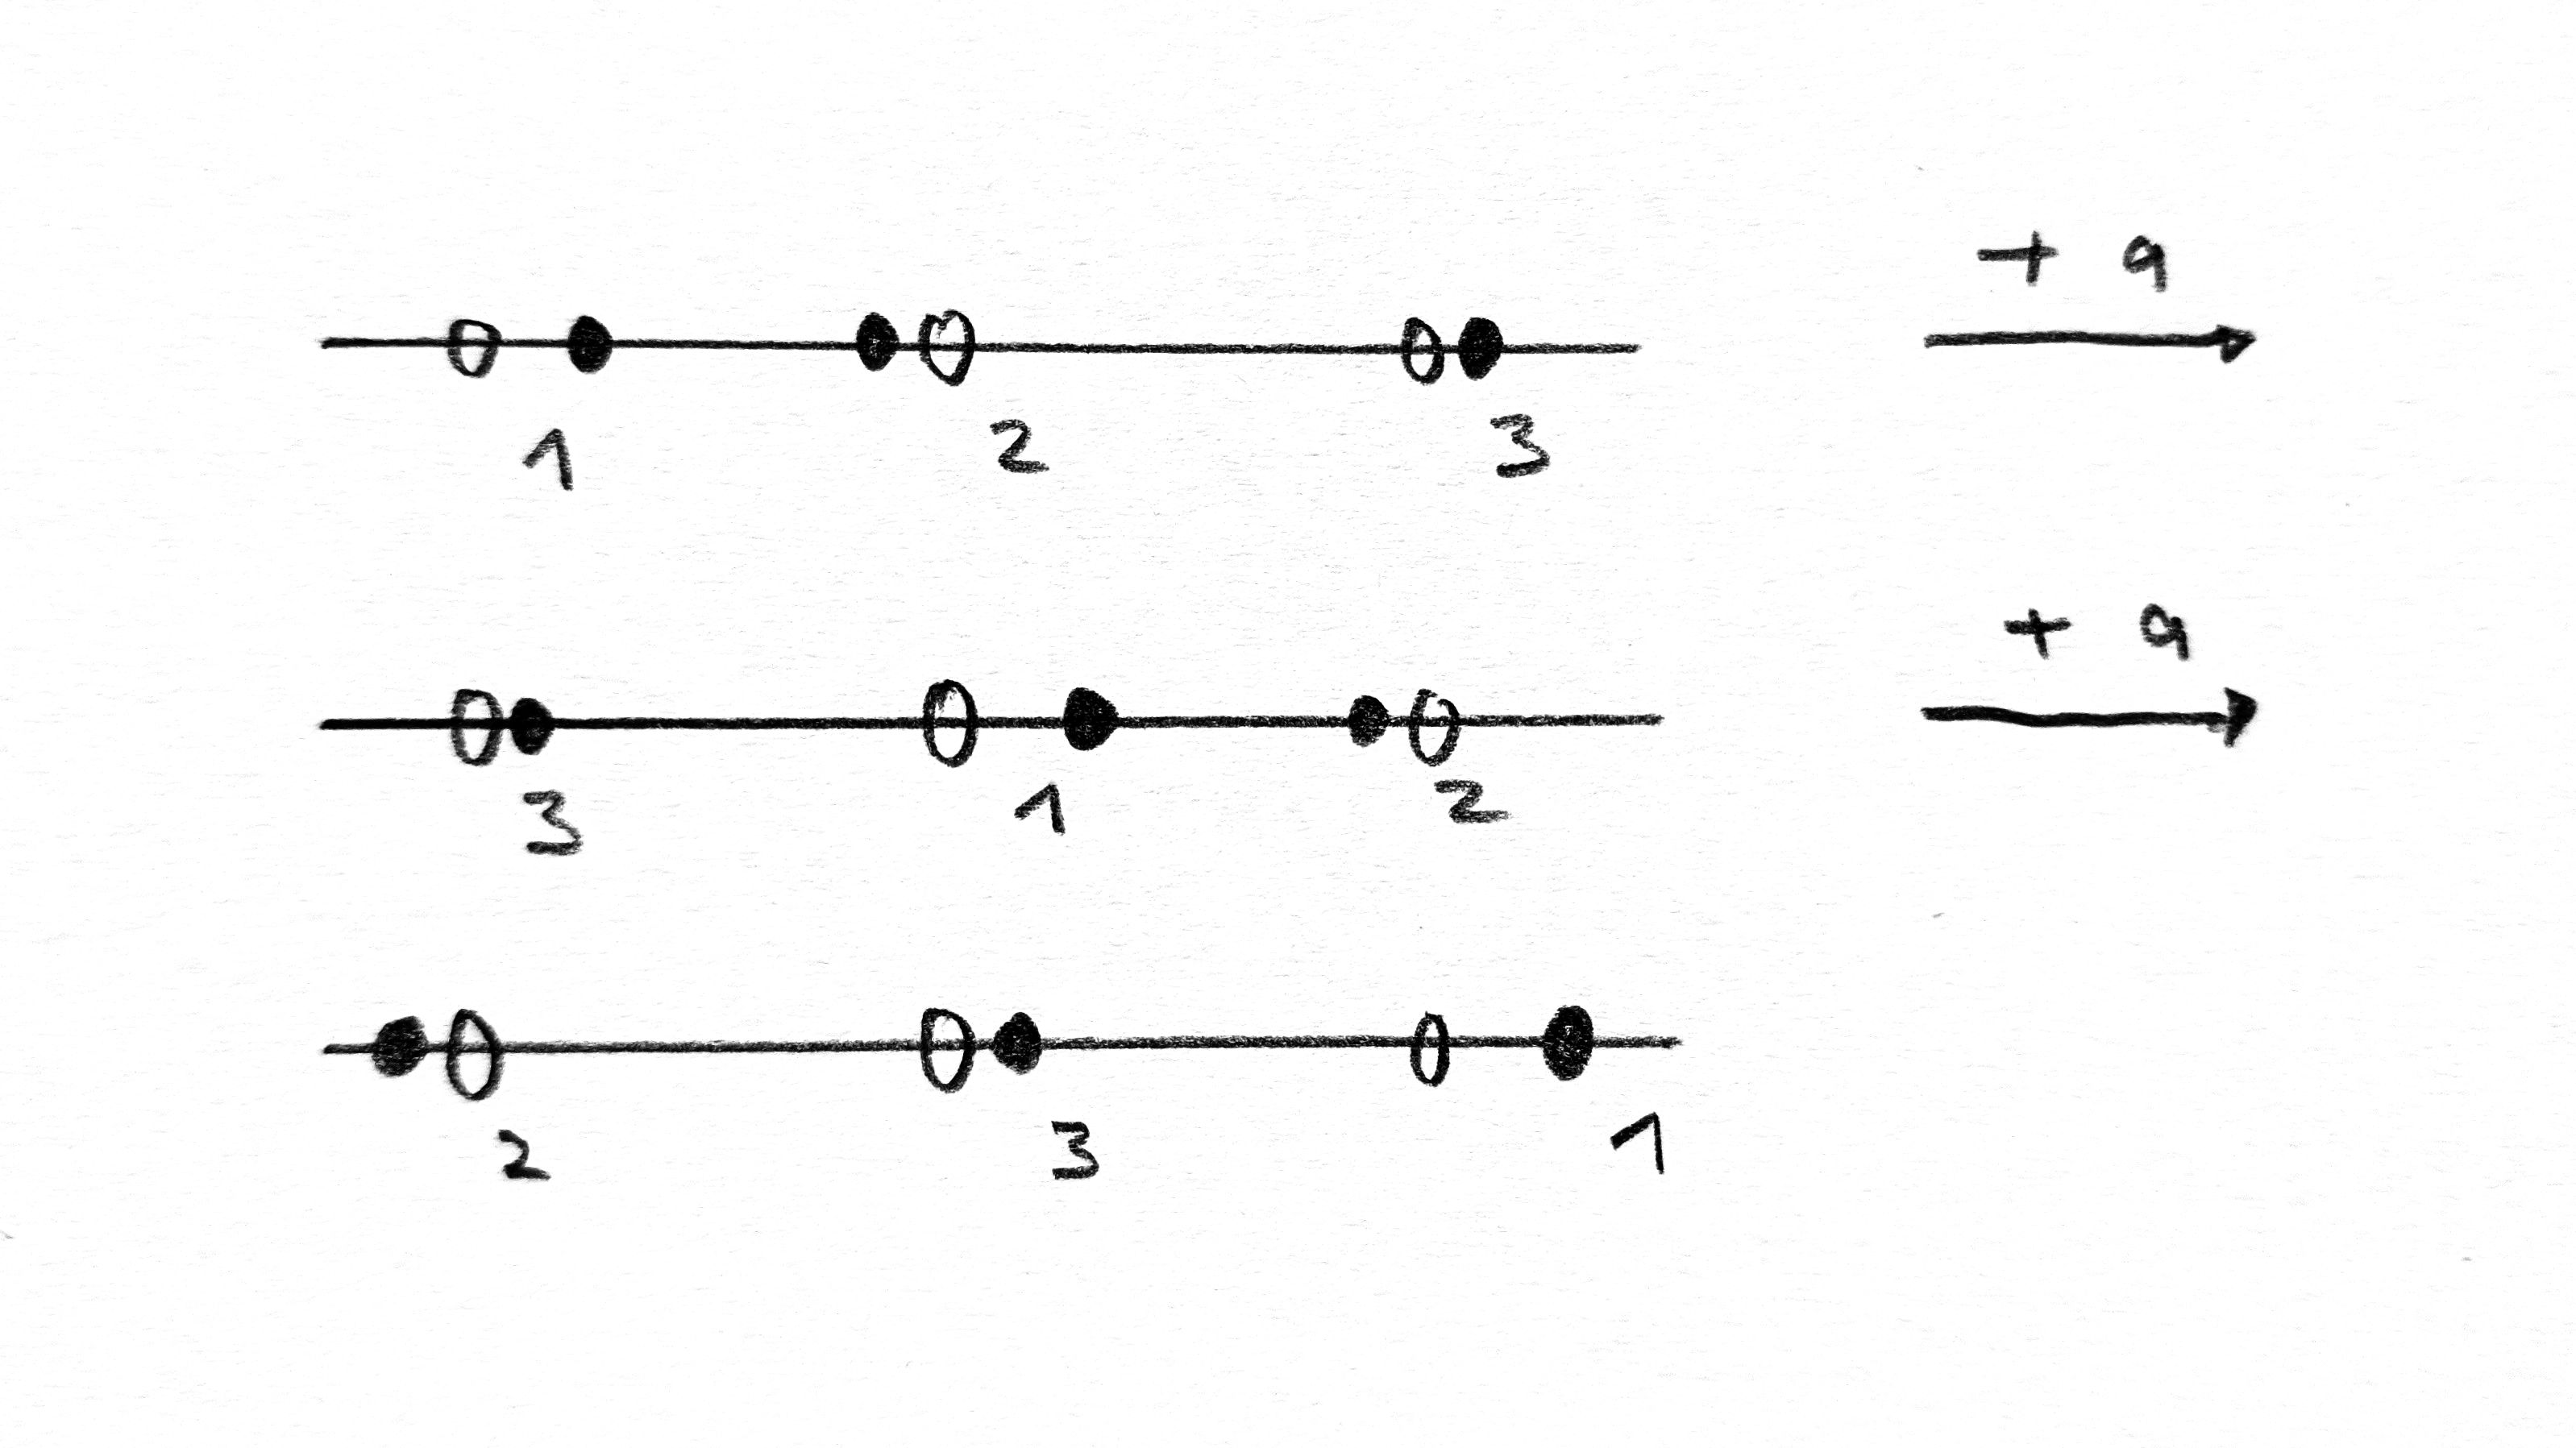
\includegraphics[width=.68\textwidth]{./sketches/permutation1.jpg}
	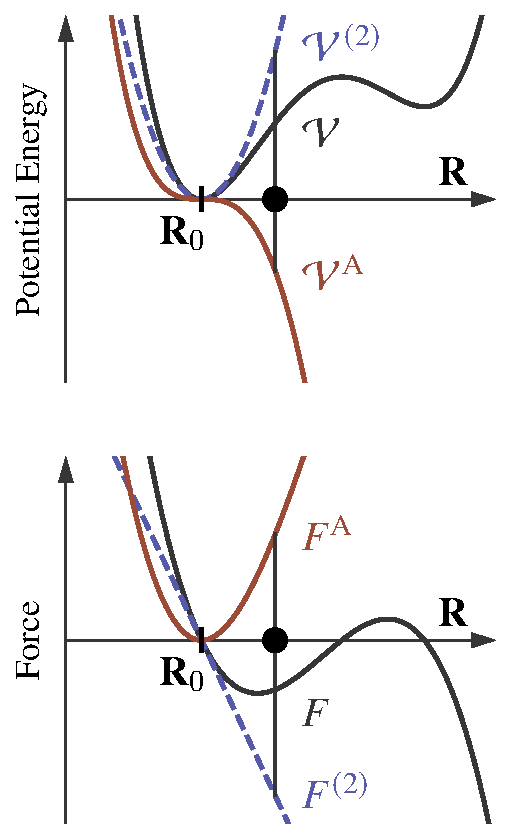
\includegraphics[width=\textwidth]{./data/plots/anharmonicity/1_pes_sketch/sketch_vertical.pdf}
	\caption{Upper: Sketch of a one-dimensional potential-energy surface $\mathcal V$ (solid black), its harmonic approximation $\mathcal{V}^{(2)} (\b R)$ (dashed blue), and the anharmonic contribution $\mathcal{V}^{\rm A} (\b R)$ (solid red). Lower: The force ${F} ({\bf R})$ given by the derivative of $\mathcal V$ (black), the force $F^{(2)}$ stemming from $\mathcal{V}^{(2)} (\b R)$ (blue), and the anharmonic contribution $F^\mathrm{A} = F - F^{(2)}$ (red), cf.~Eq.\,\eqref{eq:anh.F}.}
	\label{fig:pes_sketch_vertical}
\end{marginfigure}

In accordance with the previous chapters, classical nuclear dynamics within the Born-Oppenheimer approximation is governed by the Hamiltonian
\begin{align}
	\mathcal H ( {\bf P}, {\bf R}) 
		= \sum_I \frac{\b P_I^2}{2 M_I} + \mathcal V (\b R)~,
	\label{eq:anh.H}
\end{align}
where $\bf P$ and $\bf R$ denote the atomic momenta and coordinates. Using an expansion of the the full potential $\mathcal V ({\bf R})$ in the displacements $\bf U$ around a reference configuration ${\bf R}^0$ as discussed in Chp.\,\ref{chp:dynamics}, the potential can be split into a harmonic contribution, $\mathcal V^{(2)}$, and a second term capturing all anharmonic effects, $\mathcal V^{\rm A}$,
\begin{align}
	\mathcal V ({\bf R})
		= \mathcal V^{(2)} ({\bf R}) + \mathcal V^{\rm A} ({\bf R})~.
	\label{eq:anh.V}
\end{align}
In the classical limit, the dynamical evolution of the nuclei is determined by the potential through the interatomic forces as defined Eq.\,\eqref{eq:dyn.eom.classical},
\begin{align}
	M_I \ddot{\bf R}_I
		= -\frac{\partial \mathcal V}{\partial {\bf R}_I}
		\equiv {\bf F}_I~,
\end{align}
~i.\,e.,~Newton's equations of motion. By linearity of the differential, the forces can therefore be split into harmonic and anharmonic contributions as well,
\begin{align}
	{\bf F}_I
		= {\bf F}_I^{(2)} + {\bf F}_I^{\rm A}~.
	\label{eq:anh.F}
\end{align}
The division of potential and forces into harmonic and anharmonic contributions is depicted for a one-dimensional potential in Fig.\,\ref{fig:pes_sketch_vertical}.



\section{Anharmonicity measure}
\label{sec:anharmonicity_measure}

\begin{marginfigure}
	\centering
	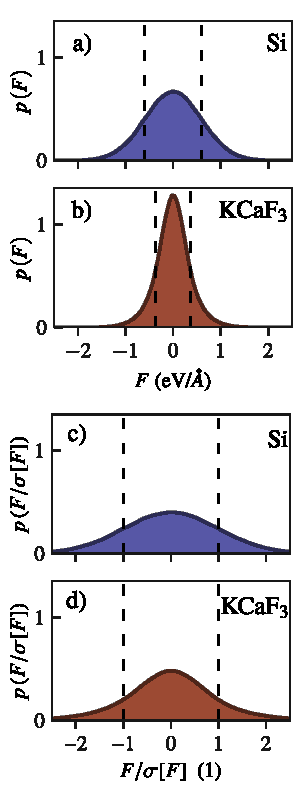
\includegraphics[width=0.8\textwidth]{./data/plots/anharmonicity/4_force_distribution/histogram_forces_vertical.pdf}
	\caption{
		Force component distribution before and after normalization with the width of the distribution $\sigma [F]$. $p(F)$ denotes the probability to find a force component $F_{I, \alpha}$ of strength $F$ in the material. Panel a) and b) show the distribution before normalization, c) and d) after normalization. Dashed vertical lines denotes the standard deviation of the displayed distribution.
	}
	\label{fig:anh.normalization}
\end{marginfigure}

We base the definition of a measure for anharmonicity on the forces, for two reasons: First, because the forces give microscopic insight, as they can be resolved per atom. Second, the forces are statistically easier to describe, since per configuration $\bf R$, there are $3N$ force components ${\bf F} = ({\bf F}_1, \ldots, {\bf F}_N)$.

In terms of the force contributions defined in Eq.\,\eqref{eq:anh.F}, we define a \emph{measure of anharmonicity}, $\sigmaA$, in the following way:
\begin{align}
	\sigmaA (T)
		% = \frac{\sigma [F^{\rm A}]_T}{\sigma [F]_T}
		= \sqrt{\frac{\sum_{I, \alpha} \braket{(F^{\rm A}_{I, \alpha})^2}_T}{\sum_{I, \alpha} \braket{(F_{I, \alpha})^2}_T}}~,
	\label{eq:sigmaA}
\end{align}
where $F_{I, \alpha}^{(A)}$ is the $\alpha$ component of the (anharmonic) force on atom $I$ and $\braket{\cdot}_T$ denotes a thermodynamic average at temperature $T$. The measure $\sigmaA$ quantifies the anharmonic strength in terms of the standard deviation of the distribution of anharmonic force components at a given temperature, $\sigma [F^{\rm A}]_T$, normalized by the standard deviation of the actual force distribution, $\sigma [F]_T$, The standard deviation of a force distribution is defined as
\begin{align}
	\sigma [F]_T 
		= \sqrt{\frac{1}{3N} \sum_{I, \alpha} \braket{F_{I, \alpha}^2}_T}~.
\end{align}
The effect of normalizing the distribution of forces is shown in Fig.\,\ref{fig:anh.normalization} for the two exemplary materials already discussed in the context of phonon dispersions in Sec.\,\ref{sec:ha.dispersions}, silicon, and the orthorombic perovskite KCaF$_3$. Only after normalizing the forces, a meaningful comparison between materials or across temperatures can be achieved.



\newthought{For the two exemplary materials, we show the joint normalized distributions of force and anharmonic force contributions} in Fig.\,\ref{fig:anh.sigmaA}, where the thermodynamic sampling is performed by \emph{ab initio} molecular dynamics simulations at 300\,K.
\begin{figure}
	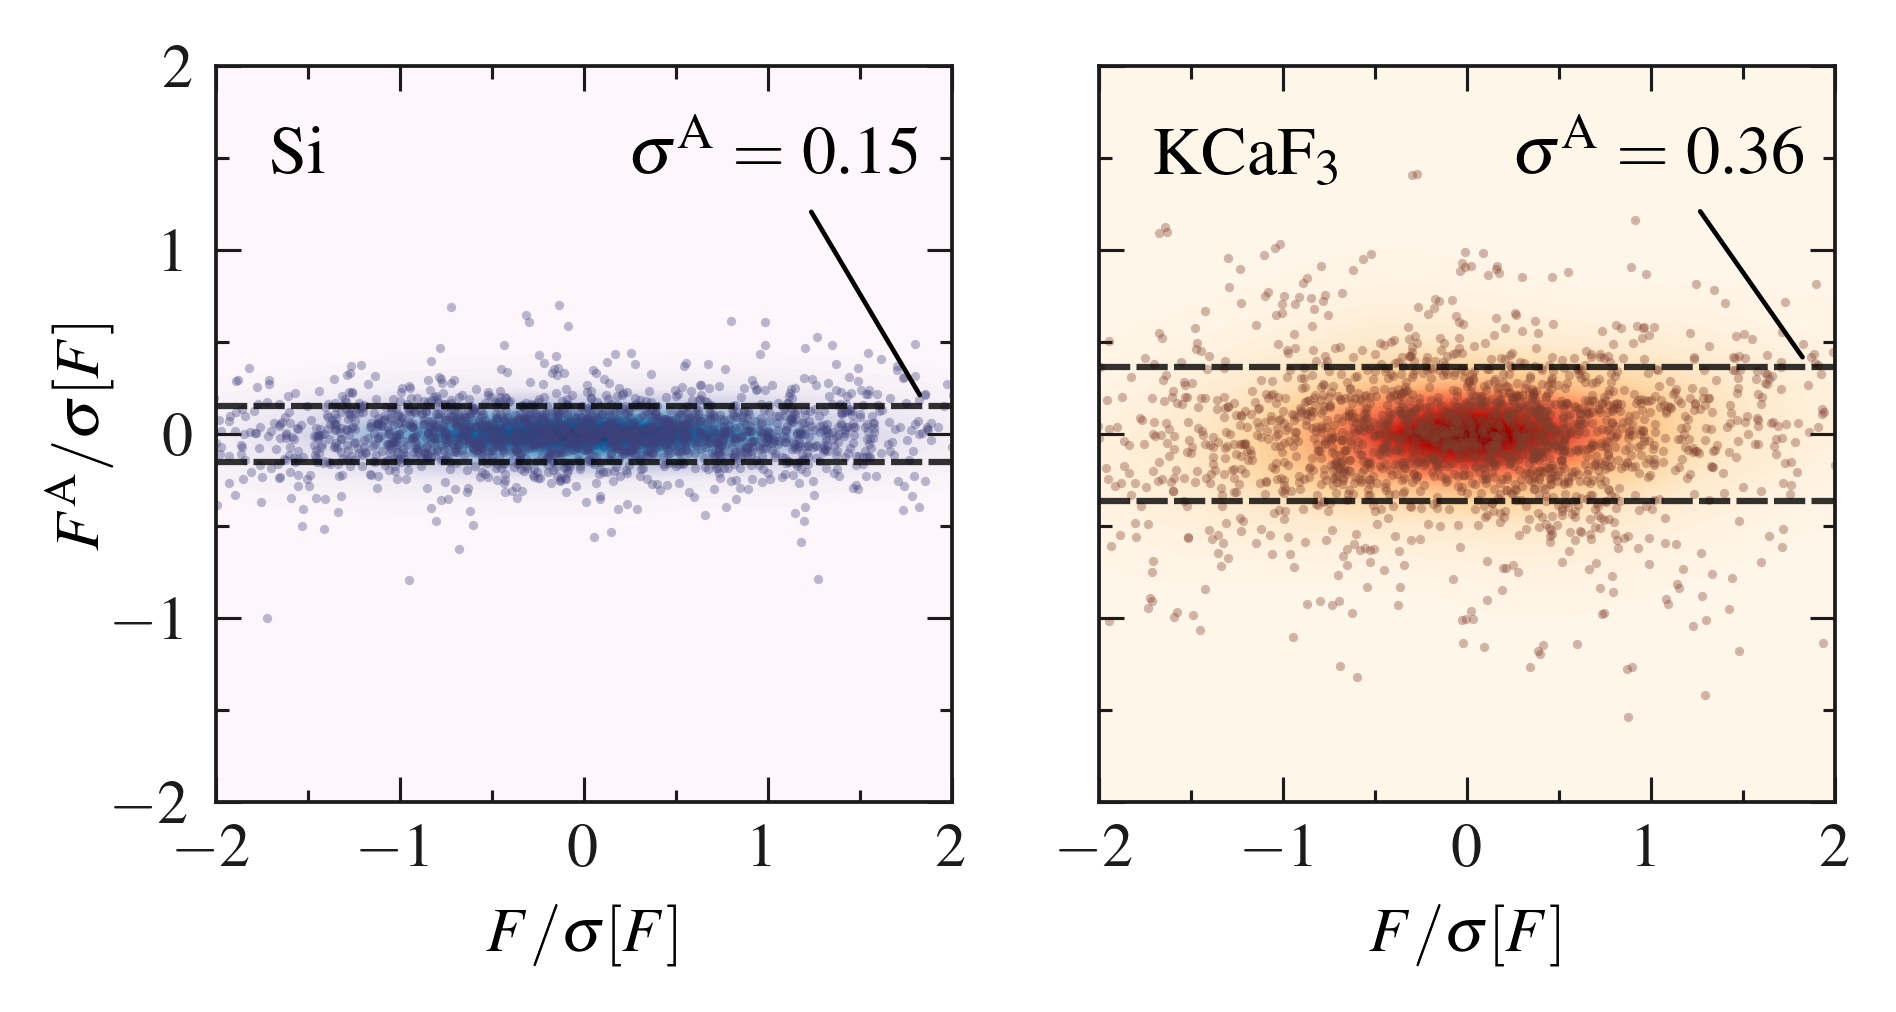
\includegraphics[width=\textwidth]{./data/plots/anharmonicity/5_density_plots/histogram_annotated.png}
	\caption{
		Normalized anharmonic force components versus normalized force components. Dashed horizontal lines: Width of the distribution estimated from standard deviation. Individual dots are force components sampled during an \emph{ab initio} MD simulations.
	}
	\label{fig:anh.sigmaA}
\end{figure}
In this representation, $\sigmaA$ is given by the standard deviation of the distribution in y-direction, as indicated by the dashed horizontal lines in the plot. The distribution of anharmonic force components is more than twice as broad for the perovskite KCaF$_3$ compared to silicon, with a $\sigmaA_{\rm KCaF_3} = 0.36$ compared to $\sigmaA_{\rm Si} = 0.15$. This can be interpreted in the sense that 36\,\% of the forces stem from anharmonic contributions in KCaF$_3$, and 15\,\% in silicon. Furthermore, strongly anharmonic force contributions with a strength of $0.5\,\sigma [F]$ or more are nearly absent in silicon with a probability of $<0.01\,\%$, whereas anharmonic forces of this strength in KCaF$_3$ occur with a much higher probability of $\sim 16.5\,\%$.


\newthought{The anharmonicity measure defined in Eq.\,\eqref{eq:sigmaA}} can also be evaluated for subsets of the dynamical degrees of freedom,~e.\,g.,~per chemical species, as shown in Fig.\,\ref{fig.anh.sigmaA.atoms}.
\begin{figure}
	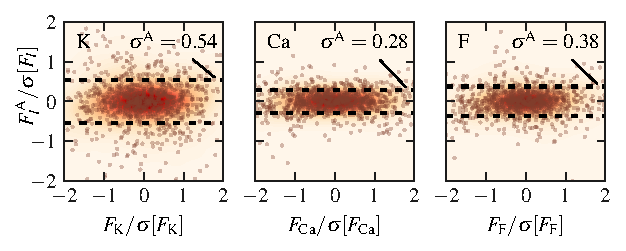
\includegraphics[width=\textwidth]{./data/plots/anharmonicity/5_density_plots/histogram_atoms.pdf}
	\caption{
		Normalized anharmonic force components versus normalized force components. Dashed horizontal lines: Width of the distribution estimated from standard deviation.
	}
	\label{fig.anh.sigmaA.atoms}
\end{figure}
In the example of KCaF$_3$, this analysis shows that the calcium (Ca) atoms occupying the vertices of the unit cell are comparatively well described by the harmonic model, whereas the description of potassium (K) is particularly bad. This can be explained by the phase-transition mechanism observed in KCaF$_3$: Above 560\,K, the material becomes cubic, and the octahedral displacement of fluorine~(F) is removed, as shown in Fig.\,\ref{fig:anh.KCaF3}. This tilt also affects the potassium atoms, which are displaced from their high-temperature reference position in the orthorombic phase, and are therefore located in a shallow potential already at room temperature, well below the phase transition~\cite{Bulou.1980,Hidaka.1984}.
\begin{marginfigure}
	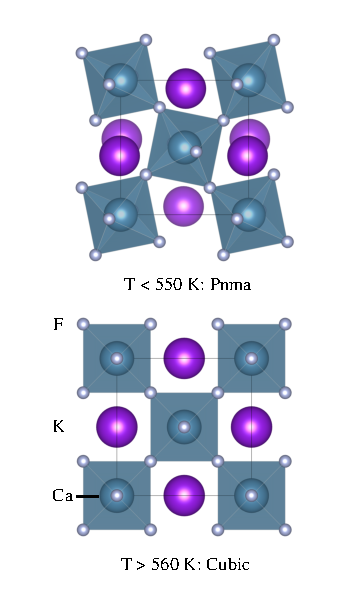
\includegraphics[width=\textwidth]{./data/plots/anharmonicity/2_materials/both.pdf}
	\caption{
		KCaF$_3$ in the low-temperature Pnma~(top) and high-temperature cubic phase~(bottom). Both structures are viewed along the long $b$-axis.
	}
	\label{fig:anh.KCaF3}
\end{marginfigure}

\newthought{It is instructive to evaluate the anharmonicity for single configurations}, be it snapshots in time during molecular dynamics simulations, or when using other sampling approaches,~e.\,g,~harmonic Monte Carlo samples as defined in Eq.\,\eqref{eq:ha.samples}. The sample-resolved anharmonicity is given in analogy to Eq.\,\eqref{eq:sigmaA} as
\begin{align}
	\sigmaA [{\bf R}]
		= \sqrt{\frac{\sum_{I, \alpha} (F^{\rm A}_{I, \alpha})^2}{\sum_{I, \alpha} {(F_{I, \alpha})^2}}}~.
	\label{eq:sigmaA.sample}
\end{align}
While we will discuss ``time-resolved anharmonicity'' in detail at a later point, we show the evaluation of $\sigmaA$ for samples generated by Eq.\,\eqref{eq:ha.samples} in Fig.\,\ref{fig:anh.sampling}.
\begin{figure}
	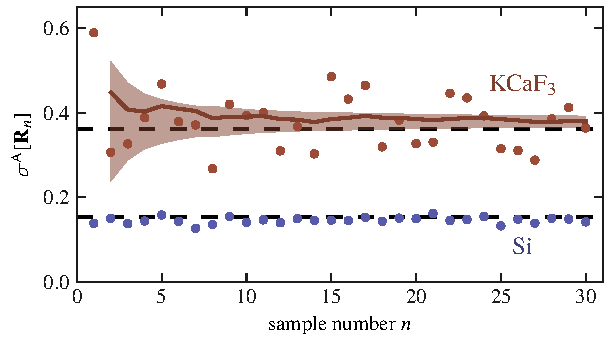
\includegraphics[width=4.1in]{./data/plots/anharmonicity/7_sampling/convergence_sigma_MC.pdf}
	\caption{
			Anharmonicity measure $\sigmaA$ evaluated for individual atomic configurations obtained from Eq.\,\eqref{eq:ha.samples}. Dots: $\sigmaA [{\bf R}_n]$ for individual samples; Red line: Cumulative average.	Black dashed line: $\sigmaA$ from aiMD.	Shadowed region: Convergence estimated by standard error.
	}
	\label{fig:anh.sampling}
\end{figure}
The analysis shows that a decent estimate of $\sigmaA$ can be obtained from the harmonic sampling analysis with few samples. Especially in silicon, each individual harmonic sample yields a $\sigmaA$ within 99\,\% of the reference value obtained by MD simulations for several hundred simulation time steps, which is indicated by the dashed horizontal line. For the more anharmonic KCaF$_3$, the harmonic sampling with 30~samples yields an estimated value of $\sigmaA_{\rm est.} = 0.38$, which differs from the MD value ($\sigmaA = 0.36$) by about 5\,\%. A distinction between largely harmonic materials like silicon, and anharmonic materials like KCaF$_3$, is therefore possible with very few samples.

Motivated by this fact, we investigated the possiblity to estimate $\sigmaA$ based on a single sample, as suggested by Zacharias and Giustino in Ref.\,\cite{Zacharias.2016}: They use a single, deterministic sample to probe the most probable part of the harmonic distribution by choosing $\zeta_s = (-1)^s$ instead of a random distribution in Eq.\,\eqref{eq:ha.samples}. We denote anharmonicity measures obtained by such a ``one-shot'' approach by $\sigmaAOS$ in the following. As shown in Fig.\,\ref{fig:anh.one-shot}, the one-shot samples provide very good estimates for silicon in the the entire temperature range from 200\,K to 800\,K, which can be expected due to the largely harmonic nature of silicon.
\begin{figure}
	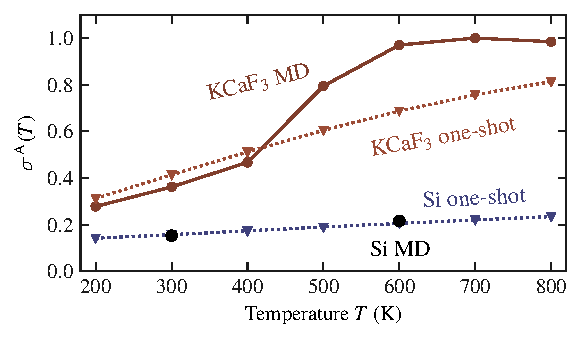
\includegraphics[width=4.1in]{./data/plots/anharmonicity/7_sampling/sigma_temp_one_shot.pdf}
	\caption{
		$\sigmaA$ as a function of temperature obtained from MD~simulations (black circles) and one-shot sampling (triangles connected by dashed curves)
	}
	\label{fig:anh.one-shot}
\end{figure}
For KCaF$_3$, the agreement is decent in the temperature range from 200\, to 400\,K, at least within the limits of the harmonic sampling approach as discussed in the previous paragraph. Above 500\,K, the difference to the reference value from MD simulations increases, which is due to the phase transition mechanism in KCaF$_3$ discussed earlier:
%: This phase transition also occurs in the simulation cell. 
A prediction of anharmonicity across phase transitions cannot be expected from simple harmonic sampling approaches, because the entire reference frame for the harmonic model changes when a phase transition occurs. The phase transition mechanism of KCaF$_3$ and implications for the anharmonicity measure are further discussed in Ref.\,\cite{Knoop.2020}.

\newthought{Ultimately, the applicability of the one-shot sampling approach} needs to be assessed for a diverse set of materials, especially if one aims to use this scheme to screen for anharmonicity in material space. As shown in Fig.\,\ref{fig:anh.screening} for a set of 63~materials, the one-shot sampling is reliable within $\pm 10\,\%$ for all materials in the set, up to a value of about $\sigmaA \simeq 0.2$.
\begin{figure}
	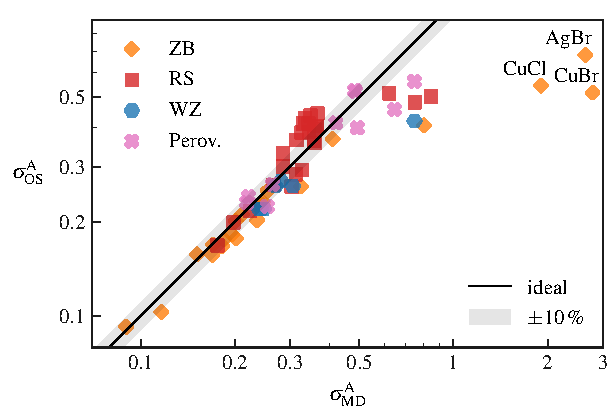
\includegraphics[width=4.1in]{./data/plots/anharmonicity/8_screening/sigma_os_md.pdf}
	\caption{
		Comparison of the anharmonicity measure obtained from MD simulations and one-shot sampling (OS) for 63 materials at 300\,K. The set comprises 25 rock salt (RS), 21 zincblende (ZS), 7 wurtzite (WZ), and 10 orthorombic perovskite (Perov.) materials. The diagonal line denotes perfect agreement between MD and OS, and the green area denotes a 10\,\%~error margin to guide the eye.
		Data was taken from Ref.\,\cite{Knoop.2020}.
	}
	\label{fig:anh.screening}
\end{figure}
For larger values of $\sigmaA$, the deviation can become larger, especially for the group of rock salt materials with $\sigmaA \simeq 0.35$ (red squares) where the one-shot sampling overestimates $\sigmaA$ by about 20\,\%. Nevertheless, the agreement is qualitatively correct up to values of about $\sigmaA \simeq 0.4$, after which materials begin to show effects not captured by the harmonic sampling,~e.\,g.,~phase transitions as discussed earlier for KCaF$_3$. In particular, the three highlighted noble metal halides AgBr, CuCl, and CuBr deviate strongly. These materials tend towards non-perturbative effects during the MD simulation such as spontaneous defect formation~\cite{Knoop.2020}, which is a dynamical effect impossible to describe by any fixed-reference harmonic model. We will discuss the nature of these effects in more detail later in Sec.\,\ref{sec:dynamical_effects}. 

To conclude, we point out that also in the case of non-trivial dynamical effects such as defect formation, the estimated anharmonicity scores $\sigmaAOS$ are larger than $\gtrapprox 0.5$, and therefore indicate strong anharmonicity. A qualitative classification of strong anharmonicity in terms of one-shot sampling is therefore possible for all materials in the set, while quantitative agreement is only achieved for clearly harmonic materials with $\sigmaA \lesssim 0.2$.


\section{Anharmonicity and thermal conductivity}
\label{sec:kappa_vs_sigmaA}

Based on the qualitative discussion of thermal transport in Sec.\,\ref{sec:hf.kappa.ha}, one may expect that stronger anharmonicity leads to shorter phonon lifetimes and therefore lower thermal conductivity. We tested this hypothesis for 47 materials where experimental data was available~\cite{Morelli.2006,Chen.2019}. The results are shown in Fig.\,\ref{fig:anh.kappa}.
%
\begin{figure}
	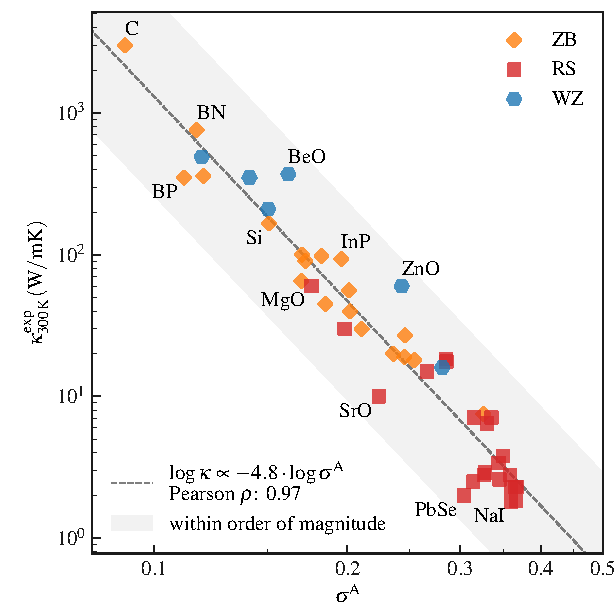
\includegraphics[width=4.1in]{./data/plots/anharmonicity/9_kappa/sigma_vs_kappa.pdf}
	\caption{
		Experimental thermal conductivity at room temperature, $\kappa^{\rm exp}_{300\,{\rm K}}$, versus one-shot measure of anharmonicity, $\sigmaAOS$, and fully anharmonic $\sigmaAMD$ for materials with $\sigmaAOS > 0.2$. 
		The dashed diagonal line indicates a power law fit for the data. The grey area denotes values of $\kappa$ which agree with the fit within 50\,\% to guide the eye. The dataset contains 47 materials, 22 rock salt (RS), 19 zincblende (ZB), and 6 wurtzite (WZ) structures. Experimental data from Ref.~\cite{Morelli.2006,Chen.2019}.
	}
	\label{fig:anh.kappa}
\end{figure}

The analysis reveals an inverse power law relationship between thermal conductivity and anharmonicity for the materials in the dataset,~i.\,e.,~a linear relationship between the logarithms of $\kappa$ and $\sigmaA$, with a Pearson correlation coefficient of 0.97~\cite{Parzen.1960}:
%
\begin{align}
  \kappa (\sigmaA)
    \approx 0.02 \cdot (\sigmaA)^{-4.8}
\end{align}
%
 Given that just a single descriptor is used,~i.\,e.,~the estimated anharmonicity score, and no further vibrational properties as commonly employed in semi-empirical models for thermal condcutivity~\cite{Toberer.2011,Chen.2019}, this correlation is surprisingly good and indicates that $\sigmaA$ captures some essential physics relevant to heat transport: It is known that diamond (C) is extremely harmonic, so that its thermal conductivity is exceptionally high~\cite{Haas.1938,Klemens.1958}. This is confirmed here with diamond being the most harmonic material studied, with $\sigmaA_{\rm C} = 0.09$ and $\kappa_{\rm C} = 3000$\,W/mK~\cite{Morelli.2006}. On average, the zinc blende (ZB) compounds are more harmonic then the rocksalt (RS) compounds in this dataset, and likewise show higher thermal conductivities. This relation can be explained by the stronger covalent bonding character and higher coordination number in the tetrahedrally coordinated zinc blende compounds, compared to the more ionic, octahedrally coordinated rocksalt materials~\cite{Miller.2017}, which explains the clustering of rocksalt materials in the lower right part of Fig.\,\ref{fig:anh.kappa}.
 
 A notable exception in the class of rocksalt materials is the largely harmonic magnesium oxide (MgO), with $\sigmaA_{\rm MgO} = 0.18$ and $\kappa_{\rm MgO} = 60$\,W/mK~\cite{Morelli.2006}.

%\mscomment{Why are the rock salts bottom right?}
%\FK{More ionic character and therefore weaker bonding on average compared to ZB and WZ.}
%\mscomment{tell that these are ``close to harmonic materials''}
%\FK{not sure they are}
%\mscorrect{why Pearson rho? What does it tell?}
%\mscorrect{why is an order of magnitude ok here?}
%\mscorrect{it looks more than an order of magnitude}


\newthought{The most important messages from Fig.\,\ref{fig:anh.kappa} can be summarized as follows}, adopting the definition suggested by Morelli and Slack to define ``high thermal conductivity'' as $\kappa \gtrsim 50 \, {\rm W/mK}$~\cite{Morelli.2006}:
\begin{enumerate}
	\item Very harmonic materials with $\sigmaA \simeq 0.1$, like diamond ($\sigmaA_{\rm C} = 0.09$), boron phosphide ($\sigmaA_{\rm BP} = 0.11$), or boron nitride ($\sigmaA_{\rm BN} = 0.12$) can be expected to be very good thermal conductors with $\kappa \gtrsim 100\,{\rm W/mK}$.
	\item Strongly anharmonic materials with $\sigmaA \gtrsim 0.3$ can be expected to be poor thermal conductors with $\kappa \lesssim 10\,{\rm W/mK}$.
%    \mscomment{would you say 0.3 still works with BTE?}
%    \FK{yes, with more sophisticated approaches than 0K third order, see discussion in \cite{Ravichandran.2018} for NaCl.}
% discussed later
	\item $\sigmaA$ has a strong correlation with thermal conductivity across the entire dataset, but nevertheless only a rough estimate can be made solely based on $\sigmaA$, especially in the middle region with $\sigmaA \simeq 0.2$. This can be seen by comparing strontium oxide (SrO) with $\kappa = 10\,{\rm W/mK}$ and $\sigmaA = 0.22$, and zinc oxide (ZnO) with $\kappa = 60\,{\rm W/mK}$ and $\sigmaA = 0.24$, or beryllium oxide (BeO) with $\kappa = 370\,{\rm W/mK}$ and $\sigmaA = 0.16$ to magnesium oxide (MgO) with $\kappa = 60\,{\rm W/mK}$ and $\sigmaA = 0.18$. These pairs of materials differ only slightly in their estimated anharmonicity, but still quite strongly in the thermal conductivity, clear evidence for the fact that other material properties determine thermal transport. 
% Nevertheless, the correct order of magnitude of $\kappa$ as indicated by the grey area in Fig.\,\ref{fig:anh.kappa} can always be predicted for the investigated materials.
\end{enumerate}

{These findings suggest the following approach} towards screening material space in search for thermal insulators with $\kappa < 10\,{\rm W/mK}$: Estimate the anharmonicity for materials of interest and focus on the anharmonic ones with $\sigmaA > 0.2$, as more harmonic materials will very likely have higher thermal conductivies.
%\mscomment{sounds bad. Are there examples for thermal insulators with $\sigmaA < 02$}
%\FK{not in our data.}
%\ADD{worst example}
%\mscomment{more importantly: can we use BTE yes/no? important for material space exploration}

Of course, the reverse approach could be pursued when searching for materials with potentially high thermal conductivity.

\section{Candidate materials}
\begin{marginfigure}
	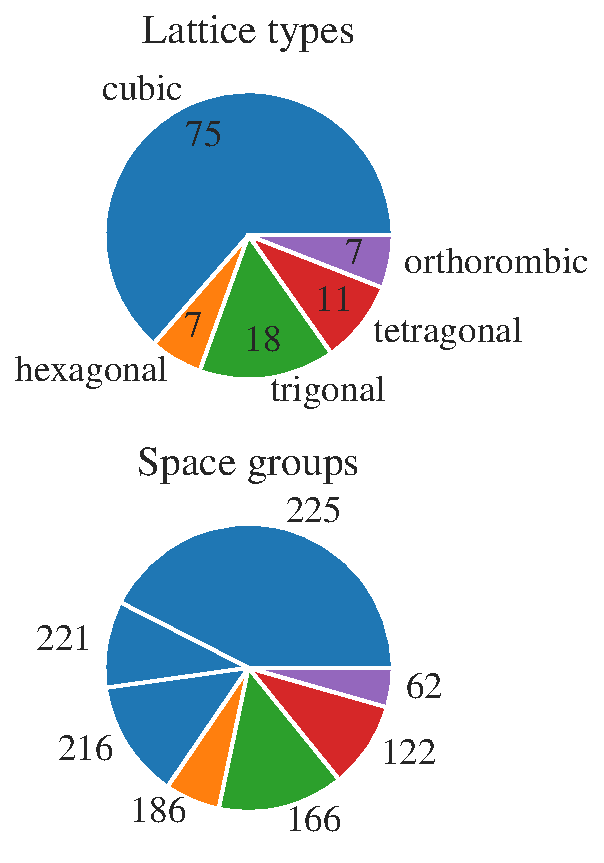
\includegraphics[width=\textwidth]{./data/plots/dataset/pies.pdf}
	\caption{
		Lattice types and space groups represented in the dataset. Space groups not shown in the pie chart: 56, 61, 160, 164, 206, with one representative each.
	}
	\label{fig:anh.pie}
\end{marginfigure}
Using the measure $\sigmaA$, we have identified a set of 118 binary and ternary materials for further investigation.  % with the \emph{ab initio} Green Kubo (aiGK) approach. 
The materials comprise five lattice types and 12 space groups as summarized in Fig.\,\ref{fig:anh.pie}.
%\begin{figure}
%	\includegraphics[width=\textwidth]{./data/plots/dataset/pies_horizontal.pdf}
%	\caption{
%		Lattice types and space groups represented in the dataset. Space groups not shown in the pie chart: 56, 61, 160, 164, 206, with one representative material each.
%	}
%	\label{fig:anh.pie}
%\end{figure}
Since we are mainly interested in thermal insulators as candidate thermoelectric and thermal barrier coating materials, we focus on anharmonic strengths $\sigmaA > 0.2$ as explained above, with a mean of $\sigmaA=0.31$ and a median of $\sigmaA = 0.29$. Some more harmonic materials like MgO ($\sigmaA = 0.18$) have been included for benchmark purposes. A histogram displaying the distribution of $\sigmaA$ values is shown in Fig.\,\ref{fig:anh.histogram}.
\begin{figure}
	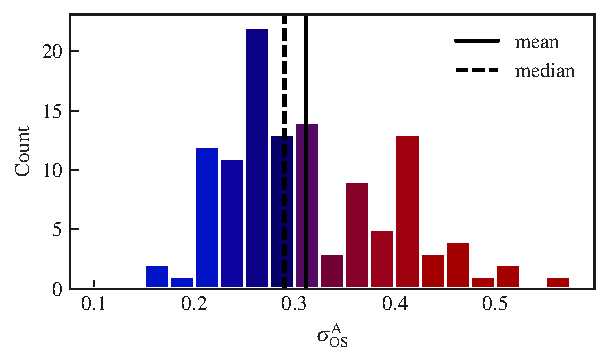
\includegraphics[width=4.1in]{./data/plots/dataset/histogram.pdf}
	\caption{
		Histogram of $\sigmaAOS$ values samples for the 118 chosen materials
	}
	\label{fig:anh.histogram}
\end{figure}
All values are given with respect to room temperature, as this is the regime where the most experimental reference is available to benchmark the aiGK method later on. In total, there are experimental reference values for 45 materials available. These references are given in Tab.\,\ref{tab:kappa.exp} in appendix~\ref{sec:app.experiments}.

% \TODO{Include full list of materials with reference in appendix}

The materials have been chosen based on the following criteria:
\begin{enumerate}
	\item Material has to have an experimentally known stable phase at room temperature,
	\item material has to be semiconductor or insulator with a bandgap large enough to prevent accidental gap closing during molecular dynamics simulations,
	% \mscorrect{it was not explained what happens in this case}
	\item the most heavy element considered is Barium ($Z=56$), after which relativistic effects beyond the ``zeroth order regular approximation'' cannot be neglected~\cite{Vanlenthe.1994,Huhn.2017,Zhao.2021}.
    % \mscorrect{ZORA is not explained anywhere}
\end{enumerate}

%\mscorrect{not just application driven, also Q whether BTE works and when it doesn't there is interesting physics}


%\REM{
%The materials come from these sources:
%From Ramprasad: 41
%From Toberer: 3
%From Springer: 4
%From Roekeghem: 9
%From ICSD: 55
%From Seko: 2
%From AAPL: 4
%}

\newpage

\section{Dynamical effects}
\label{sec:dynamical_effects}
As briefly discussed in Sec.\,\ref{sec:anharmonicity_measure},
%shown in the initial screening of material space presented in Ref.\,\cite{Knoop.2020},
%\mscorrect{this is also part of the thesis, don't just cite}
 strongly anharmonic materials with $\sigmaA > 0.3$ are prone to exhibiting non-trivial dynamical effects such as metastable defect formation and precursors of structural phase transitions. 

\newthought{We carried out \emph{ab initio} molecular dynamics simulations}~\footnote{Computational settings: PBEsol function and \emph{light default} basissets. Time step 4-5\,fs such that the fastest motion corresponding to the highest harmonic vibrational frequency is sufficiently sampled, total simulation time at least 30\,ps. Lattice expansion accounted for by minimizing the pressure in the simulation cell according to the scheme outlined in Sec.\,\ref{sec:app.lattice_expansion}. Full details given in appendix \ref{sec:app.computational_details}.} for each of the candidate materials introduced in the previous chapter to see whether the materials exhibit such non-trivial dynamical effects. 
These dynamical effects can be detected by using a time-resolved anharmonicity measure as defined in Eq.\,\eqref{eq:sigmaA.sample},~i.\,e.,~by evaluating the anharmonicity measure for each sample during the MD with $\sigmaA(t) = \sigmaA [{\bf R} (t)]$, and evaluating fluctuations of $\sigmaA (t)$ in terms of its standard deviation ${\rm std} [ \sigmaA ]$ evaluated along a given trajectory. A comparison of $\sigmaA$ values obtained by one-shot sampling, $\sigmaAOS$, and molecular dynamics, $\sigmaAMD$, is shown in Fig.\,\ref{fig:sigma_os_md_dataset}. Materials with a standard deviation larger than ${\rm std} [ \sigmaAMD ] > 0.01$ are highlighted and labeled.
\begin{figure}
	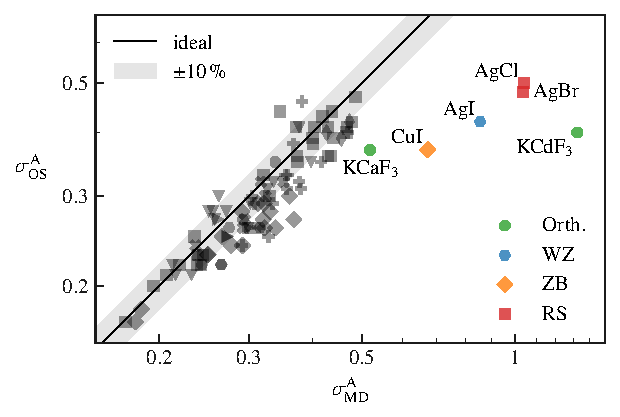
\includegraphics[width=4.1in]{./data/plots/sigma_vs_sigma/sigma_os_md.pdf}
	\caption{$\sigmaA$ values obtained by one-shot sampling (OS) and molecular dynamics simulations (MD) in comparison. Materials with significant fluctuations of the time-resolved anharmonicity measure $\sigmaA (t)$ are highlighted and labeled.}
	\label{fig:sigma_os_md_dataset}
\end{figure}
We discuss the nature of these effects for KCaF$_3$, CuI, AgI, and AgCl in the following. AgBr and KCdF$_3$ are omitted because they behave qualitatively similar to AgCl and KCaF$_3$, respectively. 

The discussion is meant to highlight the prevalence of non-trivial dynamical effects that violate one basic assumption of phonon theory,~i.\,e.,~the assumption of well-defined and stationary reference positions for all atoms in a given phase. Another key insight is that the observed effects are precursors of phase transitions known to occur in these materials at higher temperatures, which means that their onset is observed on the microscopic scale during the dynamic evolution already several 100\,K below the phase transition temperature.
From a methodological point of view, we show how the time-resolved anharmonicity can be used to uncover and explain the nature of the underlying dynamical effect.

%  \mscorrect{honest discussion of simulation times}
%  \FK{this is done for GK, for these static properties 30ps is \emph{grotesquely} overconverged.}
%  \mscorrect{supercell sizes}
%  \FK{beyond the scope of this work, see \cite{Carbogno.2016} for supercell scaling behavior of interpolation scheme}
%  \mscorrect{I would conclude that above $\sigmaA > .2$ non-perturbative calculation should be performed}
%  \FK{I wouldn't.}



\subsection{KCaF$_3$}
KCaF$_3$ is the perovskite material already discussed in some detail in Sec.\,\ref{sec:anharmonicity_measure}, where the octahedral tilting mechanism typical for this class of materials, and the phase transition phenomenology were presented~\cite{Bulou.1980,Hidaka.1984,Knight.2005}. In total, we performed five $NVE$ simulations for KCaF$_3$, with a simulation time of 30\,ps each. The time resolved anharmonicity measure is displayed for each of those trajectories in Fig.\,\ref{fig:defects.KCaF3.sigmaA}.
We find that in three of the five trajectories, $\sigmaA (t)$ jumps between the reference value of $\sigmaA \approx 0.4$,\footnote{We round to 1 decimal point in the following, which is completely sufficient for the discussion of intermittent jumps.} and increased values between $\sigmaA \approx 0.8$ and $\sigmaA \approx 1.2$.
%
\begin{figure}
	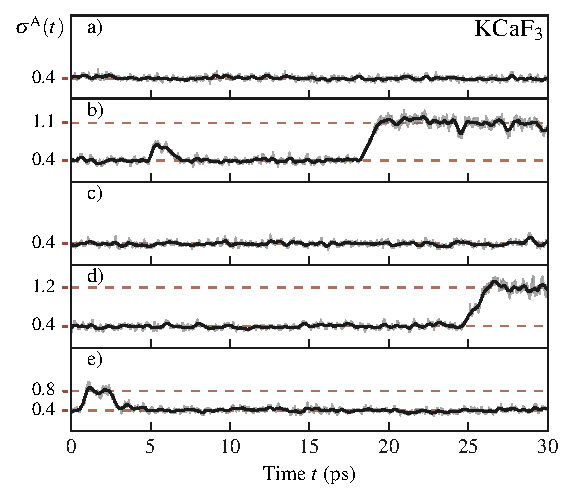
\includegraphics[width=\textwidth]{./data/plots/defects/062.05.KCaF3/sigma_vs_time.pdf}
	\caption{Time-resolved anharmonicity measure $\sigmaA (t)$ for orthorombic KCaF$_3$ in five molecular dynamics runs of 30\,ps length. Increased values of $\sigmaA (t)$ are found in three trajectories (b, d, e).}
	\label{fig:defects.KCaF3.sigmaA}
\end{figure}
%
\newthought{The nature of the underlying dynamical effects} can be resolved by time-averaging the positions ${\bf R} (t)$,
\begin{align}
	{\bf R}_{\rm avg} = \braket{{\bf R} (t)}_t~,	
	\label{eq:R(t).avg}
\end{align}
%
\begin{marginfigure}[-3cm]
	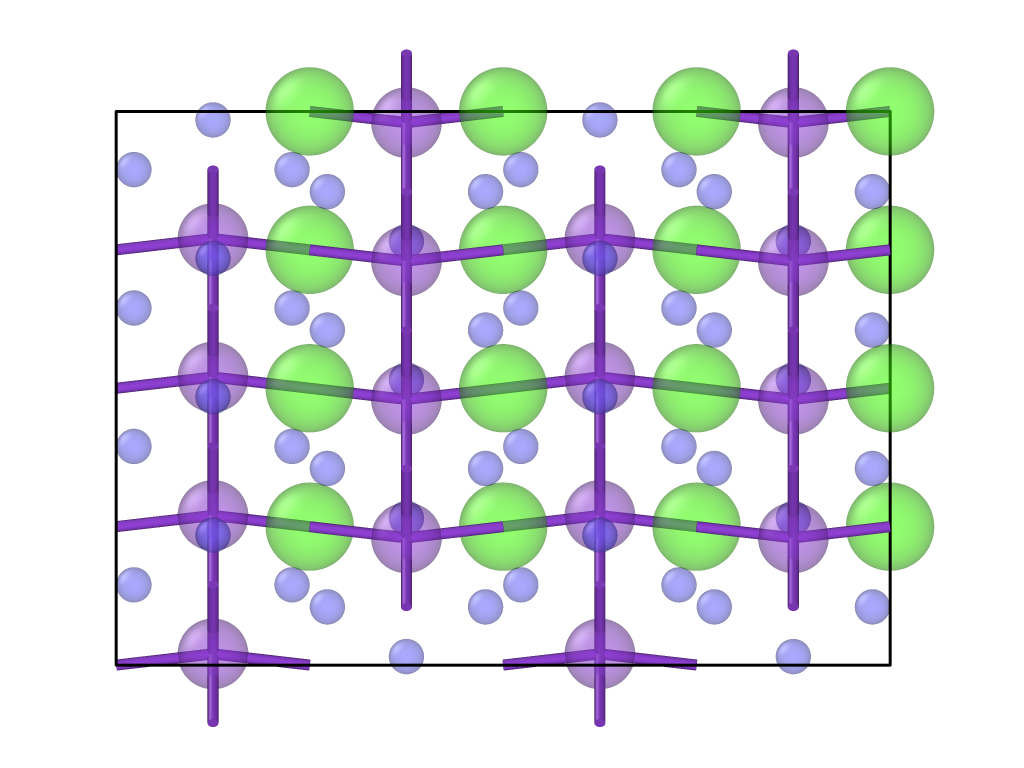
\includegraphics[width=\textwidth]{./data/plots/defects/062.05.KCaF3/plots/ref_left.png}
	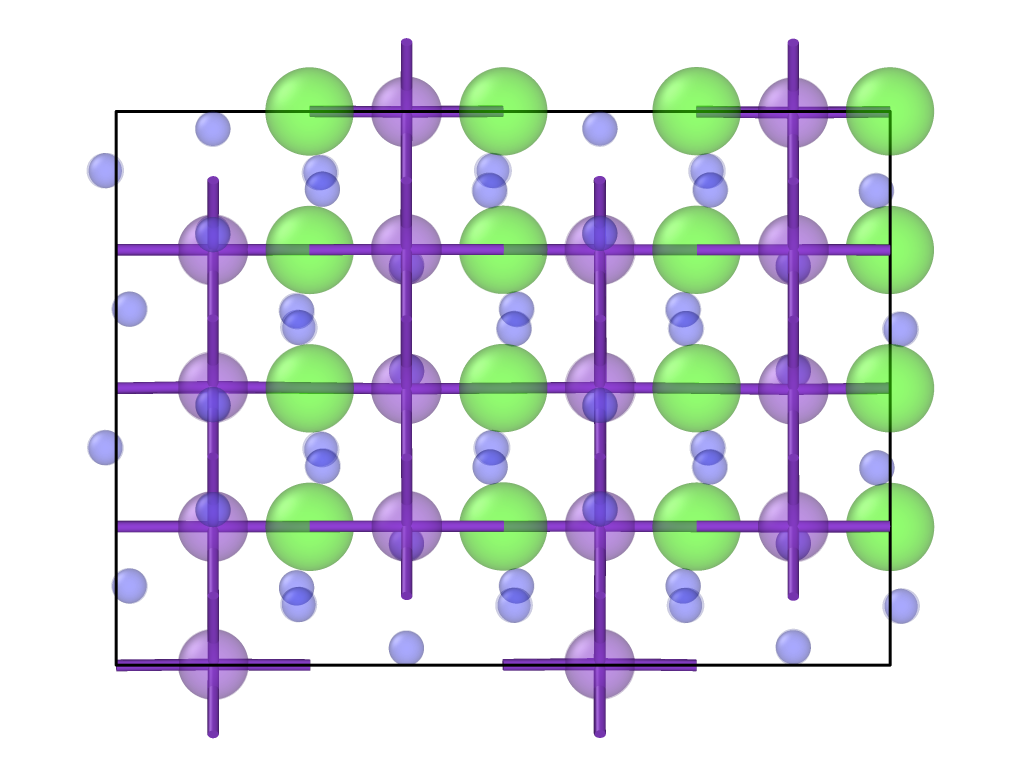
\includegraphics[width=\textwidth]{./data/plots/defects/062.05.KCaF3/plots/2_left.png}
	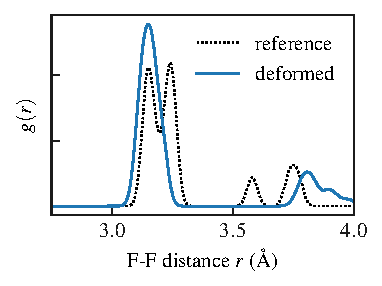
\includegraphics[width=\textwidth]{./data/plots/defects/062.05.KCaF3/rdf/geometry_in_def_2.pdf}
	\caption{Precursor of phase transition in KCaF$_3$. Upper panel: The reference orthorombic structure viewed in (010) direction. The orthorombic displacement of the potassium sub-lattice (violet balls connected by sticks) is clearly visible. Middle panel: When $\sigmaA (t) \approx 1.1$, the potassium sub-lattice temporarily adopts a tetragonal shape. Also the fluorite atoms (small blue balls) reduce their tilt consequently. Lower panel: Radial distribution function $g(r)$ for the fluorine atoms in the orthorombic reference and deformed structure: The number of distinct peaks reduces, reflecting an increase in symmetry when the orthorombic tilt reduces.}
	\label{fig:defects.KCaF3.1}
\end{marginfigure}
\noindent
for the time spans in which $\sigmaA (t)$ is increased. Performing this time average for time spans where $\sigmaA (t) < 0.5$,~i.\,e.,~in situations in which no increase is seen, one recovers the initial orthorombic structure shown in Fig.\,\ref{fig:defects.KCaF3.1} (top figure). When averaging trajectory b) for the time where $\sigmaA (t) \approx 1.1$, the resulting structure is more symmetric, with an approximately tetragonal arrangement of atoms. This can be seen by focusing on the potassium sub lattice (purple atoms connected by sticks) in Fig.\,\ref{fig:defects.KCaF3.1} (middle). The increased symmetry is further revealed by noting that the fluorine cage becomes more ordered, as shown in terms of the F-F pair distribution function in Fig.\,\ref{fig:defects.KCaF3.1} (bottom). This phenomenon can be viewed as a precursor of the phase transitions towards tetragonal and cubic phases known to occur in this material at temperatures higher than 560\,K~\cite{Bulou.1980,Hidaka.1984,Knoop.2020}. However, at 300\,K, well below the transition temperature, this configuration only occurs sporadically on the time scale of several picoseconds during the simulation, and is therefore not fully stabilized.

%\mscorrect{it is not expected that the full supercell adopts the structure but only one/few atoms}
%\FK{Fig. \ref{fig:defects.KCaF3.1} clearly shows that we observe a collective effect and not single atom defects.}

% \newpage

\subsection{CuI}
\label{sec:defects.CuI}

\begin{figure}
	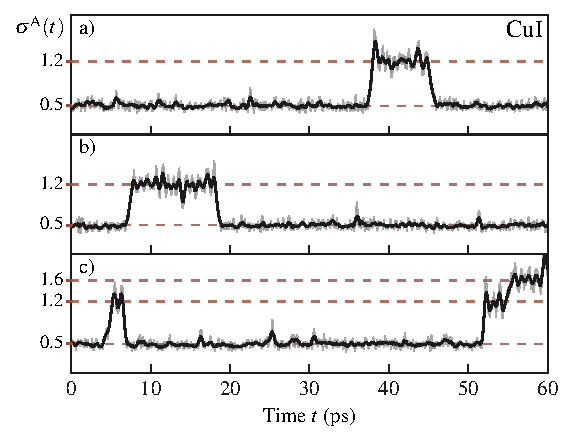
\includegraphics[width=\textwidth]{./data/plots/defects/216.02.CuI/sigma_vs_time.pdf}
	\caption{Time-resolved anharmonicity measure $\sigmaA (t)$ for zincblende CuI in three molecular dynamics runs of 60\,ps length. Increased values of $\sigmaA (t)$ are found in all three trajectories.}
	\label{fig:defects.CuI}
\end{figure}
%
%\mscomment{why don't you show pair distribution function for the time snapshots}
%\FK{I tried by it's difficult to normalize because only 1 of 216 atoms moves. It would be an interesting project to do proper coarse graining on this.}
%
Copper iodide (CuI), also known as marshite, is a simple material with fcc lattice of the zincblende type. This phase is also known as the $\gamma$ phase ($\gamma$-CuI).
The time-resolved anharmonicity measures are shown in Fig.\,\ref{fig:defects.CuI} for three trajectories of 60\,ps simulation time.
The characteristic features are the jumps in $\sigmaA (t)$ from values of $\sigmaA (t) \approx 0.5$ to $\sigmaA (t) \approx 1.2$ or 1.6. In the simulated time period, these values are taken for 3 to 12\,ps, before the initial value of $\sigmaA (t) \approx 0.5$ is restored. 
% The jumps in $\sigmaA (t)$ hint at a dynamical effect which strongly violates the harmonic approximation.
%
\begin{marginfigure}
	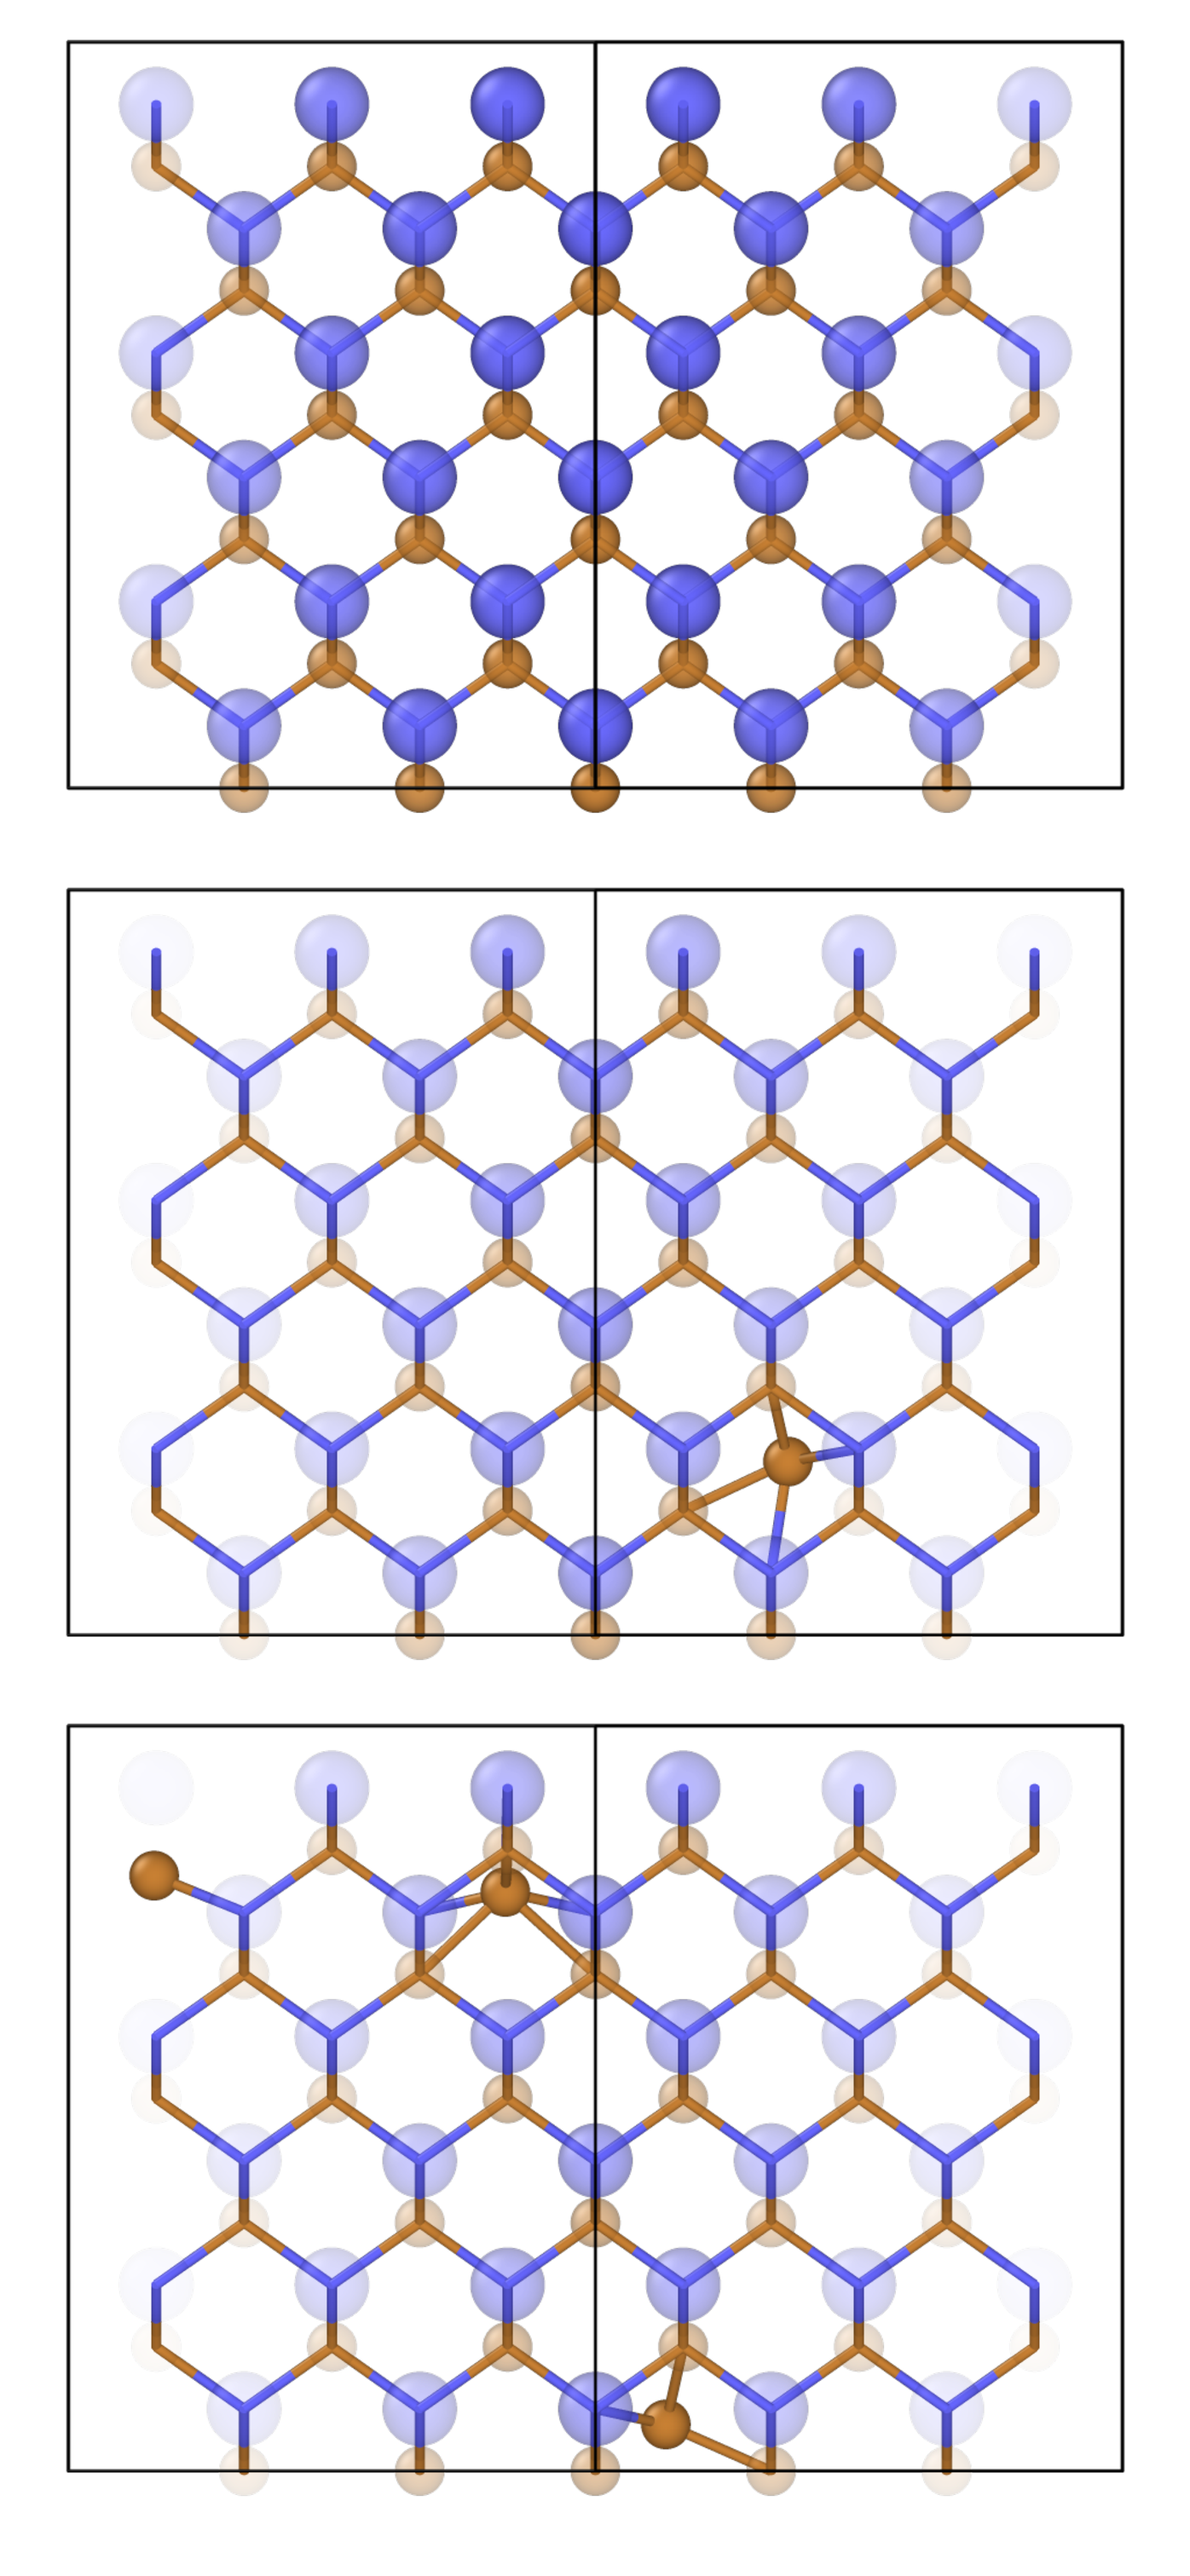
\includegraphics[width=\textwidth]{./data/plots/defects/216.02.CuI/all.pdf}
	\caption{CuI viewed in (110) direction. Top: High-symmetry zincblende structure. Middle: Copper ion in lower-right quadrant moves into interstitial site along (111) direction when $\sigmaA (t) \approx 1.2$. Bottom: Several defects form when $\sigmaA (t) \approx 1.6$}
	\label{fig:defects.CuI.1}
\end{marginfigure} 
%
As in the case of KCaF$_3$, we compare two time-averaged structures in Fig.\,\ref{fig:defects.CuI.1}: A time average with respect to the entire simulation time reveals the perfect zincblende structure of CuI which corresponds to the minimum of the potential-energy surface.
When averaging over the time span where $\sigmaA (t) \approx 1.2$, however, the average structure has one Cu atom diplaced along the (111) direction. Viewing the supercell in (110) direction, the diplacement is clearly visible (Fig.\,\ref{fig:defects.CuI.1}, middle). This means that the Cu occupies a metastable interstitial site at the given position for the respective time period. When $\sigmaA (t)$ is restored to the base value of $\sigmaA (t) \approx 0.5$, the Cu atom moves back to the high-symmetry reference position within the zincblende structure. 
The third trajectory shown in Fig.\,\ref{fig:defects.CuI}~c) evolves to a situation where $\sigmaA \approx 1.6$. This corresponds to a situation, where more than one defects forms~(Fig.\,\ref{fig:defects.CuI.1}, bottom).

\newthought{$\gamma$-CuI is known to undergo a phase transition to a superionic conducting $\beta$ phase} above 643\,K~\cite{Boyce.1979, Boyce.1980,Boyce.1981,Keen.1995}. It is very likely that the defect formation observed in the aiMD simulations at 300\,K are precursors of this phase transition, but too infrequent at this temperature to destabilize the fcc lattice of the $\gamma$ phase.
%\mscorrect{also the other embryos don't destabilize the stable phase}
%\FK{I don't understand, sorry.}

\subsection{AgI}
Wurtzite silver iodide ($\beta$-AgI), or iodargyrite, is another transition metal halide that shares some similarities with $\beta$-CuI discussed in the previous section~\cite{Boyce.1981}. It is known to transition into the superionic conducting $\alpha$ phase above $\sim 420$\,K~\cite{Hoshino.1957,Boyce.1981,Brenner.2020}, and was in fact one of the earliest studied materials exhibiting this phenomenon~\cite{Strock.1934,Strock.1935,Strock.1936}.
%
\begin{figure}
	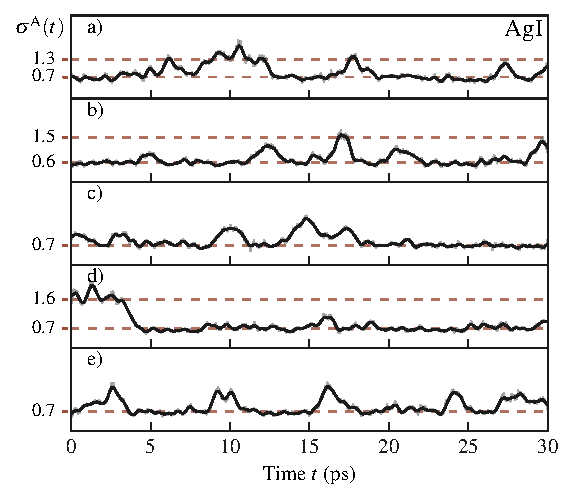
\includegraphics[width=\textwidth]{./data/plots/defects/186.02.AgI/sigma_vs_time.pdf}
	\caption{Time-resolved anharmonicity measure $\sigmaA (t)$ for wurtzite AgI in five molecular dynamics runs of 30\,ps length. Increased values of $\sigmaA (t)$ are found in all five trajectories.}
	\label{fig:defects.AgI}
\end{figure}
%
\begin{marginfigure}
	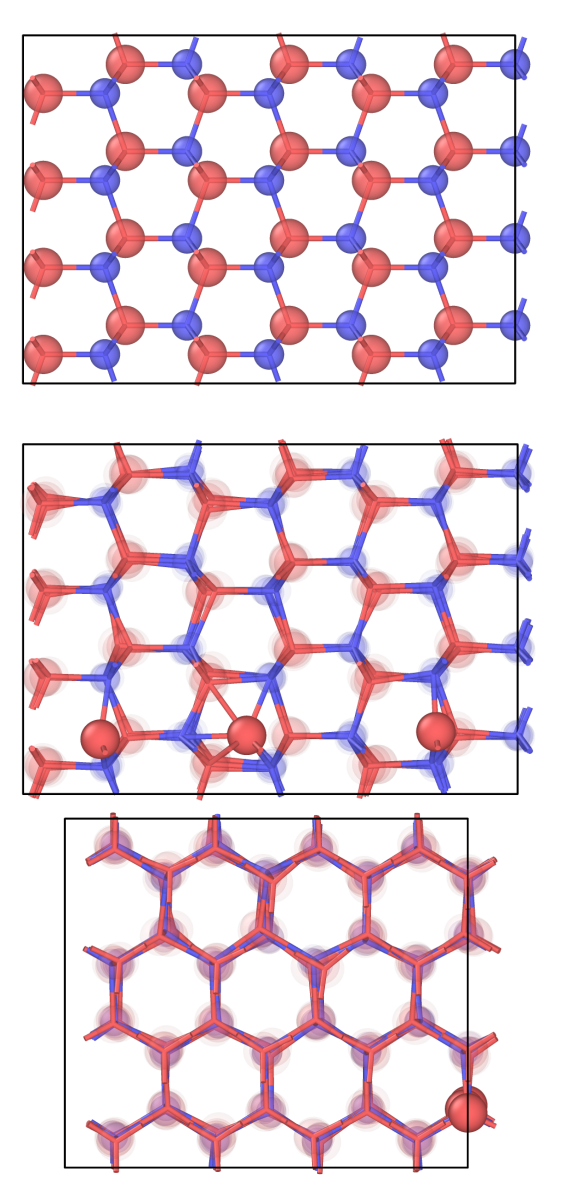
\includegraphics[width=\textwidth]{./data/plots/defects/186.02.AgI/defects_all.png}
	\caption{AgI viewed in (100) direction. Top: High-symmetry wurtzite structure. Middle: Silver ions (red) move into interstitial sites along (001) direction when $\sigmaA (t) \approx 1.3$. Bottom: The same configuration viewed along (001) direction.}
	\label{fig:defects.AgI.1}
\end{marginfigure} 
%
The time-resolved anharmonicity measure for AgI at 300\,K is shown in Fig.\,\ref{fig:defects.AgI}. As in $\gamma$-CuI, the value jumps back and forth between the already quite large reference value of $\sigmaA \approx 0.7$, short spikes at $\sigmaA \approx 0.5$, and longer periods where $\sigmaA \approx 1.3-1.6$ for several picoseconds. For example, the first trajectory displayed in Fig.\,\ref{fig:defects.AgI}~a) jumps between $\sigmaA \approx 0.7$ and $\sigmaA \approx 1.3$ several times, where the longest time span around this value is about 5\,ps. Averaging the positions over this time span as before, we obtain a supercell containing three Ag defects moving along (001) direction in the supercell, as shown in Fig.\,\ref{fig:defects.AgI.1} (middle and bottom), as opposed to the reference wurtzite structure (top).
It is again very likely that the instability of the wurtzite lattice towards defect formation at room temperature is a precursor of the actual phase transition taking place at temperatures approximately 120\,K higher. 

\newpage
\subsection{AgCl}
Silver chloride (AgCl) is yet another material of the class of transition metal halides, and the room-temperature stable phase is rock salt~\cite{Lowndes.1972,Andreoni.1983,Batchelor.1995}.
\begin{figure}
	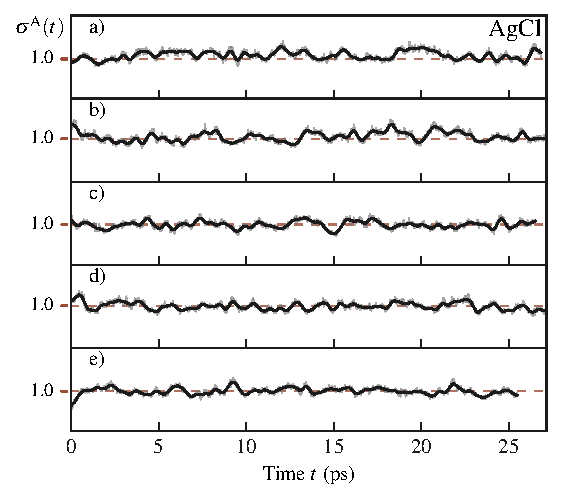
\includegraphics[width=\textwidth]{./data/plots/defects/225.02.AgCl/sigma_vs_time.pdf}
	\caption{Time-resolved anharmonicity measure $\sigmaA (t)$ for rock salt AgCl in five molecular dynamics runs of 30\,ps length. No temporarily increased value of $\sigmaA (t)$ is observed.}
%	\mscomment{pair distribution function?}
%	\FK{see Fig. \ref{fig:defects.pdf.agcl}}
	\label{fig:defects.AgCl}
\end{figure}
%
\begin{marginfigure}[-2in]
	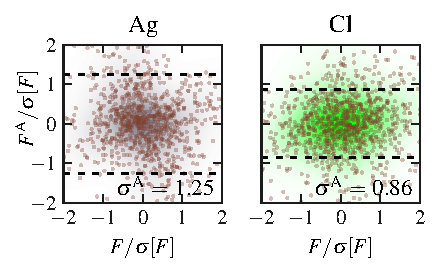
\includegraphics[width=\textwidth]{./data/plots/defects/225.02.AgCl/per_atom/histogram_atoms_margin.pdf}
	\caption{Species-resolved anharmonicity score in AgCl.}
	\label{fig:defects.AgCl.sigmaA}
\end{marginfigure}
%
As opposed to the previously discussed transition metal halides CuI and AgI, the time-resolved anharmonicity $\sigmaA (t)$ exhibits no ``jumps'' in AgCl, but rather stays close to $\sigmaA \approx 1$, which can be interpreted as a situation where the harmonic model loses predictive power for the observed forces.\footnote{$\sigmaA \approx 1$ signals a situation where the anharmonic contribution to the forces becomes as strong as the forces themselves.} By resolving the anharmonicity measure per atom species in Fig.\,\ref{fig:defects.AgCl.sigmaA} similar to the discussion for KCaF$_3$ in Sec.\,\ref{sec:anharmonicity_measure}, we see that the forces on chlorine atoms are better described by the harmonic model with $\sigmaA_{\rm Cl} = 0.86$ than those on silver with $\sigmaA_{\rm Ag} = 1.25$. 
%\mscorrect{performs?}
%\FK{is more predictive?}
This is in line with the previous observations in metal halides where small cations proved to be more mobile and susceptible to dislocations~\cite{Boyce.1979,Brenner.2020}. However, no clear-cut dislocation pattern can be identified for AgCl as opposed to CuI and AgI.
%
\begin{figure}
	\centering
	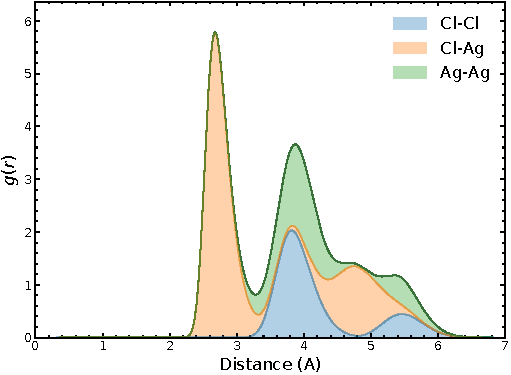
\includegraphics[width=3.5in]{./data/plots/pdfs/agcl.pdf}
	\caption{Pair discribution function for first four coordination shells of rock salt (SG\,225) AgCl.
%	Coordination shells: 
%	1: 2.75579 atoms: Cl-Ag 
%	2: 3.89727 atoms: Ag-Ag/Cl-Cl 
%	3: 4.77317 atoms: Ag-Cl 
%	4: 5.51158 atoms: Ag-Ag	
%	\mscorrect{fix!}
}
	\label{fig:defects.pdf.agcl}
\end{figure}
%
\newthought{The nature of the dynamical effects manifesting in AgCl can nevertheless be elucidated.} We do this by computing the pair distribution functions for the first four coordinates shells in AgCl~\cite{AllenTildesley}, as shown in Fig.\,\ref{fig:defects.pdf.agcl}, and contrasting them with the prototypical, largely harmonic rock salt material magnesium oxide (MgO, $\sigmaA = 0.17$) in Fig.\,\ref{fig:defects.pdf.mgo.small}. 
%
\begin{marginfigure}
	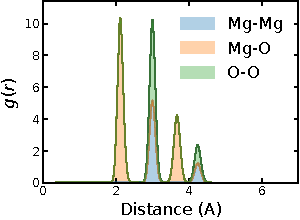
\includegraphics[width=\textwidth]{./data/plots/pdfs/mgo_small.pdf}
	\caption{Radial distribution function resolved by pair contributions.}
	\label{fig:defects.pdf.mgo.small}
\end{marginfigure}
%
In MgO, the distribution of atoms are narrowly distinguishable, which means that the atoms vibrate closely around their reference position, a typical feature of harmonic dynamics. 
%\mscomment{isn't this a sing of harmonic behavior?}
%\FK{Exactly.}
In AgCl on the other hand, only the first coordination shell of silver-chlorine atoms is distinct at 300\,K. The chlorine (Cl-Cl) and silver (Ag-Ag) sublattices (purple/green area in Fig.\,\ref{fig:defects.pdf.agcl}) show discernible peaks, although the broadening is significant compared to MgO. The silver-chlorine (Cl-Ag) distribution (yellow area) is even more broadened and is still non-zero at distances normally characteristic of like atoms (Cl-Cl or Ag-Ag) , see~e.\,g.,~the non-zero width of the yellow curve at 3.9 and 5.5\,\AA (second and fourth coordination shell). In total, this leads to a very strong broadening in the third and fourth coordination shell, with a barely discernible local maximum in the third coordination shell (4.8\,\AA).
This is in line with experimental Extended X-ray Absorption Fine Structure (EXAFS) measurements detecting an ``anomalously large motion'' in the third neighbor shell already at a temperature of 120\,K~\cite{Batchelor.1995}.
This hints at severe dynamical distortions throughout the simulation which are typically discussed in terms of dynamical Frenkel pair formation, where the mobile Ag$^+$ cations dynamically populate interstitial sites~\cite{Aboagye.1975,Andreoni.1983,Wilmer.1995,Mebane.2010}. While we can confirm an increased mobility of Ag$^+$ ions as discussed above, we do not observe a local accumulation of Ag$^+$ ions at interstitial sites, which should correspond to additional local maxima in the respective pair distribution functions compared to the reference structure. 
%
%\mscomment{minima? maxima?}
%\FK{maxima probably correct}
%\mscomment{where would interstitial be in Fig. 4.21?}
%\FK{check!}
%
However, such an effect might very well occur at higher temperatures, and the observed effects are fingerprints of the instability of the lattice towards this kind of dynamical defect formation.
Irrespective of the exact type of defect formation, %which is beyond the scope of this work, 
the observed dynamical effect hints at a strong form of premelting phenomenon in AgCl, which has an experimental melting temperature of 728\,K.

\newthought{Similar effects can be observed in silver bromide (AgBr)}. As discussed in Ref.\,\cite{Andreoni.1983}, the dynamical properties of AgCl and AgBr share many similarities with the chemically related material AgI presented in the previous section. In contrast to AgI however, they do not become superionic conductors before melting, despite the increased ion mobility presented here.
%\mscomment{this is not your results}
%\FK{true}

\section{Anharmonicity and Boltzmann transport}
\label{sec:anharmonicity.bte}
As previously mentioned, there are two established approaches to compute thermal conductivities in solids from first principles: Fully anharmonic Green Kubo simulations, and Boltzmann transport theory with perturbative treatment of phonon-phonon interactions. 

In order to assess the need for non-perturbative simulations, 
% even in simple materials, 
we have reproduced thermal conductivities calculated by a state-of-the-art Boltzmann transport approach published by Xia and coworkers in Ref.\,\cite{Xia.2020} in the light of the previously introduced anharmonicity measure $\sigmaA$ in Fig.\,\ref{fig:anh.bte}.
%
\begin{figure}
	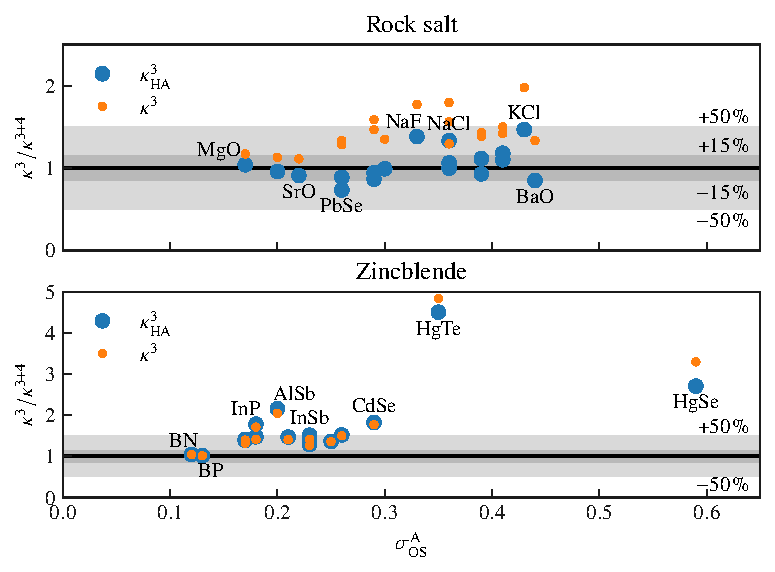
\includegraphics[width=4.1in]{./data/plots/BTE_comparison/k_34.pdf}
	\caption{
		Boltzmann transport calculation of thermal conductivity at room temperature including third- and fourth-order contributions to the potential-energy surface for 34 zinc blende and rocksalt compounds from Ref.\,\cite{Xia.2020}. $\kappa^3_{\rm HA}$: Boltzmann transport with three-phonon scattering rates computed from third-order terms, cf. Eq.\,\eqref{eq:Gamma_s}. $\kappa^3$: Boltzmann transport with three-phonon scattering and additionally accounting for phonon-frequency renormalization via self-consistent phonon theory~\cite{Xia.2018}. These approximations are compared with $\kappa^{3+4}$,~i.\,e.,~the highest available level of theory where both frequency renormalization and four-phonon scattering are additionally included in the computation of thermal conductivity. The data points give the relative change with respect to $\kappa^{3+4}$,~i.\,e.,~1 means perfect agreement between different levels of theory.
	}
	\label{fig:anh.bte}
\end{figure}

The figure shows a comparison of three different levels of perturbation theory employed in that work: i) $\kappa^3_{\rm HA}$ with three-phonon scattering computed from third-order force constants with harmonic dispersions, ii) $\kappa^3$, which includes the effect of phonon frequency renormalization at finite temperature, and iii) $\kappa^{3+4}$, where additionally four-phonon scattering from a fourth-order expansion of the potential-energy surface is accounted for~\cite{Ecsedy.1976,Feng.2016, Xia.2018}.\sidenote[][-4em]{The original nomenclature in Ref.\,\cite{Xia.2020} is $\kappa^{\rm Ha}_{\rm 3ph}$ for $\kappa^3_{\rm HA}$, $\kappa^{\rm SCPH}_{\rm 3ph}$ for $\kappa^3$, and $\kappa^{\rm SCPH}_{\rm 3,4ph}$ for $\kappa^4$.}
 We show the results from lower-level theory, $\kappa^3_{\rm HA}$ and $\kappa^3$, in comparison with the highest-available level, $\kappa^{3+4}$, by computing their ratio, and discuss the relative changes as function of one-shot $\sigmaA$ values from our anharmonicity screening~\cite{Knoop.2020}.\sidenote[][-4.5em]{Xia and coworkers investigated 19~rock~salt and 17~zincblende compounds~\cite{Xia.2020}, from which 18 (16) were included in our screening~\cite{Knoop.2020}.}\sidenote[][0em]{The computational details vary between the study conducted by Xia and coworkers in Ref.\,\cite{Xia.2020}, and our anharmonicity screening~\cite{Knoop.2020}. Most importantly, Xia and coworkers used the PBE xc-functional except for PbTe, AgCl, and HgTe, for which PBEsol was used~\cite{Perdew.1996,Perdew.2008}, whereas we used PBEsol for all materials. The data shown in Fig.\,\ref{fig:anh.bte} is therefore not fully consistent. Nevertheless, we expect no qualitative changes due to the xc-functional mismatch, since both functionals are of the GGA type with closely related parametrizations.}

The most harmonic rock salt material studied in Ref.\,\cite{Xia.2020}, MgO with $\sigmaAOS = 0.17$, shows good agreement between $\kappa^3_{\rm HA}$ and $\kappa^{3+4}$, with a 3.9\,\% increased value of $\kappa^3_{\rm HA}$ compared to $\kappa^{3+4}$. However, the agreement relies on the cancellation of opposite changes arising from the inclusion of frequency renormalization ($\kappa^3_{\rm HA} \to \kappa^3$), which increases the calculated thermal conductivity by 13\,\%, and fourth-order scattering ($\kappa^3 \to \kappa^{3+4}$), which subsequently reduces $\kappa$ by 15\,\%. This cancellation between frequency renormalization and fourth-order scattering is generally observed across the rock salt materials studied, and the differences tend to grow with increasing anharmonicity: In PbSe ($\sigmaAOS = 0.26$), temperature renormalization increases $\kappa^3_{\rm HA}$ by 82\,\%, whereas fourth-order scattering subsequently reduces $\kappa$ by 25\,\%, leading to a total increase of $\kappa$ by 36\,\% ($\kappa^3 \to \kappa^{3+4}$), or a 27\,\% underestimation of $\kappa^{3+4}$ by $\kappa^3_{\rm HA}$, respectively. The strongest deviation between $\kappa^3_{\rm HA}$ and $\kappa^{3+4}$ is seen for KCl ($\sigmaAOS = 0.43$), where $\kappa^3_{\rm HA}$ overestimates $\kappa^{3+4}$ by 47\,\%.

The general trend of error cancellation when going from $\kappa^3_{\rm HA}$ through $\kappa^{3}$ to $\kappa^{3+4}$ in rock salt materials is in line with the findings by Ravichandran and Broido in their study of NaCl with a closely related approach~\cite{Ravichandran.2018}.

\newthought{For the zincblende materials studied in Ref.\,\cite{Xia.2020},} we observe a different trend: For all materials besides the strongly anharmonic HgTe ($\sigmaAOS = 0.35$) and HgSe ($\sigmaAOS = 0.59$), the frequency renormalization has a negligible to small effect on the thermal conductivity, with a relative change of 0.3\,\% in the very harmonic BN ($\sigmaAOS = 0.13$), to 6.5\,\% in the mildly anharmonic InSb ($\sigmaAOS = 0.23$). Besides its mild effect on the dispersion, anharmonicity leads to four-phonon scattering of growing strength, so that the difference between $\kappa^3_{\rm HA}$ and $\kappa^{3+4}$ becomes significant,~e.\,g.,~for InP ($\sigmaAOS = 0.18$), where $\kappa^3_{\rm HA}$ overestimates $\kappa^{3+4}$ by 78\,\%. Already in AlSb with $\sigmaAOS = 0.20$, $\kappa^3_{\rm HA}$ is 115\,\% larger than $\kappa^{3+4}$, and in the most extreme case, HgTe, $\kappa^3_{\rm HA}$ is 4.5~times larger than the reference value $\kappa^{3+4}$, as discussed in detail in Ref.\,\cite{Xia.2020}.
These findings and trends are in line with a similar study conducted by Ravichandran and Broido on 17~zincblende compounds by a related Boltzmann transport approach~\cite{Ravichandran.2020}, although their findings do not agree quantitatively, partially due to different different xc-functionals.\footnote{Ravichandran and Broido use the local-density approximation for all materials.}\footnote{
  Xia and coworkers find consistently lower thermal conductivities, which can be explained by the different treatment of electronic structure as noted above, and other methodological differences. However, the ratio of computed thermal conductivities when using third vs. third and fourth order scattering is in good agreement for all materials~\cite{Xia.2020,Ravichandran.2020}.}
  
  \newthought{These findings show that higher-order anharmonicity can have significant impact on room-temperature thermal conductivities}, already in simple, mildly anharmonic materials (InP, AlSb), and change results drastically in strongly anharmonic materials (HgTe, HgSe). In cases where lowest-order perturbation theory predicts thermal conductivities in agreement with higher-order approaches, this is often due to error cancellation, as discussed for the rock salt materials~\cite{Ravichandran.2018}.

% REM: AlSb is ok, I confused lack of isotope scattering in Ravichandran's values (k_pure, pure for no isotope scattering). Xia uses isotope scattering throughout.



\section{Conclusion}

Using the anharmonicity measure $\sigmaA$ introduced in Sec.\,\ref{sec:anharmonicity.definition}, we have shown that anharmonicity defined in this way strongly correlates with bulk thermal conductivity in simple semiconductors and insulators. Based on this finding, we have suggested candidate thermal insulator materials for further study. In these materials, we have observed a variety of non-perturbative dynamical effects, and discussed them for the prototypical systems KCaF$_3$, $\gamma$-CuI, $\beta$-AgI, and AgCl. The common feature of these effects is that they reflect thermodynamic phenomena which are known to occur in the respective materials, but at significantly higher temperatures. This comprised the onset of structural phase transitions in KCaF$_3$, fingerprints of a superionic phase in CuI and AgI, and pre-melting phenomena in AgCl and AgBr. Although these phenomena are known, we have presented a new way of finding and discussing these effects in terms of the time-resolved anharmonicity measure $\sigmaA (t)$.
%\mscomment{what was your finding? embryos like this were known to exist before}
%\FK{not to me, but I'd be happy to find a reference and supplement previous findings}
%\mscomment{what does this mean for you project?}
%\FK{it means that these materials are particularly interesting to study -- but also particularly difficult to converge out and gather statistics.}

In the same light, we have scrutinized Boltzmann transport approaches for computing thermal conductivity. We found that higher-order anharmonicity can play an important role and lower thermal conductivity considerably, even in simple compounds at room temperature. This calls for the necessity of non-perturbative approaches, for two reason: First, the inclusion of fourth-order scattering cannot necessarily be considered sufficient when significant differences compared with third-order scattering are observed. Second, treating fourth-order terms is computationally very demanding and has hitherto only been performed for simple systems with high symmetry. When aiming for a consistent and accurate simulation of thermal conductivities across materials spaces containing more complex systems, non-perturbative calculations in terms of \emph{ab initio} Green Kubo simulations therefore seem necessary. In the next chapter, we introduce and benchmark this method, before applying it to materials from the list of candidates identified earlier.

%From a computational perspective, the two approaches have different strengths: Perturbative techniques are ideally suited when the anharmonicity is weak,~i.\,e.,~there is a well defined reference configuration and the harmonic terms in the potential dominate the dynamical evolution of the system. However, in strongly anharmonic systems, these basic assumptions can be violated, for example because the reference configuration changes qualitatively during phase transitions, or the anharmonic terms in the potential become too strong to be described by the asymptotic perturbation series~\cite[p.\,53]{NegeleOrland}. The Green-Kubo technique on the other hand does not require approximations to the potential-energy surface, and therefore naturally includes dynamical effects of arbitrary anharmonic strength. It is ideally suited in situations where the anharmonicity is strong,~i.\,e.,~when the basic assumptions of perturbation theory are not satisfied. It is therefore desirable to \emph{measure} the ``degree of anharmonicity'' to enable a discussion of anharmonicity on a quantitative basis.



% \chapter{Ab Initio Green Kubo: Implementation}
% \chapter{Ab Initio Green Kubo: Implementation}
\label{chp:implementation}
\newcommand{\tcut}{t_{\rm c}}
\newcommand{\teff}{t^{\rm eff}_0}

The theoretical background for the \emph{ab initio} simulation of thermal conductivity has been established in the previous chapters, in particular, Chp.~\ref{chp:heat_transport}. The purpose of this chapter is to discuss the practical implementation of the respective formulas. 

We restate the Green-Kubo formula for the thermal conductivity initially introduced in Sec.\,\TODO{ref} as
\begin{align}
	\kappa^{\alpha \beta} (T)
		= \int \d \Gamma_0 ~ \kappa^{\alpha \beta} (\Gamma_0) f_T (\Gamma_0) ~,
	\label{eq:implementation.kappa.avg}
\end{align}
where $\kappa^{\alpha \beta} (T)$ are the Cartesian components of the thermal conductivity tensor at temperature $T$, and $\Gamma_0$ are phase-space configurations with a respective ensemble weight $f_T (\Gamma_0)$ at the given temperature. For each phase-space configuration $\Gamma_0$, the thermal conductivity is computed as
\begin{align}
	\kappa^{\alpha \beta} (\Gamma_0)
		&=
		\frac{V}{k_{\rm B} T^2} 
		\lim_{t_{\rm c} \to \infty}
		\int_{0}^{\tcut} 
		\d t ~ C_{JJ}^{\alpha \beta} (\Gamma_0, t)~,
	\label{eq:implementatino.kappa.1}
\end{align}
where $	C^{\alpha \beta}_{J J} (\Gamma_0, t)$ denotes the heat flux autocorrelation function (HFACF),
\begin{align}
	C^{\alpha \beta}_{J J} (\Gamma_0, t)
		=
		\lim_{t_{0} \to \infty}
		\frac{1}{t_0 - t}
		\int_{0}^{t_{\rm 0} - t} 
		\d s ~ J^\alpha (\Gamma_{t + s}) J^\beta (\Gamma_s)~,
	\label{eq:implementatino.acf.1}
\end{align}
and a phase-space point $\Gamma_t$ is related to the initial configuration $\Gamma_0$ through the canonical time evolution determined by the many-body Hamiltonian of the system, $\mathcal H (\Gamma)$. Equation~\ref{eq:implementation.kappa.avg} through~\ref{eq:implementatino.acf.1} represent an exact reformulation of the Green Kubo formula.


\newthought{In order to evaluate these equations in finite simulations}, the integrals need to be discretized and truncated to finite domains. First, we approximate Eq.\,\eqref{eq:implementation.kappa.avg} by choosing a finite set of starting configurations $\Gamma_0^i$, so that
\begin{align}
	\kappa^{\alpha \beta} (T)
		\approx
		\frac{1}{N} \sum_{i=1}^N \kappa^{\alpha \beta} (\Gamma_0^i)~,
	\label{eq:implementation.kappa.mean}
\end{align}
where the starting conditions $\Gamma_0^i$ are chosen from NVT molecular dynamics simulations for the thermodynamic conditions of interest. For each starting condition $\Gamma_0$, we perform NVE molecular dynamics simulations to generate the time evolution of the system, $\Gamma_t$, and evaluate the heat flux, $J^\alpha (\Gamma_t)$ along this trajectory. The simulation is performed for a total simulation time $t_0$, thereby truncating the time integral in Eq.\,\eqref{eq:implementatino.acf.1}. From resulting autocorrelation function of finite length, the thermal conductivity is computed via Eq.\,\eqref{eq:implementatino.kappa.1}, where a \emph{cutoff time} $\tcut < t_0$ is chosen to reduce noise when the autocorrelation function has effectively decayed~\cite{Jones2012}.
After computing the thermal conductivity for each trajectory, the final value is given by Eq.\,\eqref{eq:implementation.kappa.mean},~i.\,e.,~by the \emph{mean} of the individual trajectories. The statistical error due to the finite ensemble average is estimated by the \emph{standard error},~i.\,e.,~the standard deviation of the mean,
\begin{align}
	\Delta \kappa^{\alpha \beta} (T)
		= \frac{1}{\sqrt{N}} \sqrt{\frac{1}{N} \sum_i \left( \kappa^{\alpha \beta} (T) - \kappa^{\alpha \beta} (\Gamma_0^i) \right)^2}~.
	\label{eq:imp.kappa.err}
\end{align}


\REM{Discuss $\kappa = \frac{1}{3} \sum_{\alpha} \kappa^{\alpha \alpha}$}


\newthought{In empirical force field approaches}, the appearing equations are typically evaluated as is, and convergence in size and time can be checked in a brute-force way by increasing the respective scales well beyond the necessary limits\CITE{Lammps, Jones, more}. From an \emph{ab initio} perspective, the accessible size and time scales are each at least two orders of magnitude lower,\footnote{Force fields: 1\,ns for 10000~atoms within 1 day, \emph{ab initio}: 50\,ps for 200~atoms within 1~months.} and additional steps are necessary to increase the amount of information that can be extracted from the comparatively short simulations. The purpose of this chapter is to discuss these additional steps in detail: First, we present steps to remove noise from the heat flux autocorrelation functions $C_{JJ} (t)$, which enables to choose cutoff times $\tcut$ in a numerically robust way. Next, we discuss the size extrapolation scheme in terms of the harmonic mapping presented in Sec.\,\ref{sec:aiGK} which allows to correct for the finite size of simulations cells used in \emph{ab initio} molecular dynamics simulations. Finally, we discuss the necessary simulation times $t_0$ and how those can be estimated for novel materials.

\REM{Case study MgO which is fairly harmonic, apply to strongly anharmonic CuI}

\section{Noise Reduction Scheme}
\subsection{Discard non-contributing terms}
The raw \emph{ab initio} heat flux used in this work was defined in Eq.\,\eqref{eq:J_ai} and is given for a phase-space point $\Gamma_t = \set{{\bf R} (t), \dot{\bf R} (t)}$ by
\begin{align}
	{\bf J}^{\rm raw} (t) = \sum_I \sigma_I (t)  \dot{\bf R}_I (t)~,
	\label{eq:imp.J.0}
\end{align}
where $\sigma_I (t) \equiv \sigma_I [{\bf R} (t)]$ are atomic virial tensors for the configuration at the given time $t$ as defined in Eq.\,\eqref{eq:hf.sigma_I}, and $\dot{\bf R}_I (t)$ is the velocity of atom $I$ as usual. We split the raw flux in two parts,
\begin{align}
	{\bf J}^{\rm raw} (t)
		= \sum_I \delta \sigma_I (t) \dot{\bf R}_I (t) 
		+ \sum_I \braket{\sigma_I} \dot{\bf R}_I (t)~,
	\label{eq:imp.J.1}
\end{align}
where $\braket{\sigma_I}$ is the average atomic virial, and $\delta \sigma_I (t)$ is the time-dependent part. In the absence of diffusion, the second term is the total time derivative of a bounded vector field, $\sum_I \braket{\sigma_I} \dot{\bf R}_I (t) = \frac{\d}{\d t} \sum_I \braket{\sigma_I} {\bf R}_I (t)$. By means of the gauge invariance principle introduced in Sec.\,\ref{sec:gauge_invariance}, it therefore does not contribute to the time integral in Eq.\,\eqref{eq:implementatino.kappa.1}, and can be discarded before evaluating the heat flux autocorrelation function~\cite{Ercole2016}. We therefore always use the following heat flux expression in the following:
\begin{align}
	{\bf J} (t)
		= \sum_I \delta \sigma_I (t) \dot{\bf R}_I (t)~.
	\label{eq:imp.J}
\end{align}
Depending on the material, discarding the non-contributing part from the raw heat flux reduces the noise in the simulation \emph{massively}, as shown for the case of MgO in the upper panel of Fig.\,\ref{fig:imp.hfacf.kappa.1} (orange curves compared to light blue curves).
\begin{figure}
	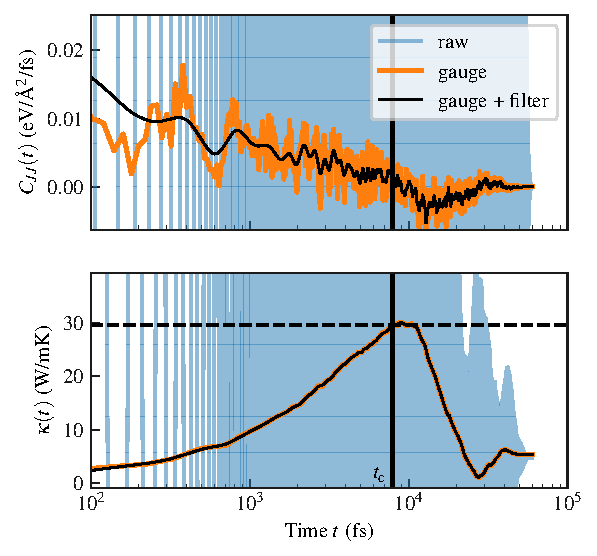
\includegraphics[width=\textwidth]{./data/plots/implementation/MgO/hfacf_data_yy_3.pdf}
	\caption{Heat flux autocorrelation function $C_{JJ}(t)$ (HFACF) as defined in Eq.\,\eqref{eq:implementatino.acf.1} and its cumulative integral,~i.\,e.,~the thermal conductivity $\kappa (t)$ as function of lag time $t$. Light blue: $C_{JJ}(t)$ and $\kappa (t)$ obtained by using the raw flux as defined in Eq.\,\eqref{eq:imp.J.0}. Orange: After discarding the gauge-invariant term in Eq.\,\eqref{eq:imp.J.1}. Black curves: After applying additional, integral-preserving noise filtering as explained in the main text. The cutoff time $t_{\rm c}$ is chosen based on the ``first dip'' of the noise-filtered HFCAF.
	\emph{Computational details:} The shown data is for the $\kappa^{yy}$-component of MgO in an aiMD simulation of 60\,ps total length using a time step of 5\,fs. The heat flux was evaluated every four steps. The system was thermalized to 300\,K using a Langevin thermostat. The system size is 216 atoms in a cubic supercell.}
	\label{fig:imp.hfacf.kappa.1}
\end{figure}

\subsection{Noise filtering}
After discarding the gauge-invariant contributions from the heat flux, there is still a considerable level of noise in the HFACF, which hinders a robust identification of the time at which it is fully decayed,~i.\,e.,~the cutoff time $\tcut$. We investigated several techniques to identify cutoff times, however, most of the available techniques such as the first avalanche technique introduced in Ref.\,\cite{Chen2010} are not fully parameter-free, and need hand tuning, even if very little.\footnote{The first avalanche technique determines cutoff times by means of a signal-over-noise ratio and relies on two parameters, a window size for computing moving averages, and a threshold value for the resulting avalanche function.} We therefore suggest an approach that does only rely on a single parameter which is chosen based on the vibrational spectrum of the material: Motivated by the fact that the \emph{integrated} HFACF,~i.\,e.,~the cumulative thermal conductivity
\begin{align}
	\kappa (t)
		=
		\frac{V}{k_{\rm B} T^2} 
		\int_{0}^{t} 
		\d t' ~ C_{JJ} (t')~,
	\label{eq:imp.kappa.cum}
\end{align}
is already a much smoother function than the HFACF itself, we apply a shape-preserving Savitzky-Golay filter to $\kappa (t)$~\cite{Savitzky1964}. The remaining parameter is the window size for the filter. It is chosen based on the vibrational spectrum of the material by taking the period length corresponding to the slowest significant frequency $\omega_{\min}$. Thereby, all noise of higher frequency is effectively filtered from $\kappa (t)$, while all relevant time integrals are preserved by construction. The filter is constructed such that the antisymmetry of $\kappa (t)$ in time, $\kappa (-t) = - \kappa (t)$ is respected.\footnote{The antisymmetry of $\kappa (t)$ is a consequence of the time symmetry of $C_{JJ} (t)$.} This also ensures that $\kappa (t)$ vanishes identically at $t=0$.

Based on the filtered cumulative thermal conductivity, the HFCAF can be obtained by differentiating, which carries over the filtering to $C_{JJ} (t)$. The filtered HFACF can be obtained analytically by fitting spline functions to $\kappa (t)$, or numerically by applying the same filter on the numerical gradient of $\kappa (t)$. The resulting cumulative thermal conductivity $\kappa (t)$ and HFACF $C_{JJ} (t)$ are shown as black curves in Fig.\,\ref{fig:imp.hfacf.kappa.1}. From the noise-filtered HFACF, the cutoff time $\tcut$ is chosen by a ``first dip'' criterion,~i.\,e.,~when $C_{JJ} (t)$ drops to zero~\CITE{Chen2010 and references therein}. This corresponds to the first significant plateau in $\kappa (t)$ after removing the noise. With the cutoff time $\tcut$, the resulting thermal conductivity for a given component of the thermal conductivity tensor is given by the value $\kappa = \kappa (\tcut)$.

\newthought{The presented scheme} will be used for all reported values of thermal conductivity in the following.

\section{Size extrapolation}
\label{sec:imp.extrapolation}

After we have seen how the Green-Kubo formula is used to compute thermal conductivities from the \emph{ab initio} heat flux evaluated along aiMD trajectories, we shortly review the size extrapolation scheme discussed in more detail in Sec.\,\ref{sec:aiGK}. The aim of the size extrapolation is to correct for finite size effects occuring in aiMD simulations, because the supercells used in \emph{ab initio} simulations are limited in size, and phonon modes of longer wavelength than the supercell are therefore not included. 

\newthought{As discussed in Sec.\,\ref{sec:aiGK}}, the correction works by computing the harmonic contribution to the thermal conductivity $\kappa_{\rm ha}$ within the supercell via Eq.\,\eqref{eq:ha.kappa.bte}
\begin{align}
	\kappa_{\rm ha}^{\alpha \beta} = V k_{\rm B} \sum_{b, {\bf q}} v^\alpha_b ({\bf q}) v^{\beta}_b ({\bf q}) \fD \tau_b ({\bf q})~,
	\label{eq:imp.K.bte}
\end{align}
where $v_b^\alpha ({\bf q})$ is the group velocity of a phonon mode with band index $b$ and \emph{commensurate} wave vector $\bf q$, and $\tau_b ({\bf q})$ is the lifetime obtained from the autocorrelation function of the mode-resolved energy $E_b ({\bf q}, t)$ as defined and discused in Eq.\,\eqref{eq:G_s}~\cite{Carbogno2016}. For a given simulation $\set{\Gamma_t}$, Eq.\,\eqref{eq:imp.K.bte} is evaluated for all commensurate $\bf q$-points, and projected to the symmetry-inequivalent points the Brillouin zone as determinded by the space group operations to improve the statistics~\cite{Maradudin1968,Spglib}.

\newthought{In the next step}, the lifetimes $\tau_b ({\bf q})$ are interpolated to denser $\bf q$-point meshes by $\fD{\tilde{\tau}}_b (\tilde{\bf q}) = \fD \lambda_b (\tilde {\bf q}) \omega_b^{-2} (\tilde {\bf q})$ with a weakly $\bf q$-dependent function $\lambda_b (\tilde {\bf q})$ obtained by linearly interpolating the lifetimes obtained at commensurate $\bf q$-points. The scaling of lifetimes with $\omega_b^{-2} ({\bf q})$ is rooted in basic phonon theory as discussed in detail by Herring~\cite{Herring1954}. For the acoustic modes at ${\bf q} = \Gamma = 0$, where $\omega ({\bf q \to 0}) \to 0$, the value for $\lambda_b (\Gamma)$ is obtained by averaging over values at the surrounding $\bf q$-points. For the new, denser grid, an interpolated value,
\begin{align}
	\kappa_{\rm ha - int}^{\alpha \beta} (N_{\tilde{\bf q}}) = V k_{\rm B} \frac{N_{\bf q}}{N_{\tilde{\bf q}}} \sum_{b, \tilde{\bf q}} v^\alpha_b (\tilde{\bf q}) v^{\beta}_b (\tilde{\bf q}) \fD{\tilde{\tau}}_b (\tilde{\bf q})~,
	\label{eq:imp.K.bte.correction}
\end{align}
can be obtained, where $N_{\tilde{\bf q}}$ is the number of points in the new grid, and the factor $N_{\bf q} / N_{\tilde{\bf q}}$ accounts for the increased number points. The bulk limit of Eq.\,\eqref{eq:imp.K.bte.correction} is obtained by computing interpolated values for an increasing density of $\bf q$-points. Since Eq.\,\eqref{eq:imp.K.bte.correction} is a Riemann sum approximating the Brillouin zone integral $\int \d^3 q$, its convergence can be expected to be linear in $N_{\tilde{\bf q}}^{-1/3} \equiv 1 / n_q$,~i.\,e.,~the inverse number of $\bf q$-points per Cartesian direction. The slope of this curve can be used to extrapolate the value of $\kappa_{\rm ha}$ to bulk limit, as shown in Fig.\,\ref{fig:imp.kappa.bte.correction}.
\begin{figure}
	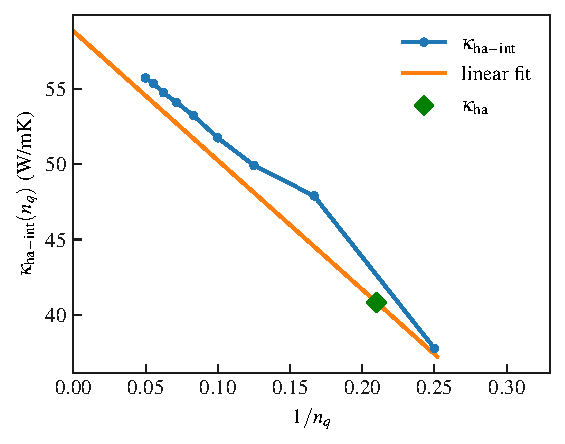
\includegraphics[width=.8\textwidth]{./data/plots/lifetimes/greenkubo_summary_interpolation_fit.pdf}
	\caption{Description of figure}
	\label{fig:imp.kappa.bte.correction}
\end{figure}
With the extrapolated value $\kappa_{\rm ha-bulk}$, a correction can be obtained via
\begin{align}
	\delta \kappa_{\rm ha-correction} 
		= \kappa_{\rm ha-bulk} - \kappa_{\rm ha}~,
	\label{eq:imp.K.correction}
\end{align}
from which the final result for the thermal conductivity can be obtained via
\begin{align}
	\kappa^{\alpha \beta}_{\rm corrected}
		 = \kappa^{\alpha \beta} + \delta \kappa^{\alpha \beta}_{\rm ha-correction}~,
	\label{eq:imp.K.corrected}
\end{align}
where $\kappa^{\alpha \beta}$ is the value from the \emph{ab initio} Green Kubo simulation.

\section{Simulation Time Convergence}
After we have seen how the cutoff time $\tcut$ in Eq.\,\eqref{eq:implementatino.kappa.1} can be obtained, and finite-size errors can be corrected, we discuss the convergence of presented scheme as a function of the simulation time $t_0$ in Eq.\,\eqref{eq:implementatino.acf.1}. We do this for the case of MgO for three independent trajectories of 60\,ps length each at GGA level of theory using the PBEsol function and light-default basissets in FHI-aims~\CITE{PBEsol, aims}. We truncate every trajectory in 10\,\% steps down to a length of 6\,ps, and apply the workflow presented in the previous chapters to each of the truncated trajectories. 
\begin{figure}
	\includegraphics[width=\textwidth]{./data/plots/kappa_convergence/examples/{225.02.MgO}.pdf}
	\caption{Thermal conductivity $\kappa$ as function of the effective simulation time $\teff = 7.5\,{\rm THz} \cdot t_0$ as defined in Eq.\,\ref{eq:imp.teff}. Values are given as the ensemble average over three independent trajectories. The error bars are computed according to Eq.\,\eqref{eq:imp.kappa.err} as the standard error of the ensemble average. The blue curve is a logistic curve defined in Eq.\,\eqref{eq:imp.f_logistic} fitted to the $\kappa$ values, the dashed blue curve is the infinite time limit of the fitted function. Gray dots represent the thermal conductivity as given by the simulation without the size-correction scheme.
	
	Please note that the values for $\kappa$ shown here cannot be directly compared to the value displayed in Fig.\,\ref{fig:imp.hfacf.kappa.1} or \ref{fig:imp.kappa.bte.correction}, because the latter only show single components of single runs, which can vary substantially from the total average.}
	\label{fig:imp.kappa.convergence.MgO}
\end{figure}

\newthought{The convergence of the final value of thermal conductivity} is shown in Fig.\,\ref{fig:imp.kappa.convergence.MgO} as function of a dimensionless \emph{effective simulation time} $t_0^{\rm eff}$, which we define via
\begin{align}
	\teff = t_0 \cdot \bar{\omega}_{\rm min}~,
	\label{eq:imp.teff}
\end{align}
where $t_0$ is the (truncated) simulation time, and $\bar{\omega}_{\rm min}$ is a characteristic frequency for the slow degrees of freedom of the system, chosen as the mean frequency of the lowest 20\,\% of the vibrational spectrum as explained in Fig.\,\ref{fig:imp.w_eff}. In MgO, this frequency is 7.5\,THz.
\begin{marginfigure}
	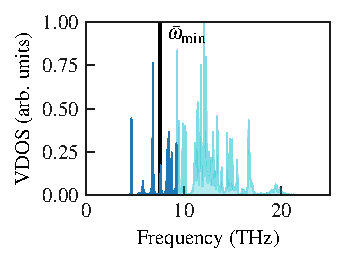
\includegraphics[width=\textwidth]{./data/plots/kappa_convergence/t_eff/vdos.pdf}
	\caption{Vibrational density of states (VDOS) for MgO. Light blue is the entire VDOS, solid blue is the lowest 20\,\% of the spectrum. $\bar{\omega}_{\rm min}$ is calculated as the average frequency in the low part of the spectrum.}
	\label{fig:imp.w_eff}
\end{marginfigure}
Figure~\ref{fig:imp.kappa.convergence.MgO} shows that the thermal conductivity converges after an effective simulation time of $\teff \approx 300$, which corresponds to a time of 40\,ps, where the value of $\kappa$ reaches a plateau within the error bars. The overall shape of the curve can be described as follows: Simulations shorter than 20\,ps ($\teff \lesssim 150$) sample the early decay of the HFACF which contribute about 30\,W/mK to the total thermal condcutivity. After a simulation time of 25\,ps ($\teff \gtrsim 190$), the late decay of the HFACF is sampled, contributing more than double the amount to the total thermal conductivity of $68.8 \pm 6.1$\,W/mK after the total simulation time. In the plot, this two-step behavior is approximated by a logistic function 
\begin{align}
	f(t) 
		= \frac{L}{1 + \exp \left(-\frac{(t-t_{\rm inflection})}{\tau} \right)} + f_0~,
	\label{eq:imp.f_logistic}
\end{align}
which allows to accurately quantify the simulation times where the second super-linear increase in $\kappa$ occurs,~i.\,e.,~the region in the vicinity of the inflection point located at $t_{\rm inflection} = 218$, which corresponds to a simulation time of 29\,ps.

The plot furthermore shows the thermal conductivities obtained without the finite-size correction discussed earlier as gray dots. Without this correction, the final value would be $45.5 \pm 6.1$\,W/mK. The finite-size correction therefore increases this value by about 50\,\%.

\section{Comparison to Experiment}


% \chapter{Thermal Conductivities for Strongly Anharmonic Compounds}
% \label{chp:results}

After introducing the implementation of the \emph{ab initio} Green Kubo (aiGK) method in the previous chapter, we are now in position to present results for the set of potential thermal insulators identified in chapter~\ref{chp:anharmonicity}.

We first discuss the question of simulation time convergence for an initial set of materials in order to predict systems which can be computed with a simulation time of 30-60\,ps. This time was chosen as a compromise between the finite amount of available computational ressources and the desire to compute as many materials from the list of candidates as possible.
% 57 materials
%
In a second step, we compare the computed thermal conductivities at room temperature to experimental references for the subset of materials for which experiments are available to further verify the aiGK method beyond the two materials presented in the previous chapter.
% 22 materials 
%
In the last step, we present the computed thermal conductivities for the remaining materials,~i.\,e.,~those for which no experimental thermal conductivity was reported before, and discuss how they fit into the schema of predicting thermal insulators from anharmonicity estimates as discussed in Sec.\,\ref{sec:kappa_vs_sigmaA}. We eventually highlight the particularly interesting class of chalcopyrite compounds and try to answer some open questions from experimental and semi-empirical theoretical literature.

% \idea{compare to theoretical approaches, i.e., the Roekeghem perovskites}



\section{Convergence estimation}
We discuss simulation time convergence in the light of the \emph{effective simulation time} introduced in Sec.\,\ref{sec:implementation.convergece}. The key idea is to identify lower boundaries for the \emph{necessary} effective simulation time in a material in order to asses whether a time-converged thermal conductivity is possible to obtain within a simulation time of 30-60\,ps. For choosing these boundaries, we leverage the observed convergence behavior of seven materials,~i.\,e.,~MgO, NaF, KMgF$_3$, NaCl, NaBr, CuI, and NaI, each of them computed with 60\,ps simulation time. We thereby define four thresholds of minimal effective simulation time based on a material's anharmonicity $\sigmaA$, reflecting that phonons in harmonic materials like MgO have longer lifetimes than those in anharmonic materials. The criteria are displayed in Fig.\,\ref{fig:results.convergence}. In particular, we define the thresholds $\teff > 240$ for harmonic materials with $\sigmaA \leq 0.2$, $\teff > 120$ for materials with $0.2 < \sigmaA \leq 0.3$, $\teff > 60$ for materials with $0.3 < \sigmaA \leq 0.4$, and $\teff > 45$ for materials with $\sigmaA > 0.4$.

%The rational for this approach is that for individual materials, one would always compute several times longer trajectories to ensure that all relevant contributions are captured. In turn, several times less materials could be computed with a given amount of computational resources. Here, we leverage observations across different materials to circumvent this necessity for individual materials, thereby allowing to compute good estimates for thermal conductivity for dozens of them.
%
\begin{figure}
	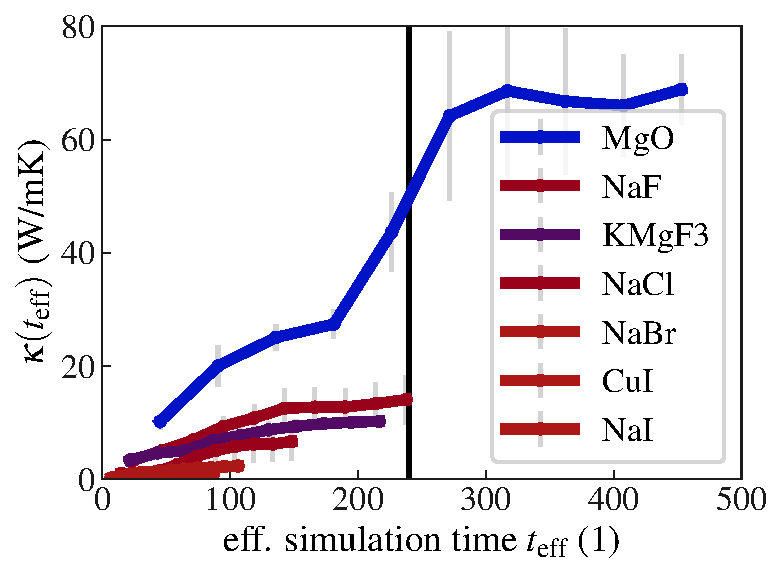
\includegraphics[width=.49\textwidth]{./data/plots/kappa_convergence/3.pdf}
	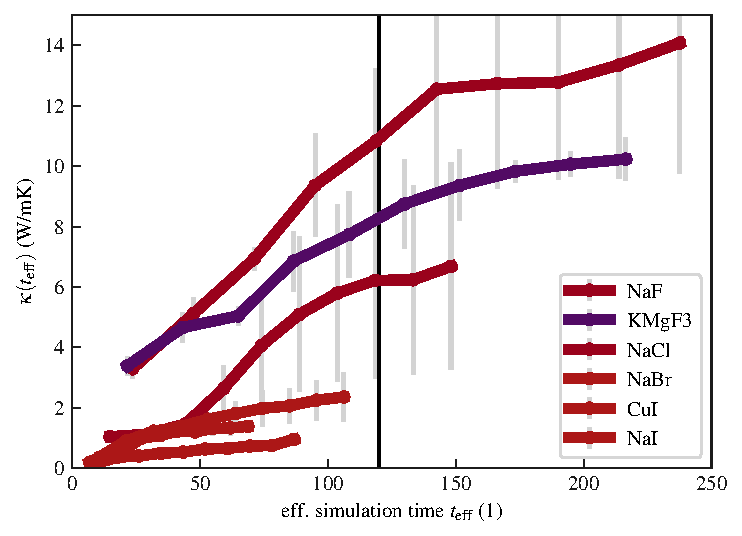
\includegraphics[width=.49\textwidth]{./data/plots/kappa_convergence/4.pdf}
	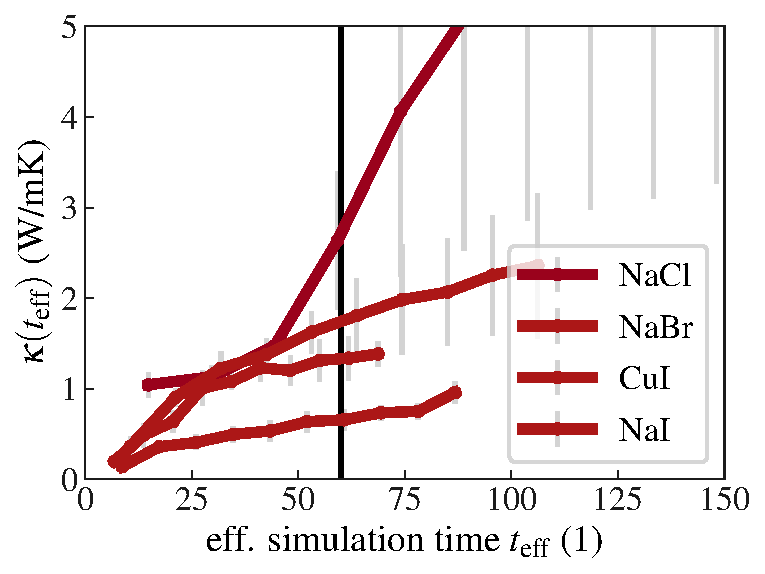
\includegraphics[width=.49\textwidth]{./data/plots/kappa_convergence/5.pdf}
	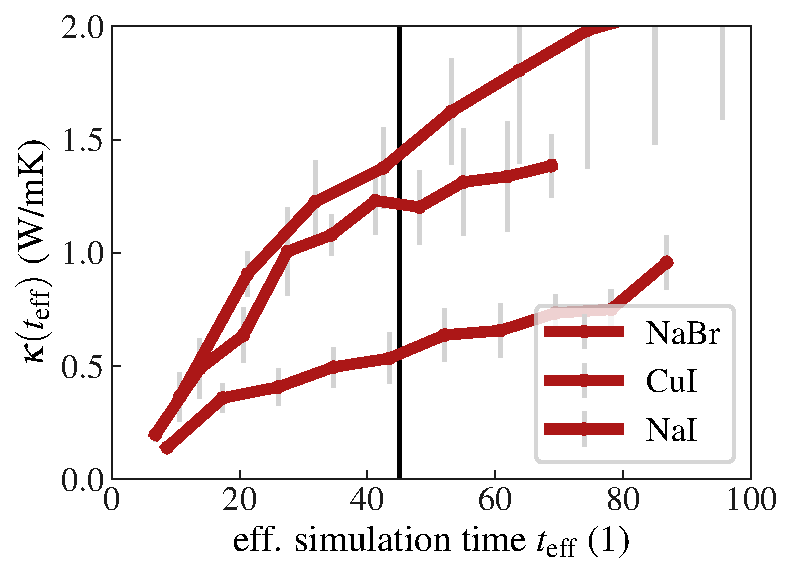
\includegraphics[width=.49\textwidth]{./data/plots/kappa_convergence/6.pdf}
	\caption{Illustration of minimal necessary effective simulation times. Upper left: $\teff = 240$ for harmonic materials with $\sigmaA \leq 0.2$. Upper right: $\teff = 120$ for materials with $0.2 < \sigmaA \leq 0.3$. Lower left: $\teff = 60$ for materials with $0.3 < \sigmaA \leq 0.4$. Lower right: $\teff = 45$ for materials with $\sigmaA > 0.4$.}
	\label{fig:results.convergence}
\end{figure}
%
We point out that at this stage, the given thresholds are meant as a \emph{necessary} condition for convergence, which ensures that a significant contribution to the cumulative thermal conductivity is included in the simulation. A statement about the \emph{sufficient} simulation time, however, can only made on the level of individual trajectories by means of longer simulation times. This verification should therefore be reserved for materials that show interesting properties after the \emph{necessary} simulation time.

Based on this estimation, we identify 57~materials out of the list of 112~candidates to compute thermal conductivity on, and discuss those in the following: First we compare thermal conductivities for 24 of these 57 materials to the experimental literature in order to benchmark the aiGK method, afterwards we present and discuss our findings for the remaining 33 materials without experimental reference.
\TODO{list of materials in appendix}



\section{Comparison to Experiment}
\label{sec:results.experiments}
In order to asses the validity of the aiGK method for the computation of thermal conductivity in anharmonic compounds, we compare results for 21 materials to the experimental literature. A detailed list including all considered experimental references is given in Tab.\,\ref{tab:kappa.exp} in appendix~\ref{sec:app.experiments}. The difficulties when comparing to experimental references have been discussed in detail for periclase MgO in Sec.\,\ref{sec:mgo.experiments}. In principle, these carry over to all other compounds, however, for most materials, the body of literature is much smaller compared to MgO. The list of experiments also includes measurements on polycrystalline samples. While thermal conductivity should be reduced in polycrystalline samples compared to single crystals because of boundary scattering, experimental studies have shown that the effect is minor in sufficiently dense polycrystalline samples, especially in low thermal conductivity materials which are less sensitive to boundary scattering due to their intrinsically low phonon mean free paths~\cite{Charvat.1957}. In the course of our literature review we have generally found differences of 0-20\,\% between measurements on single- and polycrystalline samples, which supports this finding. Nevertheless, additional care must be taken when evaluating literature on polycrystalline samples: Experiments aiming at measuring other properties besides thermal conductivity, in particular the thermoelectric figure of merit $zT$, typically do not attempt to reproduce the bulk thermal conductivity, and use less dense samples, which is beneficial for reducing thermal conductivity and thereby increasing the figure of merit. The resulting thermal conductivity will then be determined mostly by the details of the sample processing, 
%\mscomment{this is true for all experimental data}
%\FK{I disagree, actual bulk properties are somewhat robust against minor manufacturing differences. Clarify: I mean here that sampling process \emph{significanlty} determines the properties beyond single-digit deviations.}
and a comparison to bulk thermal conductivity is not meaningful. However, some experiments specifically aim at reproducing polycrystalline samples of near-bulk density in order to assess the bulk thermal conductivity of a material. Only experiments on polycrystalline samples of this type are considered in this work.

A comparison of thermal conductivities computed via the aiGK method as introduced in the previous chapter and the experimental literature is shown in Fig.\,\ref{fig:kappa_exp}.
%
\begin{figure}
	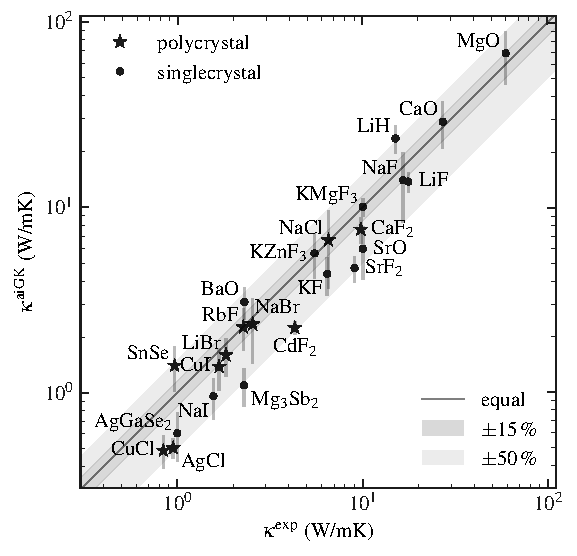
\includegraphics[width=\textwidth]{./data/plots/kappa_vs_exp_trusted/kappa_vs_exp_corrected_annotated.pdf}
	\caption{Comparison to experiment. Bullets($\bullet$): Single crystal. Stars ($\star$): Contains data from polycrystalline experiment. Error bar in y-direction: Statistical uncertainty for $\kappa^{\rm aiGK}$ from standard error over individual trajectories. Diagonal line: Agreement with experiment or mean of experiments if multiple available. Dark grey region: Agreement between mean experiment and mean computation with $\pm 15\,\%$ deviation. Light grey region: Agreement between mean experiment and mean computation with $\pm 50\,\%$ deviation.}
	\label{fig:kappa_exp}
\end{figure}
%
Overall, we find very good agreement in the 24 considered materials, with 10 out of 24 being within experimental accuracy of $\pm 15\,\%$, and all other within an extended %experimental 
accuracy which we choose as $\pm 50\,\%$ within the average experimental reference, reflecting the high degree of variation in experimental values for materials where a significant amount of references is available, see our discussion for MgO in Sec.\,\ref{sec:mgo.experiments} and the discussion in Ref.\,\cite{Wei.2016}. 

\begin{marginfigure}
	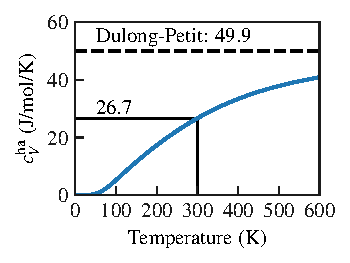
\includegraphics[width=\textwidth]{./data/plots/heat_capacity/225.LiH/thermal_properties.pdf}
	\caption{Harmonic heat capacity per formula unit $c_V^{\rm ha}$ for LiH compared to the classical Dulong-Petit value.}
	\label{fig:LiH.cv}
\end{marginfigure}
%
The strongest deviation from experiment is seen for LiH, which is computed as $\kappa^{\rm aiGK} = 23.6 \pm 4.0$\,W/mK, where the available experimental value is $\kappa^{\rm exp} = 14.7$\,W/mK~\cite{Slack.1973}. However, both lithium and especially hydrogen are light elements, so that LiH is not fully classical at room temperature, as can be estimated by comparing the harmonic heat capacity of LiH at 300\,K to the classical Dulong-Petit value in Fig.\,\ref{fig:LiH.cv}~\cite{Dove}. The harmonic heat capacity for LiH is only at about 50\,\% of the classically expected value of $6 R = 49.9$\,J/mol/K for solids with two atoms in the unitcell. This value can only be taken as an upper boundary to the deviation in thermal tranpsort properties expected from the lack of nuclear quantum effects, since low-frequency phonon modes already behave more classical at the given temperature~\cite{Volz.2020,Volz.2020b}. A significant overestimation by the classical Green Kubo method can nevertheless be expected in this material.\footnote{We evaluated several schemes to quantitatively correct for nuclear quantum effects~\cite{Wang.1990,Maiti.1997}, however, the literature seems to agree that this is an open problem for thermal conductivity in bulk solids, see in particular discussions in Ref.~\cite{Turney.2009,Puligheddu.2019}.}
%\mscomment{There have been efforts to estimate ZP/NQE effects, why wouldn't this improve the estimate?}
%\FK{The approaches I found were dealing with elemental solids. Li is 7 times heavier than H, so uniform scaling e.g. by correcting the temperature based on the heat capacity would, from my point of view, do more harm than good. It would give a correction into the right direction for the not-so-right reasons.}
Interestingly, the aiGK value agrees very well with another computational study by Lindsay, who found a value of $\kappa = 23.00$\,W/mK using third-order Boltzmann transport~\cite{Lindsay.2016}.\footnote{Lindsay used an LDA exchange-correlation functional, which thermal conductivity can deviate $\pm 20\,\%$ from the PBEsol functional used in this work~\cite{Carbogno.2016}. However, the disagreement with experiment is still significantly larger then the potential inaccuracy stemming from the xc functional.} In that approach, the quantum nature of nuclei should be better captured than in the aiGK method, and Lindsay ascribes the deviation from experiment to higher-order phonon-phonon interactions neglected in their approach. This discussion is in line with the more phenomenological discussion proposed by Slack in Ref.\,\cite{Slack.1973}, where he points out the strong anharmonicity in LiH that manifests in the change of phonon frequencies as measured by the Gr\"uneisen parameter. Indeed, in our study we find a value of $\sigmaA = 0.30$ for the strength of anharmonicity in LiH, which can be expected to be even larger when nuclear quantum effects are considered.\footnote{Nuclear quantum effects increase the anharmonic strength of LiH at room temperature by about 20\,\%~\cite{hengst1}.} We therefore suggest LiH as an interesting yet simple candidate for studying the interplay of strong anharmoncity and nuclear quantum effects in bulk solids in future work.

Another noteworthy material in the list is SnSe: We predict the thermal conductivity of SnSe to be $1.40 \pm 0.38$\,W/mK, which is on the upper limit of the experimental references and agrees reasonably with the measurements by Wei and coworkers on near-bulk-density polycrystalline samples yielding a value of $\kappa = 1.3$\,W/mK~\cite{Wei.2016}.
However, this value is twice as big as the ultralow thermal conductivity of $0.6$\,W/mK reported in the seminal work on record-high thermoelectric figure of merit in Snse by Zhao and coworkers~\cite{Zhao.2014}. Our findings support the critique of Wei and coworkers that the SnSe crystals studied by Zhao and coworkers contained a non-negligible amount of defects and were heavily modified structurally, as reflected by an approximately 10\,\% lower density of the studied samples compared to theoretical bulk limit and measurements reported by other groups~\cite{Wei.2016}.
%
\begin{marginfigure}
	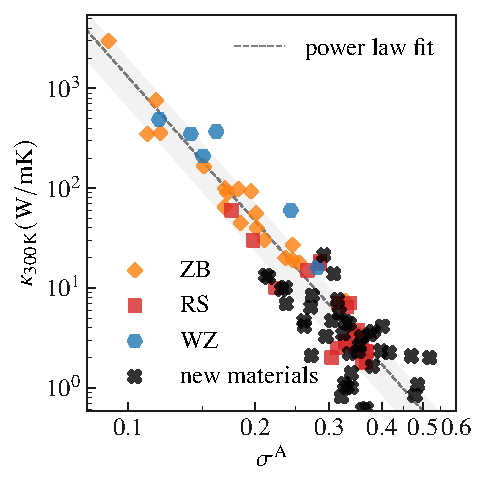
\includegraphics[width=\textwidth]{./data/plots/anharmonicity/9_kappa/incl_computations/sigma_vs_kappa_annot_comp_margin.pdf}
	\caption{
%	\mscomment{too crowded}
	Thermal conductivity at room temperature vs. anharmonicity measure. ZB: zincblende, RS: rock salt, WZ: wurtzite, cf. Fig.\,\ref{fig:anh.kappa}.}
	\label{fig:kappa_sigma_exp_comp}
\end{marginfigure}
%
\begin{marginfigure}
	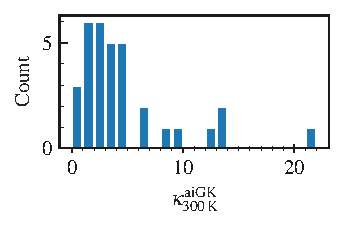
\includegraphics[width=\textwidth]{./data/plots/kappa_histogram/histogram.pdf}
	\caption{Summary of the range of thermal conductivities for materials without experimental reference found in this study.}
	\label{fig:kappa_wo_exp_hist}
\end{marginfigure}


\section{New materials and relation to anharmonicity}
\label{sec:results.new}
After validating the aiGK method against experimental literature, we present results for 33~materials \emph{without} experimental reference. We display these values in the context of the $\kappa$ vs. $\sigmaA$ plot introduced in Fig.\,\ref{fig:anh.kappa}, where we identified a power-law relation of experimental thermal conductivities with the anharmonicity measure $\sigmaA$ for simple elementary and binary materials. We show the data again in Fig.\,\ref{fig:kappa_sigma_exp_comp}, but this time including the additional, non-experimentally measured materials computed in this work.
%
It is apparent that the correlation between thermal conductivity $\kappa$ and $\sigmaA$ carries over from the simple materials to the more complex binary and ternary compound classes studied in this work, since the power-law fit in Fig.\,\ref{fig:kappa_sigma_exp_comp} is still performed with respect to the experimental values initially presented in Fig.\,\ref{fig:anh.kappa}. While the overall trend of decreasing thermal conductivity with increasing anharmonicity is clearly preserved, the spread of $\kappa$ values for materials with similar $\sigmaA$ or vice versa increases, which is expected due to the increased structural and chemical complexity of the studied materials.

Focusing on the new materials, we show a zoomed-in part of the $\kappa-\sigmaA$ plane in Fig.\,\ref{fig:kappa_sigma}, with only computational data, highlighting the materials where no experimental reference is available.
%
\begin{figure*}
	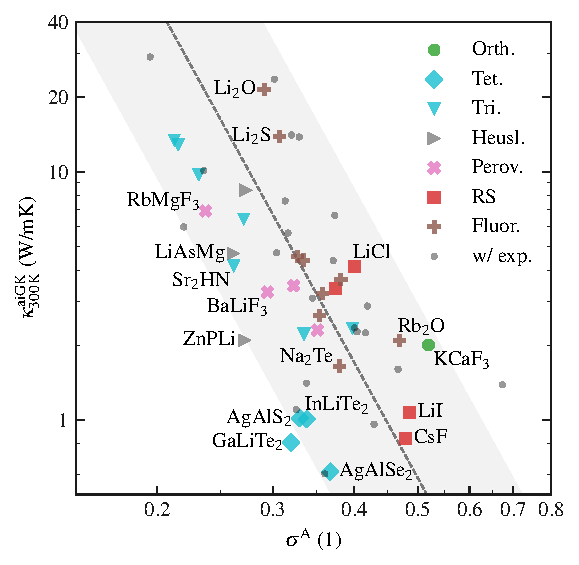
\includegraphics[width=.49\textwidth]{./data/plots/kappa_vs_sigma_trusted/kappa_vs_sigma_trusted.pdf}
	\hfill
	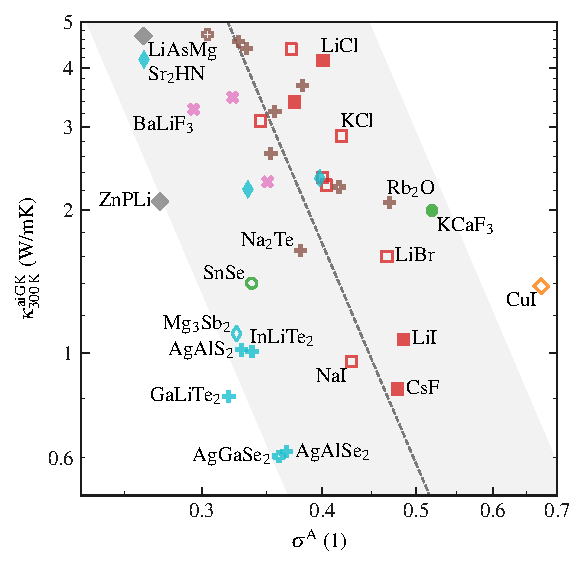
\includegraphics[width=.49\textwidth]{./data/plots/kappa_vs_sigma_trusted/kappa_vs_sigma_trusted_experiment_zoom.pdf}
	\caption{
	Thermal conductivity at room temperature computed via \emph{ab initio} Green Kubo (aiGK) vs. anharmonicity measure. Filled symbols denote materials without experimental reference. Left: Overview of studied materials without experimental reference. Materials with experimental reference are included as small dots for reference. Right: Zoom into the region $\kappa \leq 5$\,W/mK. Open symbols represent materials where experimental reference is available. The dashed line and shaded area are the same as in Fig.\,\ref{fig:kappa_sigma_exp_comp},~i.\,e.,~they represent a power-law fit to experimental thermal conductivities and a $\pm 50\,\%$ margin.}
	\label{fig:kappa_sigma}
\end{figure*}
%
In particular, we find 28 new materials with a computed bulk thermal conductivity of $\kappa^{\rm aiGK} < 10\,{\rm W/mK}$, 24 of which show $\kappa^{\rm aiGK} < 5\,{\rm W/mK}$, and 8 with $\kappa^{\rm aiGK} \leq 2\,{\rm W/mK}$,~i.\,e.,~comparable to the bulk thermal conductivity of existing and candidate thermoelectric materials such as Bi$_2$Te$_3$ and Bi$_2$Se$_3$ (1.3\,W/mK~\cite{Goldsmid.1956,Satterthwaite.1957}), PbTe (2.0\,W/mK~\cite{Elsharkawy.1983}), SnSe (1\,W/mK~\cite{Zhao.2014,Wei.2016,Sassi.2014}), M$_2$Sb$_3$ (2.3\,W/mK~\cite{Ahmadpour.2007,Pan.2020}), or GeTe (2.5\,W/mK~\cite{Perumal.2015}). A full list of all values is given in Tab.\,\ref{tab:kappa.noexp}, and a histogram of the values is shown in Fig.\,\ref{fig:kappa_wo_exp_hist}. The materials of very low thermal conductivity comprise simple binary, cubic materials such as the rock salt structures CsF ($\kappa^{\rm aiGK} = 0.84$) and LiI ($\kappa^{\rm aiGK} = 1.07$), or the fluorite structure Na$_2$Te ($\kappa^{\rm aiGK} = 1.64$), but also more complex structures such as the strongly anharmonic perovskites KCdF$_3$ ($\kappa^{\rm aiGK} = 1.67$) and KCaF$_3$ ($\kappa^{\rm aiGK} = 2.00$).


\subsection{Chalcopyrite systems}
\label{sec:chalcopyrites}
Particularly noteworthy is a class of ternary materials, so-called \emph{chalcopyrites}, a tetragonal crystal class closely related to the zincblende structure~\cite{Wasim.1979}. These crystals have been studied in the past primarily because of their non-linear optical properties~\cite{Ho.2014}, but also thermal transport properties have been studied~\cite{Spitzer.1970,Wasim.1979,Garbato.1979}, mainly because thermal transport can limit the optical efficiency in these devices~\cite{Beasley.1994}. However, experimental references for this class of materials are scarce, and do not agree well~\cite{Beasley.1994}. 
%
\begin{table}[ht]
  \centering
  \fontfamily{ppl}\selectfont
  \begin{tabulary}{\textwidth}{LC}
    \toprule
    Reference & Thermal conductivity at 300\,K (W/mK) \\
    \midrule
    Berger 1966 (experiment)~\cite{berger1969}   & $2.7$          \\
    Beasley 1995 (experiment)~\cite{Beasley.1994} & $1.1$          \\
    This work (theory)                           & $0.6 \pm 0.2$  \\
    \bottomrule
    \vspace{.5em}
  \end{tabulary}
  \caption{Overview of experimental references for AgGaSe$_2$.}
  \label{tab:exp.aggase2}
\end{table}
%
Picking AgGaSe$_2$ as an example, there are two distinct measurements available as summarized in Tab.\,\ref{tab:exp.aggase2}, ranging from $1.1-2.7$\,W/mK~\cite{Beasley.1994,berger1969}. These values are complemented by calculated values based on semi-empirical models, ranging from $4.8-9.0$\,W/mK~\cite{Wasim.1979,Rincon.1995}. Our computed thermal conductivities are collected in Tab.\,\ref{tab:exp.chalcopyrites}.
%
\begin{table}[ht]
  \centering
  \fontfamily{ppl}\selectfont
  \begin{tabularx}{\textwidth}{lXcXc}
    \toprule
    Material & & $\kappa^{\rm aiGK}$ (W/mK) & & $\sigmaA$ \\
    \midrule
	  AgAlS$_2$   & & $1.01 \pm 0.20$ & & 0.33 \\
          AgAlSe$_2$  & & $0.62 \pm 0.16$ & & 0.37 \\
          AgGaSe$_2$  & & $0.61 \pm 0.18$ & & 0.35 \\
          GaLiTe$_2$  & & $0.81 \pm 0.15$ & & 0.31 \\
          InLiTe$_2$  & & $1.01 \pm 0.26$ & & 0.33 \\
    \bottomrule
    \vspace{.5em}
  \end{tabularx}
  \caption{Overview of computed thermal conductivities for chalcopyrite materials.}
  \label{tab:exp.chalcopyrites}
\end{table}

Besides AgGaSe$_2$, there is experimental reference for the chemically closely related material, AgGaS$_2$, with a measured thermal conductivity of 1.4\,W/mK~\cite{Beasley.1994}.
%\footnote{While we included AgGaS$_2$ in our dataset, we needed to discard the material because of aiMD convergence problems. 
%\mscomment{what kind of problems?}
%However, we like to mention this material in the context of this study as potentially interesting material for future investigations.} 
While our computational data might underestimate the thermal conductivity in these compounds slightly\footnote{Please keep in mind, that the absolute errors are only of the order of 0.5-1\,W/mK.}, we nevertheless see a clear indiciation of very low intrinsic thermal conductivity in AgGaSe$_2$, and the chemically closely related compounds AgAlS$_2$ and AgAlSe$_2$. At least regarding their thermal transport properties, they are therefore comparable or even superior to the existing thermoelectric materials listed in the previous section, while being free of heavy metals such as Pb or Bi.
The class of chalcopyrite materials has recently been investigated in a high-throughput study conducted by Plata and coworkers~\cite{Plata.2021pre}. Their findings are overall in line with ours, supporting the finding that the class of chalcopyrite materials may comprise several promising thermal insulators.
 % Mg$_3$Sb$_2$~\cite{kajikawa2003,Condron.2006,Zhang.2009,Zhang.2018,Pan.2020,Ding.2021}.
%\todo{$\kappa_{\rm MgSb}^{\rm aiGK} = 1.10 \pm 0.26$}

To qualitatively elucidate the nuclear dynamics of the chalcopyrite systems, we present phonon spectral functions obtained from a temperature dependent model Hamiltonian for the nuclear system up to third-order displacements to estimate phonon-phonon interactions in Fig.\,\ref{fig:sqe_all}~\cite{Hellman.2013,Hellman.2013b,Squires}.
%
\begin{figure}
	\centering
	AgGaSe2$_2$ \hspace{3.7cm} AgAlSe$_2$\\
	% \includegraphics[width=0.49\textwidth]{./data/plots/spectral_functions/122.04.AgGaS2.12.png}
	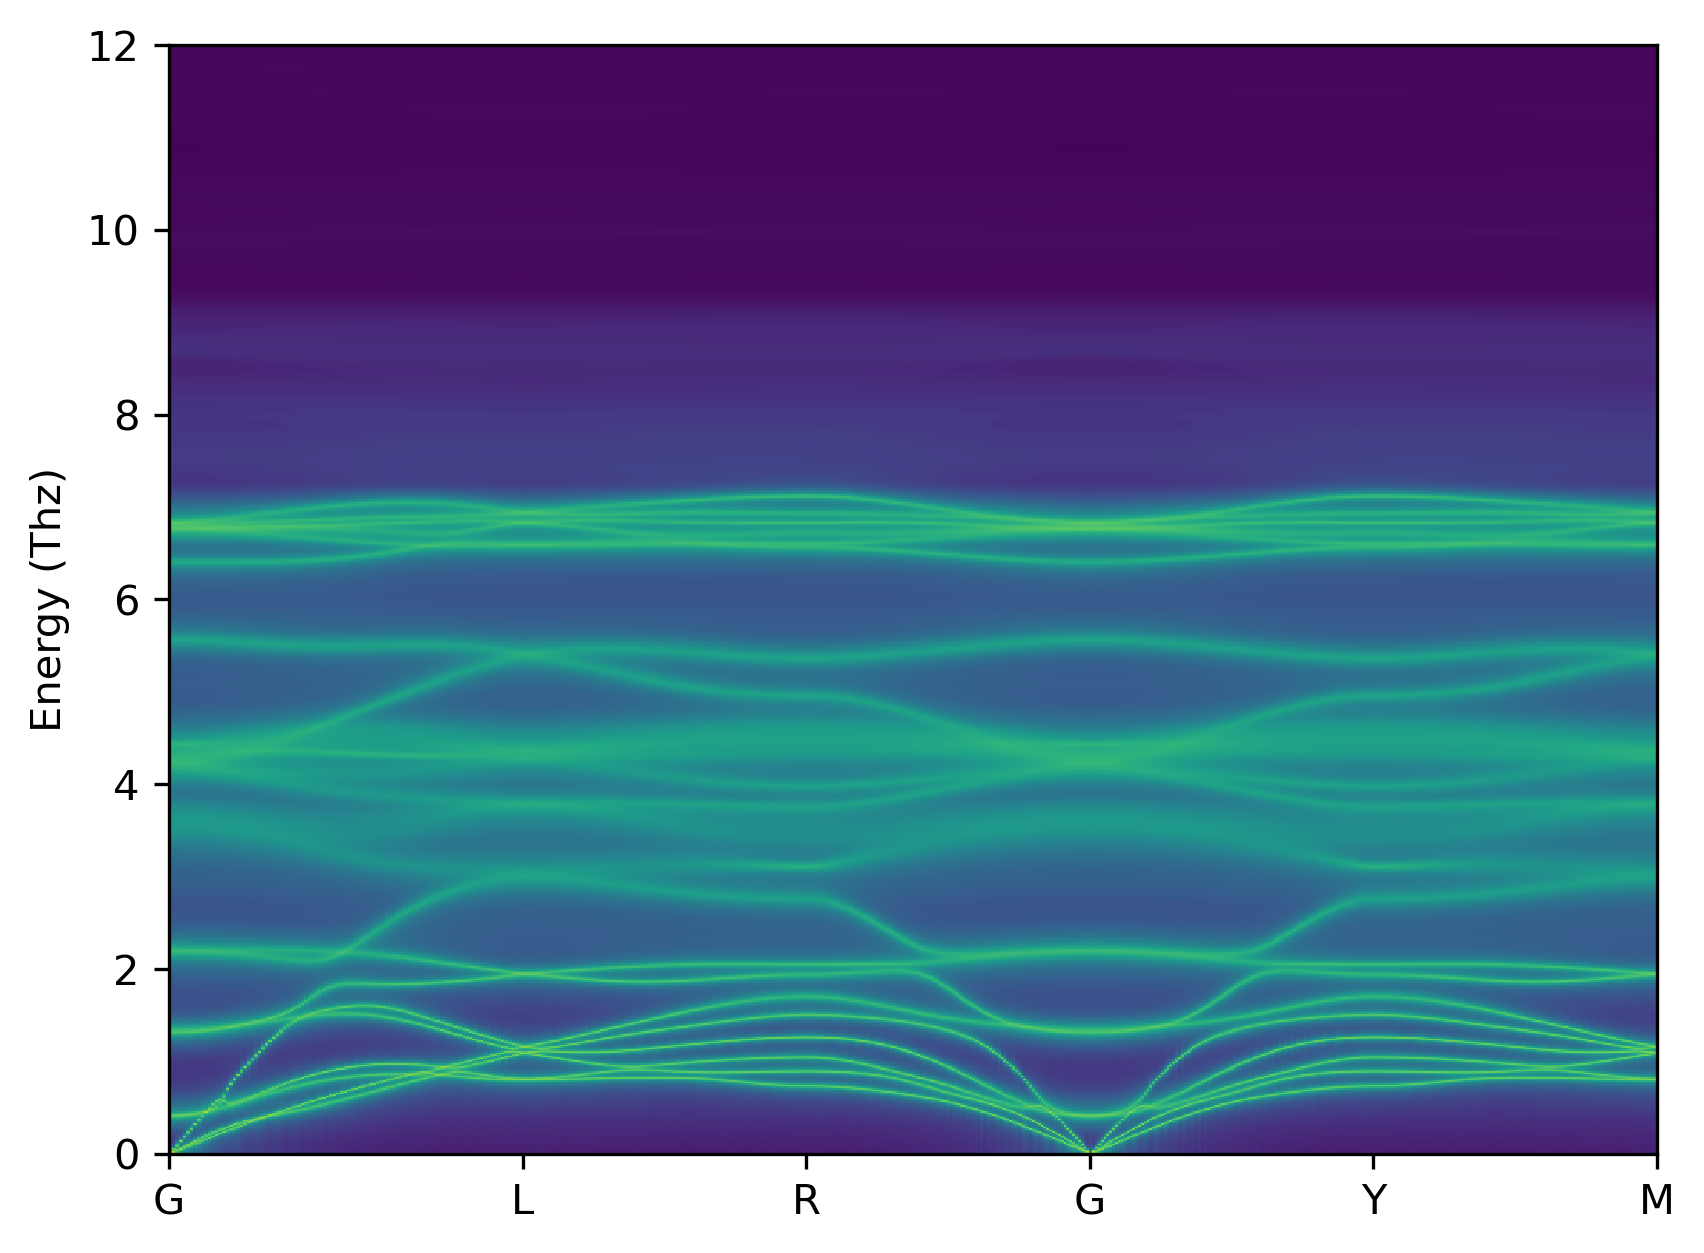
\includegraphics[width=0.49\textwidth]{./data/plots/spectral_functions/122.04.AgGaSe2.12.png}
	%	AgAlS$_2$ \hspace{3.7cm} AgAlSe$_2$\\
	%\includegraphics[width=0.49\textwidth]{./data/plots/spectral_functions/122.04.AgAlS2.15.png}
	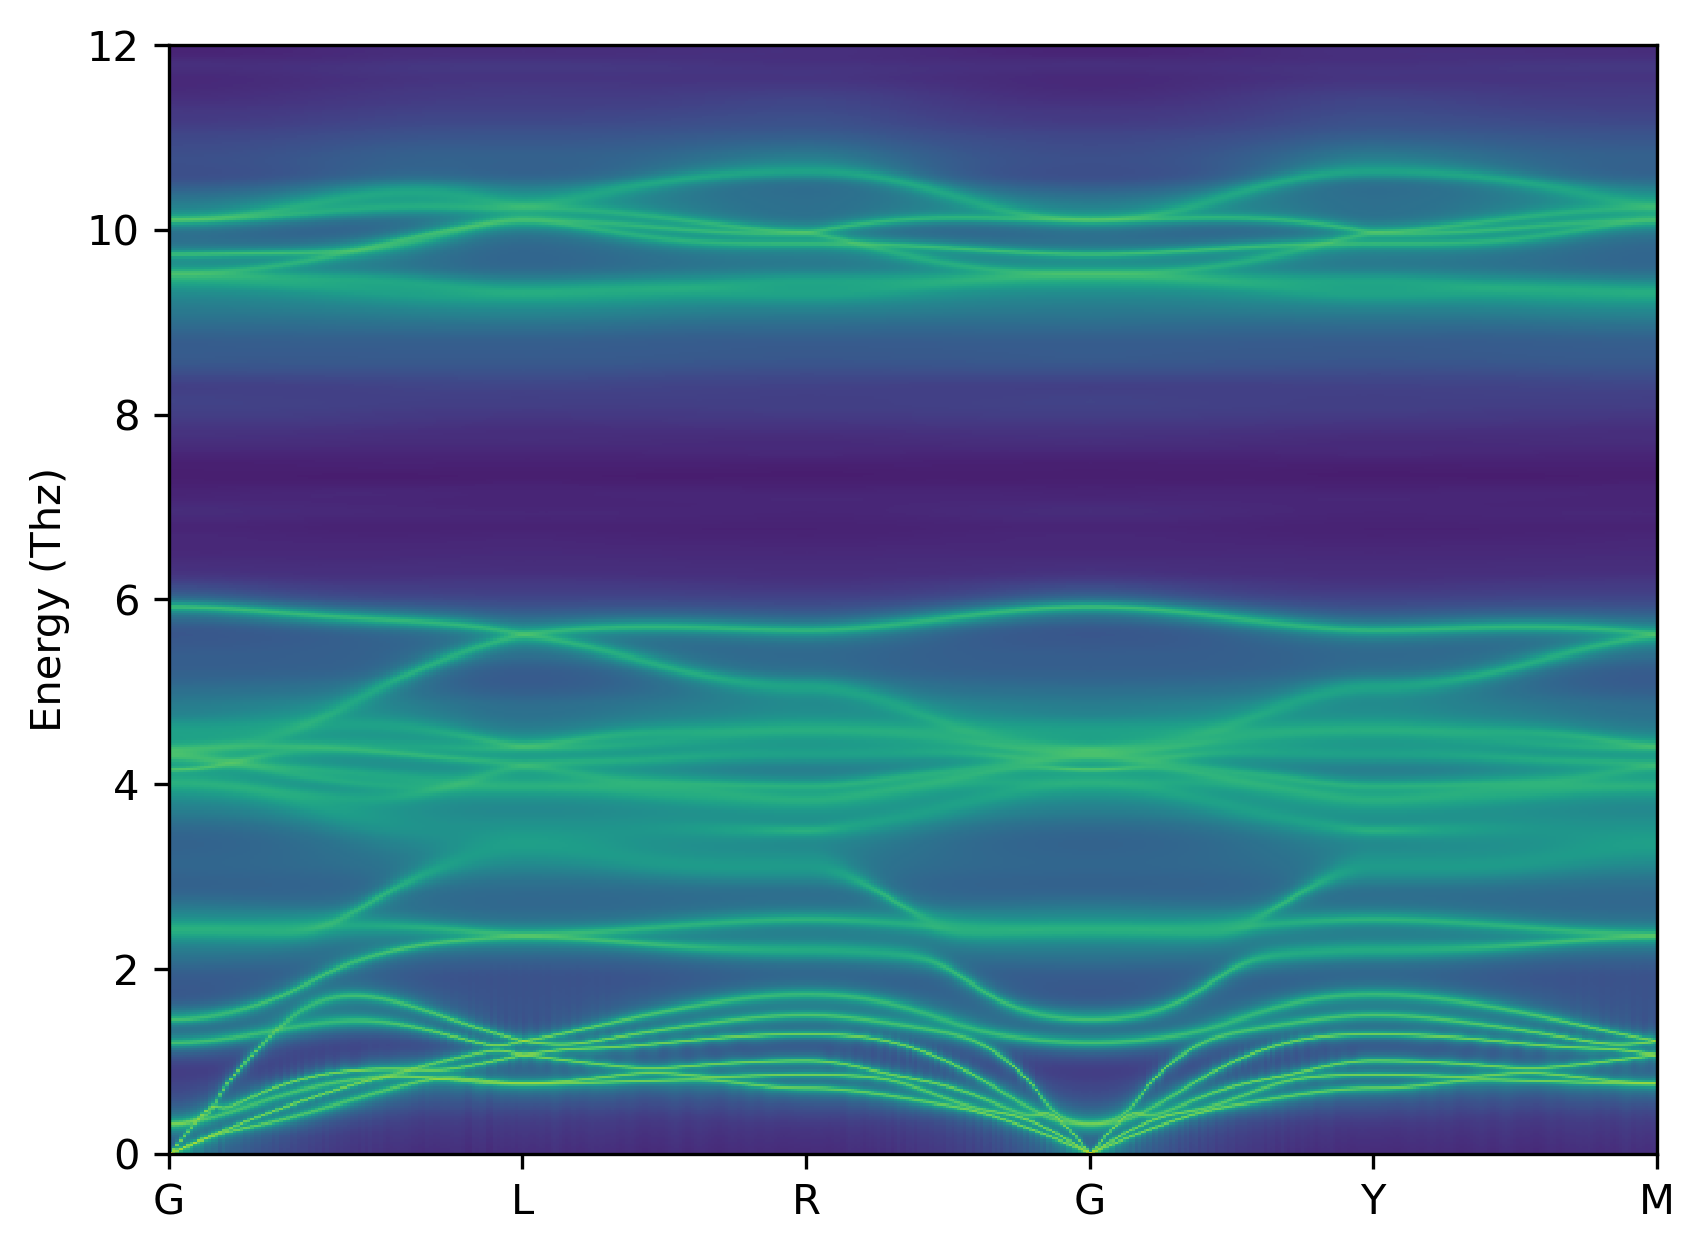
\includegraphics[width=0.49\textwidth]{./data/plots/spectral_functions/122.04.AgAlSe2.12.png}
	\\
	GaLiTe$_2$ \hspace{3.7cm} InLiTe$_2$\\
	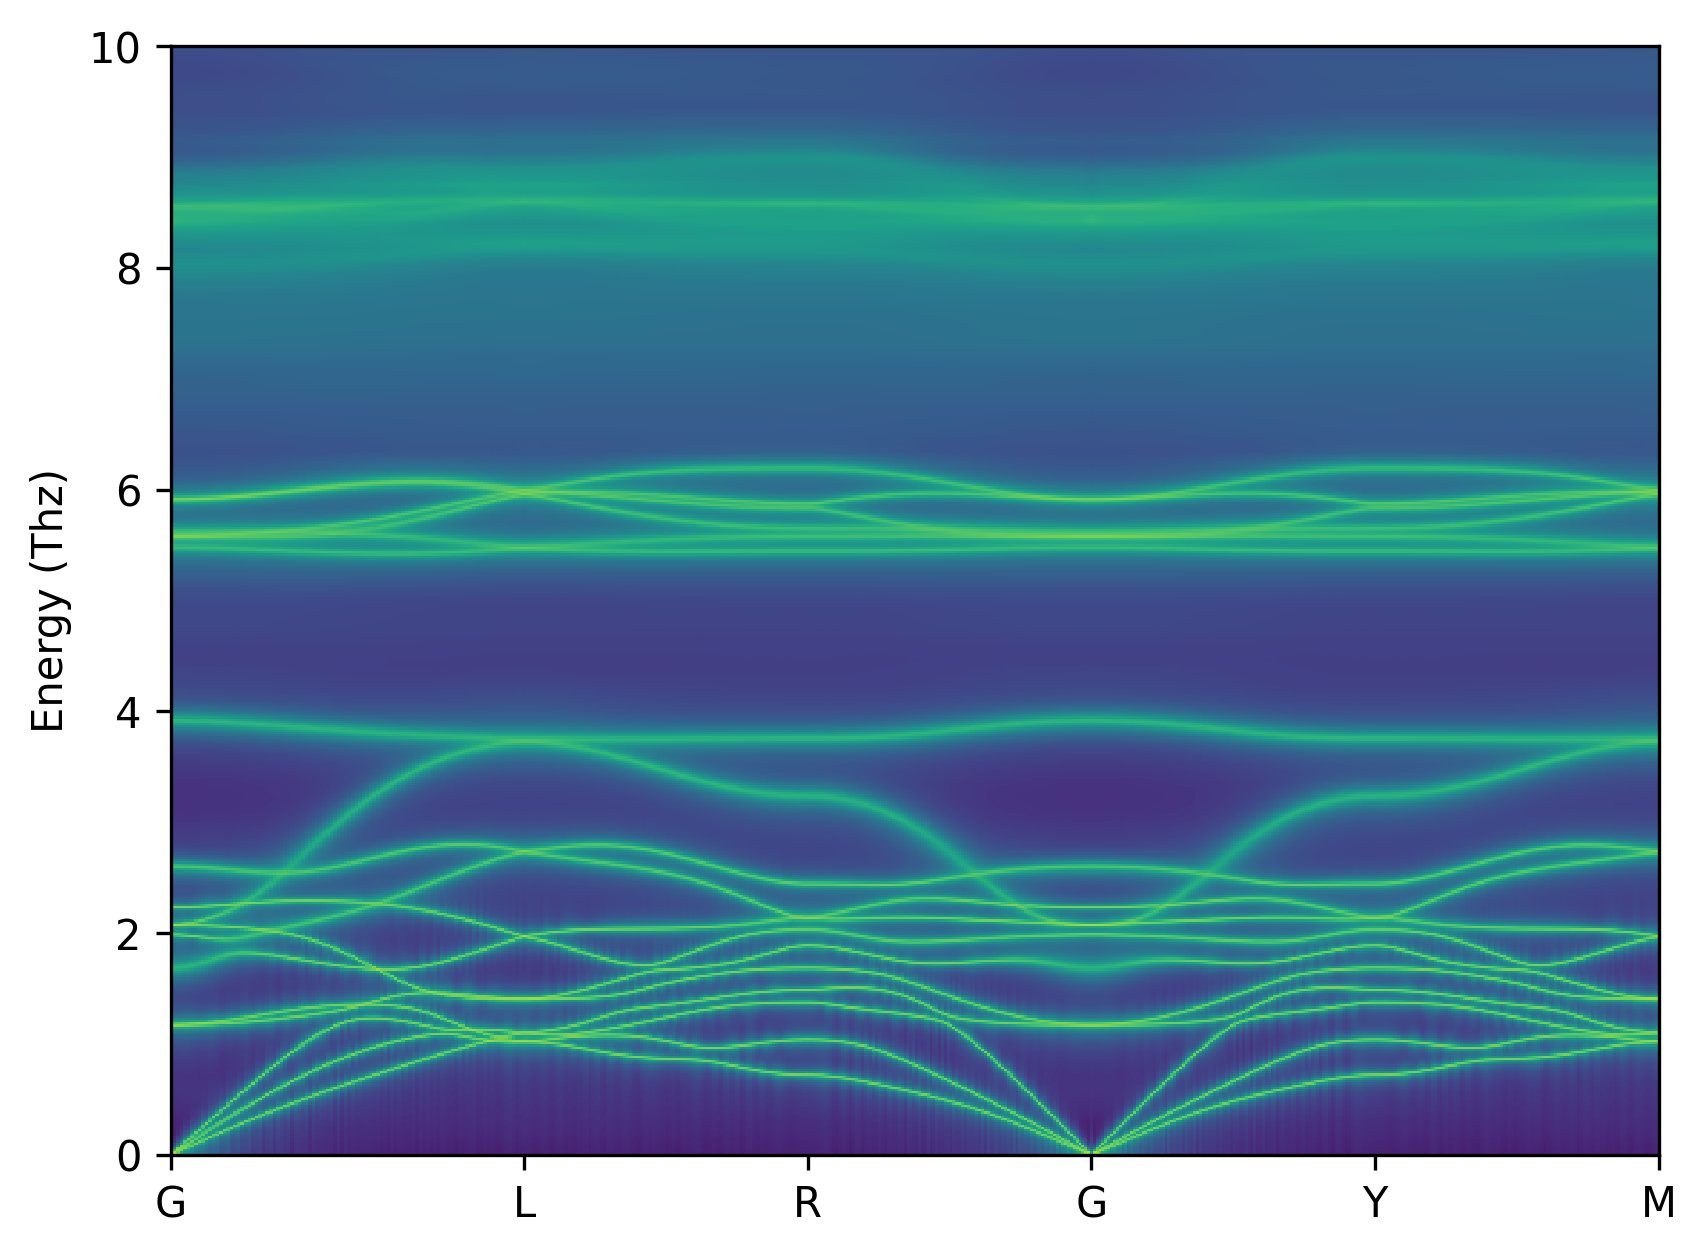
\includegraphics[width=0.49\textwidth]{./data/plots/spectral_functions/122.04.GaLiTe2.png}
	\includegraphics[width=0.49\textwidth]{./data/plots/spectral_functions/122.04.InLiTe2.png}
	\caption{Spectral functions for the chalcopyrite materials, AgGaSe$_2$, AgAlSe$_2$, GaLiTe$_2$, and InLiTe$_2$.}
	\label{fig:sqe_all}
\end{figure}
%
The common feature of these dispersions are the very flat acoustic branches which vary less than 1\,THz across the entire Brillouin zone, and a multitude of flat, nearly degenerate optical branches showing very litte to no dispersion. From a phonon-theory point of view, non-dispersive branches correspond to localized atomic motion in the system and therefore carry little heat beyond the Einstein-like diffusion of thermal energy from atom to atom, which is the dominant heat transport mechanism in structurally disordered systems like glasses~\cite{Simoncelli.2019}. Furthermore, in particular the optical branches are substantially broadened, which corresponds to strong anharmonic coupling in these systems, reducing their thermal conductivity.
%
\begin{table}[ht]
  \centering
  \fontfamily{ppl}\selectfont
\begin{tabularx}{\linewidth}{rXXX}
\toprule
Space group  &    material & $\kappa^{\rm aiGK}$ (W/mK) & $\sigmaA$  \\
\midrule
         122 & AgAlSe$_2$ &             0.62 &       0.37 \\
         122 & GaLiTe$_2$ &             0.81 &       0.32 \\
         225 &        CsF &             0.84 &       0.48 \\
         122 & InLiTe$_2$ &             1.01 &       0.34 \\
         122 &  AgAlS$_2$ &             1.01 &       0.33 \\
         225 &        LiI &             1.07 &       0.49 \\
         225 &   Na$_2$Te &             1.64 &       0.38 \\
          62 &   KCdF$_3$ &             1.67 &       0.53$^\dagger$ \\
          62 &   KCaF$_3$ &             2.00 &       0.52 \\
         225 &    Rb$_2$O &             2.08 &       0.47 \\
         216 &      ZnPLi &             2.09 &       0.27 \\
         166 & InNaSe$_2$ &             2.22 &       0.34 \\
         221 &  CsCdF$_3$ &             2.30 &       0.35 \\
         166 & InLiSe$_2$ &             2.34 &       0.40 \\
         225 &   Na$_2$Se &             2.63 &       0.35 \\
         225 &   Li$_2$Te &             3.24 &       0.36 \\
         221 &  BaLiF$_3$ &             3.27 &       0.29 \\
         225 &         KH &             3.39 &       0.37 \\
         221 &  RbZnF$_3$ &             3.47 &       0.32 \\
         225 &     K$_2$O &             3.67 &       0.38 \\
         225 &       LiCl &             4.14 &       0.40 \\
         166 &   Sr$_2$HN &             4.17 &       0.26 \\
         225 &    Na$_2$S &             4.40 &       0.33 \\
         225 &   Li$_2$Se &             4.55 &       0.33 \\
         216 &     LiAsMg &             4.67 &       0.26 \\
         166 &  LiScS$_2$ &             6.42 &       0.27 \\
         221 &  RbMgF$_3$ &             6.94 &       0.24 \\
         216 &      LiNZn &             8.42 &       0.27 \\
         166 &  InNaO$_2$ &             9.71 &       0.23 \\
         166 &  CuGaO$_2$ &            12.82 &       0.22 \\
         166 &  LiRhO$_2$ &            13.37 &       0.21 \\
         225 &    Li$_2$S &            13.85 &       0.31 \\
         225 &    Li$_2$O &            21.39 &       0.29 \\
\bottomrule
\end{tabularx}
  \caption{Bulk thermal conductivities for materials without experimental reference. $\dagger$: The anharmonicity measure for KCaF$_3$ is increased when the entire simulation is taken into account with $\sigmaA \approx 1.32$, since the simulation is close to a structural phase transition. We observe jumps in $\sigmaA (t)$ similar to those discussed for KCaF$_3$ in Sec.\,\ref{chp:anharmonicity}, but more pronounced. When KCdF$_3$ is close to the orthorombic reference, $\sigmaA \approx 0.53$. Structural phase transition are known to occur in KCdF$_3$ at around 470\,K~\cite{Hidaka.1977,Hidaka.1990}.}
  \label{tab:kappa.noexp}
\end{table}

\section{Conclusion}
We have estimated the convergence of aiGK simulations in terms of an effective simulation time focusing on the slow degrees of freedom of the system, and validated the approach against experimental values from the literature. In total, we computed thermal conductivities for 57 materials and verified our screening approach in terms of the anharmonicity measure $\sigmaA$. We found that the overall trend of decreasing thermal conductivity when anharmonicity increases initially inferred from the set of simple compounds carried over qualitatively to the more complex bulk materials considered in this work. We presented thermal conductivities for 33 materials where experiemental reference is not yet available, and identified the family of chalcopyrite crystals as a potentially interesting class of low thermal conductivity compounds, with several systems showing very low thermal conductivity of $\kappa \approx 1$\,W/mK at room temperature, which is comparable to or even below currently investigated thermoelectric candidates such as SnSe or Mg$_2$Sb$_3$~\cite{Zhao.2014,Wei.2016,Sassi.2014,Pan.2020,kajikawa2003,Condron.2006,Zhang.2009,Zhang.2018,Ding.2021}

%\mscomment{Limits should be discussed before results part.}
%\FK{So far the structure was i) Implementation (what do we do), ii) benchmark (how do we perform, what do we miss), iii) application (what do we find, knowing about possible shortcomings).}



% % \addtocontents{toc}{\protect\setcounter{tocdepth}{0}}
% % \addcontentsline{toc}{chapter}{Conclusion}
% \chapter{Conclusion}
% \section{Summary}

We have presented a systematic study of \emph{ab initio} thermal transport in experimentally known semiconductors and insulators, focusing on strongly anharmonic systems. To this end, we have developed a novel scheme based on first-principles force calculations which enables to measure the ``strength of anharmonicity'' in materials across chemical space, and facilitates to uncover strongly anharmonic dynamical effects in individual systems in a computationally efficient way~\cite{Knoop2020}. We found that this measure of anharmonicty,~$\sigmaA$,~correlates significantly with experimental thermal conductivities, and used the logic to predict materials with potentially low thermal conducitivity based on estimating their anharmonic strength.

To study heat transport in these systems, we have presented a comprehensive exposition of classical Green-Kubo theory from first principles in the framework of DFT, and discussed the implementation of a slightly adapted version of the \emph{ab initio} Green Kubo (aiGK) method first presented by Carbogno and coworkers in Ref.~\cite{Carbogno2016} in FHI-vibes~\cite{FHI-vibes}. In Chp.~\ref{sec:results.experiments}, we have verified this approach by computing thermal conductivities at room temperature for \CHECK 20~materials which are well characterized by experiments. We computed \todo{check} 37 more materials without experimental reference, finding \todo{check} 28 materials with low thermal conductivity $\kappa < 10$\,W/mK, with several materials in the range of state-of-the-art thermoelectrics $\leq 2$\,W/mK, in particular the class of chalcopyrite materials discussed in Sec.\,\ref{sec:chalcopyrites}.

The number of materials studied in this work with fully non-perturbative \emph{ab initio} Green Kubo theory of thermal transport is therefore an order of magnitude higher than all previously published results for solid systems combined. These comprise solid silicon and zirconia~\cite{Carbogno2016}, ice X~\cite{Grasselli2020}, and amorphous silica~\cite{Marcolongo2020}.\footnote{Further aiGK calculations have been published for liquids: Liquid Argon, heavy water, and water in different phases~\cite{Marcolongo2016,Marcolongo2020,Grasselli2020}.}

\newthought{From a methodological point of view}, we have presented a prototypical implementation of a data-driven approach for novel materials discovery: We leveraged existing knowledge to identify trends in material space based on an efficient descriptor, predicted candidate materials based on the descriptor, and studied the reduced number of materials by a high-accuracy method.

%\begin{itemize}
%	\item comprehensive exposition of (classical) GK theory from first principles in the framework of DFT
%	\item development of descriptor for identification of strongly anharmonic solids and effects~\cite{Knoop2020}
%	\item general implementation of aiGK method~\cite{Carbogno2016} in FHI-vibes~\cite{FHI-vibes}
%	\item aiGK results for XX materials
%		\subitem prediction of XX thermal conductivities in materials where no experiments were available before
%	\item prototypical implementation of a data-driven approach for novel material discovery
%		\subitem leverage experimental knowledge to identify trends in material space based on efficient descriptor
%		\subitem predict candidate materials based on descriptor
%		\subitem verify candidates by high-accuracy method
%\end{itemize}

\section{Outlook}
To conclude the thesis, we want to give a short outlook on topics and questions that naturally arise from this project.


\subsection{Remaining open questions}
\label{sec:outlook.open_questions}
One question that is not fully answered after this project is at which degree of anharmonicity fully non-perturbative Green Kubo calculations become necessary to compute accurate thermal conductivities, and when perturbative treatment in terms of cubic or cubic and quartic anharmonic contributions in the framework of self-consistent or effective phonons is sufficient~\cite{Hellman2013b,Feng2016,Tadano2018,Xia2018,Ravichandran2018}. The conceptual tools for studying this question have been laid out completely in this work: The anharmonicity measure~$\sigmaA$ can be generalized to quantify third, fourth, and higher order anharmonicity separately in straightforward manner. Furthermore, the molecular dynamics data produced in this work are made accessible to the community so that force constants models as input for perturbative expressions of thermal conductivity can be extracted with regression or sensing approaches~\cite{Zhou2014,Fransson2020}. And of course, the thermal conductivities computed in this work can serve as benchmark for identifying materials with significant deviations which are suited for further testing. This should be possible as of now at least for the binary systems with high symmetry studied in this work, as for more complex systems a treatment of quartic anharmonicity might become infeasible because of the unfavorite scaling of quartic force constants with number of irreducible atoms, see the discussion in appendix D of Ref.~\cite{Ravichandran2018}.

\subsection{Next steps for materials discovery}
Our screening for thermal insulators was governed by a single computational parameter,~i.\,e.,~the anharmonicity measure~$\sigmaA$. It is certain that including further structural and harmonic material properties in semi-empirical equations derived by feature extraction techniques can improve thermal conductivity predictions and thereby accelerate materials discovery~\cite{ouyang2018,goldsmith2017,Chen2019,Purcell2021}. The systematic data computed in the course of this project can serve as a testbed for these approaches.

\subsection{Next steps for ab initio Green Kubo}
As presented in the previous chapters, the \emph{ab initio} Green Kubo method in its current formulation uses an interpolation approach to deal with long-wavelength phonons, assuming an approximative scaling $\tau_{\b q, b} \propto \omega^{-2}_{\b q, b}$, where $\tau_{\b q, b}$ denotes the lifetime and $\omega_{\b q, b}$ the angular frequency of a phonon with wave vector $\b q$ and band index $b$. This relationship, however, only holds for crystals of certain lattice types in the limit of vanishing wave vector and small anharmonicity~\cite{Herring1954}. Especially when working on intermediate levels of anharmonicity, where phonons with long wavelengths are more important, an improvement of the current interpolation scheme is certainly desirable,~e.\,g.,~by using the full phonon spectral function $S(\b q, \omega)$ which implicitly contains information about frequencies $\omega_{\b q, b}$ and lifetimes $\tau_{\b q, b}$, lends itself for interpolation in momentum space, and can be systematically improved by surrogate models beyond the harmonic approximation~\cite{Maradudin1962}. More advanced surrogate models could also help to map out long-lived contributions better, thereby reducing the necessary amount of effective simulation time, $\teff$, by converging out the harmonic contribution to heat transport faster than in the current approach. The data produced in the course of this work can serve as a basis to develop and test ideas in that regard.


\subsection{Challenges for ab initio Green Kubo}
We see the following challenges with the current formulation of the \emph{ab initio} Green Kubo method that are worth further investigation: 

\newthought{The issues of defects and isotope scattering} have only been briefly mentioned in the discussion of thermal transport in MgO in Sec.~\ref{sec:mgo.experiments}, but have not been further investigated in this work, although they are known to impact thermal conductivity in actual materials~\cite{Bisson2000}. In a supercell-based \emph{ab initio} approach, these effects are notoriously difficult to study because of the required system sizes and time scales~\cite{Gibbons2011}. However, these are technical and not conceptual issues which might be possible to solve by the increasing computational power, or by surrogate models based on a DFT description of the potential energy surface, see also Sec.\,\ref{sec:outlook.ml}.

\newthought{The topic of convective contributions to the heat flux} has been touched in Chp.~\ref{chp:heat_transport}. As these are absent in the virial-based heat flux formulation used in this work, this rules out any study of materials with noticeable self diffusion. Furthermore, as discussed in Sec.~2.3.1 and appendix A of Ref.~\cite{ErcoleThesis}, there is no rigorous mathematical proof for the assumption of vanishing convective contributions to the thermal conductivity even in system without any self diffusion, since those can, in principle, contribute through the cross-correlation of convective and non-convective currents. While those are often negligible~\cite{Vogelsang1987}, it would be interesting to estimate the strength of this effect. One could compute convective contributions to the heat flux based on a force constants model, and evaluate its contribution. This should be sufficient to quantify the expected deviation, and materials with noticeable deviation could be interesting to study further, if any are found.

\newthought{Nuclear quantum effects (NQE)} have been mentioned in the discussion of LiF in Sec.\,\ref{sec:results.experiments}. These are inherently absent in the formulation of classical Green Kubo theory, and correct treatment of NQE for dynamical effects such as heat transport poses a formidable challenge already on a conceptual level,~i.\,e.,~in the defintion of a heat flux estimator, and the correct evaluation of Kubo-transformed quantum mechanical correlation functions. However, some very recent path-integral molecular dynamics based approaches using classical force fields show some promising progress in the field~\cite{Luo2020,Sutherland2021}.

\section{Perspective}
After discussing the status quo and potential futures of the methods used in this work, I want to discuss more long-term trends that are currently emerging in the field of heat transport simulations, and might have the power to push the topic forward considerably:
%In light of the constant development of solid state physics, materials science, and computational sciences, we see two main routes for the further improvement of the status quo in \emph{ab initio} heat transport simulations from equilibrium approaches: 
Green-Kubo simulations using machine-learned expressions for the potential energy function $\mathcal{V} ({\bf R})$~\cite{Korotaev2019,Li2020,Mangold2020}, and model Hamiltonian-based approaches using Boltzmann transport theory~\cite{Simoncelli2019} or analytical Green's functions~\cite{Isaeva2019,dangic2021}.

\subsection{Machine learning Green Krubo}
\label{sec:outlook.ml}
The advent of machine-learned potentials with \emph{ab initio} quality~\cite{Lorenz2004,Behler2007,Bartok2010,Bartok2013,shapeev2016} coupled with on-the-fly or active-learning training strategies~\cite{Li2015,Jinnouchi2019,podryabinkin2017,Liu2021} promises to become a versatile tool for dynamical simulations of materials in a range of subfields, especially for phenomena where the electronic structure of a given material is only of secondary importance,~i.\,e.,~in uncharged systems with electronically trivial defects. In such materials, machine-learned potentials can remove computational bottlenecks when aiming for statistical convergence in simulation time, as well as system and ensemble sizes, which in turn could make GK-based transport simulations of new materials accessible to more researchers than currently.

While several proofs of principle for GK simulations from machine-learned potentials exist already~\cite{Korotaev2019,Li2020,Mangold2020}, some more fundamental problems persist,~e.\,g.,~the question of transferability across temperature and phase transitions in particular, or how long-range electrostatic interactions in polar systems can be properly described in these models~\cite{Artrith2011,Grisafi2019,yue2021,kovacs2021}. From materials discovery perspective, where one aims at studying a multitude of systems, it remains to be seen how straightforward and robust the parametrization of these force fields can be achieved in practice, and if the extra cost in human time in order to train the potentials can be reduced to a minimum without compromising their reliability. The aiGK data computed and made available in the course of this project can help to develop and benchmark these approaches.


\subsection{Boltzmann transport and analytical Green's functions}
A complementary route for not too complex materials is the use of model Hamiltonians coupled with perturbation theory in the framework of lattice dynamics, which become increasingly sophisticated and continue to develop~\cite{Esfarjani2008,Hellman2013,Hellman2013b,errea2014,Tadano2018,Zhou2019}. While these approaches are limited to non-diffusing materials with a definite long-range structural order and limited complexity,\footnote{See comments in Sec.\,\ref{sec:outlook.open_questions}.} they allow to study subtle dynamical effects such as the the behavior of thermal transport close to and across phase transitions with very good precision~\cite{dangic2021}, which is particularly important for potential thermoelectrics such as SnSe and GeTe~\cite{zhao2014,Dewandre2016,dangic2021}. Further, these methods give straightforward access to nuclear quantum effects~\cite{shulumba2017}, which is a formidable task for molecular dynamics-based Green Kubo methods as discussed above.

Worth noting are more recent approaches that try to bridge the gap between state of the art Boltzmann transport~\cite{Simoncelli2019} and analytical Green Kubo in terms of phonon Green's functions~\cite{Isaeva2019,dangic2021}. Combined with self-consistent sampling techniques~\cite{brown2013}, these approaches promise to be a very efficient alternative for heat transport simulations in a wide class of solid systems.

Last but not least, lattice-dynamics techniques can be coupled with molecular dynamics simulations to extract fully anharmonic properties such as phonon lifetimes,~e.\,g.,~as we use them in the \emph{ab initio} Green Kubo method~\cite{Ladd1986,Turney2009,Zhang2014,Carbogno2016,Glensk2019} -- the opportunities for combining these approaches are certainly not exhausted.



%\subsection{Exascale computing}
%We don't expect any novel physics being discovered through exascale computing.

%\subsection{Novel physics}
%At last, we would like to remark a few things about challenges from a physicist's point of view.
%
%\begin{itemize}
%	\item Methods:
%		\subitem ML potentials to make GK more feasible and accessible, remove computational bottleneck, go beyond GGA accuracy  
%		potentials:
%		\cite{Behler2007,Bartok2010,Bartok2013,shapeev2016}
%		long-range:
%		\cite{Artrith2011,Grisafi2019,yue2021,kovacs2021}
%		active learning/on the fly:
%		\cite{Li2015,Jinnouchi2019,podryabinkin2017,Liu2021}
%  	Shapeev: \cite{Korotaev2019},	DeepotSE: \cite{Li2020}, DonadioBehler: \cite{Mangold2020}
%		\subitem analytical GK: crossover between GK and BTE approach for not-too-complex materials
%		\cite{dangic2021,Simoncelli2019,Isaeva2019}
%			\subsubitem NQE? \cite{shulumba2017,sutherland2021}
%		\subitem Question of reference positions, esp. close to phase transitions. Time-dependent?
%		\subitem 2D structures: People just do 3D transport, nobody really knows what's going on in 2D
%		\subitem Magnetism: No real theory for thermal transport in magnetic materials, only ad-hoc explanations like \cite{stockem2018}.
%		\subitem More generally: difficult systems for DFT, can be as banal as band-gap closing as observed for ZnSb
%	\item materials discovery
%		\subitem highlight that $\sigmaA$ is able to describe main trend in material space, improving on that by including more descriptors very well possible, will enable to accelerate novel materials discovery for thermal insulators
%			\CITE{Purcell?,Ramprasad,SISSO,Subgroup discovery,...}
%			\cite{ouyang2018,goldsmith2017,Chen2019}
%		
%		\subitem Screening depends crucially on the choice of the screened materials,~i.\,e.,~materials not included in the screening cannot be found.
%		
%		\subitem only bulk systems considered \cite{ferrando2020}
%\end{itemize}

\cleardoublepage
\phantomsection
\addcontentsline{toc}{chapter}{Bibliography}

\bibliographystyle{unsrt}
\bibliography{references,references_experiments}

% \setcounter{secnumdepth}{-1}

\part*{Appendix}

% \setcounter{tocdepth}{1}
% \addtocontents{toc}{\setcounter{tocdepth}{0}}
\addtocontents{toc}{\protect\setcounter{tocdepth}{0}}
\newcommand{\bibsection}{\section{Bibliography}} % <- was missing

\begin{appendices}
%  \appendixpage
  \part*{Appendix}
  \chapter{Bloch Theorem and Brillouin Zone}
\epigraph{\singlespacing \it ``The idea of periodicity in the reciprocal space is useless but, I think, harmless.''}{Paul Gartner}
\section{Bloch Theorem}
\label{sec:BlochTheorem}
The Schr\"odinger equation in 1d reads
\begin{align}
	\hat H \psi (x) = \left( - \frac{\nabla^2}{2m} + V(x) \right) \psi (x) = E \psi (x)~.
	\label{eq:app.bloch.se}
\end{align}
In a periodic potential,
\begin{align}
	V(x + a) = V(x)~,
	\label{eq:app.bloch.potential}
\end{align}
the periodicity can be expressed by stating that the translation operator $\hat T_a$ defined by its action,
\begin{align}
	\hat T_a f(x) = f(x + a)~,
	\label{eq:app.bloch.Ta}
\end{align}
commutes with the Hamiltonian,
\begin{align}
	\left[ \hat H , \hat T_a\right] = 0~.
	\label{eq:app.bloch.commute}
\end{align}
The eigenstates $\psi (x)$ of $\hat H$ are therefore also eigenstates of $\hat T_a$~\cite{Basdevant2000}. The translation operator is unitary, $\D{\hat T}_a = \hat{T}_a^{-1}$, but not hermitian. The eigenvalues $\lambda$ associated with $\hat T_a$ are thus complex numbers. By definition, one has \mbox{$\psi ( x + na ) = \lambda^n \psi(x)$}. Requiring bounded solutions, $\lim_{x \rightarrow \infty} \lvert \psi (x) \rvert < \infty$, imposes the condition $\lvert \lambda \rvert = 1$.
The function $\psi$ can therefore be written as
\begin{align}
	\psi (x) = c(x) u(x)~,
\end{align}
with a real, periodic function
\begin{align}
	u: \mathds R \rightarrow \mathds R
	\quad\text{with}\quad u(x + a) = u(x)~,
\end{align}
and a complex function of unit modulus,
\begin{align}
	c: \mathds R \rightarrow \mathds C
	\quad\text{with}\quad \left\lvert c(x) \right\rvert = 1~.
	\label{eq:app.bloch.c1}
\end{align}
We label each possible solution by the number $k$, then
\begin{align}
	c_k (x) = {\rm e}^{\im k x}
	%% don't impose uniqeness here
	%\quad\text{with}\quad k \in \left[0, \frac{2 \pi}{a} \right)
	\label{eq:app.bloch.c2}
\end{align}
% is a unique map from the domain $x \in [0, a)$ to the complex unit circle $\set{z \in \mathds C : \lvert z \rvert = 1}$. 
is a map from the domain $x \in \mathds R$ to the complex unit circle $\set{z \in \mathds C : \lvert z \rvert = 1}$. 
It then holds that $\hat T_a \psi_k (x) = {\rm e}^{\im k a} \psi(x)$,~i.\,e.,~$\psi_k$ is an eigenfunction of $\hat T_a$ with eigenvalue $\lambda = {\rm e}^{\im k a}$. We formulate the
\begin{thm}[Bloch]
	Solutions to the Schr\"odinger equation~\eqref{eq:app.bloch.se} with a periodic potential of periodicity $a$ are of the form
	\begin{align*}
		\psi_k (x) = {\rm e}^{\im k x} u_k (x)~,
	\end{align*}
	with a real, periodic function $u_k$.
%	 for each $k$ in the first Brillouin zone,
%	\begin{align*}
%		k \in \left[0, \frac{2 \pi}{a} \right)~.
%	\end{align*}
\end{thm}
The theorem is trivially extended to the 3d case by using the multiplication rule
\begin{align}
	\hat{T}_{{\bf a} + {\bf b}} f({\bf x}) = \hat{T}_{\bf a} \hat{T}_{\bf b} f({\bf x}) \equiv f({\bf x} + {\bf a} + {\bf b})~.
\end{align}
A more rigorous proof in terms of representation theory can be found,~e.\,g.,~in~\cite{Dresselhaus2007}.

\section{Brillouin Zone}
\label{sec:BrillouinZone}
We have not yet specified the range of the quantum number $k$. This can be done by requiring the complex function $c_k$ defined in Eq.\,\eqref{eq:app.bloch.c2} to map the interval $x \in [0, a)$ \emph{exactly once} to the unit circle so that $k$ is a \emph{unique} label for the eigenvalues ${\rm e}^{\im k a}$ of the translation operator $\hat T_a$.
We therefore define the
\begin{align}
	\text{Brillouin zone} = \set{k : k \in \left[ - \frac{\pi}{a}, \frac{\pi}{a}\right)}~.
\end{align}
For a wavefunction belonging to $k' = k + G$, where $G$ is an integer multiple of the the reciprocal lattice vector $b = 2\pi / a$, we would find
\begin{align}
	\hat T_a \psi_{k + G} (x) = {\rm e}^{\im k a} \psi_{k + G} (x)~.
\end{align}
They are therefore indistinguishable by the translation operator and we define $\psi_k$ and $\psi_{k+G}$ to be the same function,
\begin{align}
	\psi_k (x) = \psi_{k + G} (x)~.
\end{align}
This is sometimes termed ``periodicity of Bloch functions in reciprocal space''.

\chapter{Born-von Karman Supercell}
To ensure normalizability of the functions $\psi_{{\bf k}l}$, one additionally imposes the \emph{Born-von Karman boundary conditions}
\begin{align}
\psi_{{\bf k}l} ({\bf x} + {\bf A}_i) 
= \psi_{{\bf k}l} ({\bf x})
%\label{eq:dft.Bloch.4}
\end{align}
where each ${\bf A}_i$ is a linear combination of the primitive basis vectors $\set{{\bf a}_i}$,
\begin{align}
{\bf A}_i = S_i^{~j} {\bf a}_j\quad\text{with } S_i^{~j} \in \mathds Z~,
\end{align}
where $S$ is a non-singular matrix with integer elements. The space spanned by the $\set{{\bf A}_i}$ is parallelepiped of volume $V = N \, {\bf a}_1 \cdot ({\bf a}_2 \times {\bf a}_3)$, where $N = \det S$ is the number of unit cells that fit into the enlarged cell. This cell is therefore often called \emph{supercell}, and the matrix $S$ is denoted as a \emph{supercell matrix}.
With the Born-von Karman boundary conditions, the domain of all functions and functionals appearing in the Kohn-Sham equations become restricted to the supercell. The ideal, infinite crystal is obtained in the limit $N \rightarrow \infty$.
Using the periodic boundary condition expressed by Eq.\,\eqref{eq:dft.Bloch.4} in the Bloch functions given by Eq.\,\eqref{eq:dft.Bloch.2}, and the periodicity of the functions $u_{{\bf k} l}$, one finds that
\begin{align}
%	{\rm e}^{\im {\bf k} \cdot ({\bf x} + N_i {\bf a}_i)} u_{{\bf k} l} ({\bf x})
%		&= {\rm e}^{\im {\bf k} \cdot {\bf x}} u_{{\bf k} l} ({\bf x}) \nonumber \\
%	\implies
%		{\rm e}^{\im {\bf k} \cdot  N_i {\bf a}_i} 
%			&= 1 \nonumber \\
%	\implies
{\bf k} \cdot {\bf A}_i
&= 2 \pi m_i\quad\text{with } m_i \in \mathds N \text{ such that } 
\forall i: {\bf k} \cdot {\bf a}_i \leq 2 \pi~.
%\label{eq:dft.Bloch.5}
\end{align}
In total there are $N$ permissible values of $\bf k$ labelled by ${\bf m} = (m_1, m_2, m_3)$ that can be expressed in terms of the \emph{reciprocal lattice vectors}~\cite{Sands2002}
\begin{align}
{\bf B}^i 
= 2 \pi \varepsilon^{ijk} \frac{{\bf A}_j \times {\bf A}_k}{{\bf A}_1 \cdot ({\bf A}_2 \times {\bf A}_3)} ~,
%\label{eq:dft.Bloch.bi}
\end{align}
where $\varepsilon^{ijk}$ denotes the Levi-Civita symbol enforcing the correct ordering of $ijk$. The complete set of $\bf k$-values is
\begin{align}
{\bf k}_{\bf m} 
= \sum_{i=1}^3 m_i {\bf B}^i~.
%\label{eq:dft.Bloch.k_m}
\end{align}
The values of $\bf k$ given by Eq.\,\eqref{eq:dft.Bloch.k_m} are those sampled in real-space simulation in a box of the given size,~i.\,e.,~the \emph{Born-von Karman cell}.

\chapter{Finite Differences Force Constants}
The force constants $\Phi$ can be obtained from first-order derivatives of the potential-energy surface,~i.\,e.,~the forces, by rewriting the second derivative in terms of a finite difference expression,
\begin{align}
\Phi_{I \alpha, J \beta}
= \left.\frac{\partial^{2} \mathcal{V}(\mathbf{R})}{\partial R_{I}^{\alpha} \partial R_{J}^{\beta}}\right|_{\mathbf{R}^{0}}
= - \frac{\partial}{\partial R_I^\alpha} F_{J, \beta}
= - \lim_{\epsilon \to 0}
\frac{F_{J, \beta} (\set{\b R': R^{\prime \alpha}_I = R^{0, \alpha}_I + \epsilon )}}{\epsilon}
~.
\label{eq:FC2_finite}
\end{align}
In practice, atom $I$ is displaced by a small but finite displacement $\epsilon$ in the direction $\alpha$, and the force on all other atoms is recorded. By performing the displacement in all $3N$ degrees of freedom, the $3N \times 3N$ forces can be arranged in a matrix ${\rm F}_{[3N \times 3N]}$, and the displacements can be arranged in a matrix ${\rm U}_{[3N \times 3N]} = \epsilon \mathds 1_{[3N \times 3N]}$. The $3N \times 3N$ force-constants matrix $\Phi$ is obtained by the trivial matrix multiplication
\begin{align}
{\rm F }
&= - \Phi {\rm U} 
= - \epsilon \Phi \mathds 1
\label{eq:finite.diff.1}
\\
\implies
\Phi &= - \frac{1}{\epsilon} {\rm F} \mathds 1~.
\end{align}
%\begin{align}
%	F &= - H U \\
%	\implies
%	H &= - U^{+} F \\
%	F &= \begin{pmatrix} \b F_1, & \cdots, & \b F_{3N} \end{pmatrix}
%\end{align}
If $M > 3N$ displacements are used,~e.\,g.,~because positive and negative displacements $\pm \epsilon$ are used, the force constants can be obtained by solving an overdetermined linear equation of the kind
\begin{align}
{\rm F}_{[3N \times M]} &= - \Phi_{[3N \times 3N]} {\rm U}_{[3N \times M]} \\
\implies
\Phi &= - {\rm F} {\rm U}^{+}~,
\label{eq:phi.pseudo.1}
\end{align}
where ${\rm U}^{+}$ denotes the Moore-Penrose pseudo inverse of the displacement matrix $\rm U$~\cite{Penrose1955,Parlinski1997}.

\newthought{The number of required force calculations} can be reduced by considering the spacegroup symmetry of the crystal. This can be achieved in two ways: First, the symmetry can be used to identify the set of inequivalent displacements from which all other forces can be constructed by the following argument: We define the representation $\Gamma^g$ of a symmetry operation $g$ by its action on the atomic coordinates $\set{\b R_I = \b R_I^0 + \b U_I}$ as
\begin{align}
\b R_I^{g} &\equiv {\Gamma}^g (\b R_I) = { P}^g_{IJ} \b R^0_J + { M}^g \b U_I~,
\label{eq:sym.RI'}
\end{align}	
where $P^g_{IJ}$ is the permutation that relates the reference positions of atom $I$ and atom $J$, and $M^g$ is an orthogonal matrix representing the rotation (or inversion) of the respective displacement. 
\begin{marginfigure}
	\centering
	\includegraphics[width=\textwidth]{./data/sketches/symop.jpg}
	\caption{The configurations $\b R$, $\b R^g$, and $\tilde{\b R}^g$ obtained from the symmetry operation $g=\text{90 degrees rotation}$ for a two-dimensional system with five atoms. Arrows indicate the force at each atom.}
	\label{fig:symmetry.1}
\end{marginfigure}
As depicted in Fig.~\ref{fig:symmetry.1}, the forces on each atom in the rotated system $\b R^g = \set{\b R^g_I}$ are obtained by co-rotating the forces in the initial configuration $\b R = \set{\b R_I}$ as
\begin{align}
\b F_I (\b R^g) &= {M}^g \b F_I (\b R)~,
\label{eq:sym.Fp}
\end{align}
i.\,e.,~the forces transform as the displacements $\b U_I$. Let us now define a new configuration $\tilde{\b R}^g$ where just the displacements $\b U_I$ are rotated according to $g$. This can be achieved by rotating the entire system according Eq.\,\eqref{eq:sym.RI'} and applying the inverse permutation $P^{g-1}$,~i.\,e.,
\begin{align}
\tilde{\b R}_I^g 
&= P^{g-1}_{IJ} \b R_I^g 
\stackrel{\eqref{eq:sym.RI'}}{=} \b R^0_I + {\rm M}^g P^{g-1}_{IJ} \b U_J~.
\end{align}
It follows that the force on atom $I$ in the new configuration $\tilde{\b R}^g$ is related to the force in the rotated system $\b R^g$ by this inverse permutation, so that
\begin{align}
\b F_I (\tilde{\b R}^g) 
&= {P}^{g-1}_{IJ} \b F_J (\b R^g) 
= {M}^g  {P}^{g-1}_{IJ} \b F_J (\b R)~.
\label{eq:sym.Ftilde}
\end{align}
By means of this equation, the set of forces obtained for a configuration $\set{\b R_I = \b R_I^0 + \b U_I}$ can be used to generate a set of forces for each symmetrically equivalent configuration $\set{\tilde{\b R}_I^g = \b R_I^0 + {\rm M}^g P^{g-1}_{IJ} \b U_J}$, where $g$ are spacegroup elements.

A complementary approach is to use the symmetry elements $\set{g}$ to reduce the forceconstant matrix to an irreducible basis,
\begin{align}
\Phi 
= \sum_{i=1}^{D} p_i \tilde{\Phi}_i~,
\label{eq:sym.Phi.irrep.1}
\end{align}
where the $\tilde{\Phi}_i$ are \emph{solely} determined by the space group elements $\set{g}$ and analytical properties of the forceconstants, and only the \emph{irreducible components} $p_i$ are system dependent. The pseudoinverse procedure given in Eq.\,\eqref{eq:phi.pseudo.1} then only has to be performed for the $D$ parameters $p_i$~\cite{Parlinski1997}. This procedure can drastically reduce the number of free parameters in the forceconstant matrix. For example, in a $4\times4\times4$ bcc lattice with 128 atoms, $\Phi$ is a matrix with $(3 \cdot 128)^2 = 147456$ elements. However, there are only $D=11$ irreducible parameters $p_i$ that need to be determined~\cite{Hellman2013}.

\TODO{Add the theory for symmetry reduction}

\chapter{Linear Response Distribution Function}
\label{app:lr.f}
To solve for $\Delta f(t)$ defined in Eq.\,\eqref{eq:lr.df.2}, we introduce a shorthand notation such that
\begin{align}
\frac{\d \Delta f}{\d t} = -\im L \Delta f(t) - \im \Delta L (t) f^0~,
\label{eq:lr.df.3}
\end{align}
where the Liouville operator $L^0$ is defined by
\begin{align}
	\im L^0 g = \set{g, H^0}~,
	\label{eq:app.lr.L}
\end{align}
and similarly
\begin{align}
	\im \Delta L (t) g = \set{g, H'(t)}~.
	\label{eq:app.lr.L'}
\end{align}
Equation~\eqref{eq:lr.df.3} is a first order linear differential equation of the form
\begin{align}
	\frac{\d y}{\d t} + p(t) y = q(t)~,
	\label{eq:app.lr.dgl.1}
\end{align}
which is straightforward to solve by using an integrating factor as follows: We identify $y = \Delta f$, $p(t) = \im L^0$, and $q(t) = - \im \Delta L (t) f^0$. Following Ref.~\cite[p.\,68]{Lomen1986}, we define the integrating factor \mbox{$\rho (t) = \exp(\int \d t \, p (t)) = \exp (\im L^0 t)$}, multiply Eq.\,\eqref{eq:lr.dgl.1} with $\rho (t)$, and use that \mbox{$\frac{\d}{\d t} \, \rho(t) = \rho(t) p(t)$} to obtain
$$
\frac{\d}{\d t} (\rho (t) y) = \rho(t) q(t)~.
$$
This gets integrated to
$$
\rho(t) y = \int_{-\infty}^t \d t' \, \rho(t') q(t')
$$
under the boundary condition $y (t \to -\infty) = 0$. In total we obtain
\begin{align}
  y(t) 
    &= \rho^{-1} (t) \int_{-\infty}^t \d t' \, \rho(t') q(t')~, \\
  \implies
  \Delta f(t) 
    &= - {\rm e}^{- \im L^0 t}  \int_{-\infty}^t \d t' \, {\rm e}^{\im L^0 t'} \im \Delta L (t') f^0~.
\end{align}

\chapter{Explicit Formulas}
\section{Harmonic Approximation}
\label{app:ha.formulas}
In Sec.\,\ref{sec:dynmat.periodic}, we introduced the shorthand notation $s=(b, \b q)$, $-s=(b, -\b q)$ to write brief formulas. We give the explicit form of these formulas here.

\newthought{The normal mode coordinates} in the periodic case in terms of complex amplitudes $a^{(\dagger)}_b (\b q)$ read
\begin{subequations}
	\label{eq:u_b(q).amplitudes}
	\begin{align}
	u_b (\b q)
	&=   \frac{1}{\sqrt{2 \omega_b (\b q)}} \left[ \D a_b (- \b q) + \fD a_b (\b q)  \right] \\
	p_b (\b q)
	&= \im \sqrt{\frac{\omega_b (\b q)}{2}} \left[ \D a_b (- \b q) - \fD a_b (\b q)  \right]
	\end{align}
	\end{subequations}
	The inverse relation is given by
	\begin{subequations}
		\label{eq:a(q)}
		\begin{align}
		a_b (\b q)
		&= \sqrt{\frac{\omega_b (\b q)}{2}} u_b (\b q) + \frac{\im}{\sqrt{2 \omega_b (\b q)}} p_b (\b q) \\
		a^\dagger_b (-  \b q)
		&= \sqrt{\frac{\omega_b (\b q)}{2}} u_b (\b q) - \frac{\im}{\sqrt{2 \omega_b (\b q)}} p_b (\b q)
		\end{align}
		\end{subequations}
		The displacements are recovered by
		\begin{align}
		\b u_{i \b L}
		&= \frac{1}{\sqrt{N_{\b q}}} \sum_{b \b q} {\rm e}^{\im  \b q \cdot \b R^0_{i \b L}} \, \b e^\ast_{b i} (\b q) \fD u_b (\b q)
		\label{eq:u_iL}
		% \\
		% \b p_{i \b L}
		% &= \frac{1}{\sqrt{N_{\b q}}} \sum_{b \b q} {\rm e}^{\im  \b q \cdot \b R^0_{i \b L}} \, \b e^\ast_{b i} (\b q) \fD p_b (\b q)
		\end{align}
		%\end{subequations}
		and likewise for $\b p$.
		
		The Hamiltonian reads
		\begin{align}
		\mathcal H (u_b, p_b)
		&= \frac{1}{2} \sum_{b \b q} \left[ p^\ast_b (\b q) p_b (\b q) + \omega^2_b (\b q) u^\ast_b (\b q) u_b (\b q) \right] 
		\end{align}
		Equations of motion
		\begin{align}
		\ddot{u}_b (\b q)
		= \dot{p}_b (\b q)
		= - \frac{\partial \mathcal{H}}{\partial u_b^\ast (\b q)}
		\end{align}

\newpage

\section{Heat Capacity}
\begin{subequations}
\begin{align}
	\beta
		& = \frac{1}{k_{\rm B} T} \\
	c_V 
		&= \frac{\partial E}{\partial T} \\
	E (T)
		&= \sum_s \hbar \omega_s n_s (T) \\
	n_s (T)
		&= \frac{1}{e^{\beta \hbar \omega_s} - 1} \\
	\frac{\partial n_s}{\partial T}
		&= \frac{\hbar \omega_s}{k_{\rm B} T^2} \, n_s (n_s + 1) \\
	\implies c_V
		&= \sum_s \underset{c_{V, s}}{\underbrace{\frac{\hbar^2 \omega_s^2}{k_{\rm B} T^2} \, n_s (n_s + 1)}}
\end{align}
\end{subequations}
Classical limit $k_{\rm B} T \gg \hbar \omega_s$
\begin{subequations}
\begin{align}
	n_s (T) 
		&\to \frac{k_{\rm B} T}{\hbar \omega_s} \gg 1 \\
	\implies E(T)
		&\to 3 N k_{\rm B} T \\
	\implies c_V 
		&\to 3 N k_{\rm B}
\end{align}
\end{subequations}
\end{appendices}

% \backmatter



\end{document}
